\documentclass[a4paper,12pt,bibliography=totoc, listof=totoc,titlepage,pointlessnumbers]{scrreprt}
\usepackage[ngerman]{babel}
\usepackage[utf8]{inputenc}
\usepackage[left=3cm,right=2.5cm,top=2.5cm,bottom=2.5cm]{geometry}
\usepackage[onehalfspacing]{setspace}
\renewcommand{\arraystretch}{1.5}
\usepackage{graphicx}
\usepackage{color}
\usepackage[toc,page]{appendix}
%\usepackage{pdfpages}  
\usepackage[hyphens]{url}
\usepackage[hidelinks]{hyperref}
\usepackage{todonotes}
\usepackage{amsmath}
%\usepackage{circdia/circdia}

\usepackage{multirow}

\newcommand*\justify{%
  \fontdimen2\font=0.4em% interword space
  \fontdimen3\font=0.2em% interword stretch
  \fontdimen4\font=0.1em% interword shrink
  \fontdimen7\font=0.1em% extra space
  \hyphenchar\font=`\-% allowing hyphenation
}

\newcommand{\code}[1]{\texttt{\justify{#1}}}
%\usepackage{tocloft}

%Boxfehler
\hbadness=10

% Listings
\usepackage{listings}
\lstset{
   breaklines=true,
   captionpos=t,
   basicstyle=\scriptsize\ttfamily,
   keywordstyle=\bfseries\ttfamily\color{orange},
   stringstyle=\color{green}\ttfamily,
   commentstyle=\color{gray}\ttfamily,
   emph={square}, 
   emphstyle=\color{blue}\texttt,
   emph={[2]root,base},
   emphstyle={[2]\color{yac}\texttt},
   showstringspaces=false,
   flexiblecolumns=false,
   tabsize=2,
   numbers=left,
   numberstyle=\tiny,
   numberblanklines=false,
   stepnumber=1,
   numbersep=10pt,
   xleftmargin=15pt
 }

% Zitierstil
\usepackage[round]{natbib}
\bibliographystyle{hcu}

\begin{document}
\pagenumbering{Roman}
\begin{titlepage}
\begin{center}
\renewcommand{\arraystretch}{0.7}
\begin{tabular}{lr}
\begin{tabular}{l}

\includegraphics[width=0.4\textwidth]{img/hcu-hamburg.pdf}
\end{tabular} \hspace{1cm} &
\begin{tabular}{r}
Universität für \\Baukunst und Metropolenentwicklung\\
Studiengang Geomatik\\
Überseeallee 16\\
20457 Hamburg\\
\end{tabular}
\end{tabular}\\\vspace{5cm}
\doublespacing 
{\huge\bfseries  Entwurf und Implementation einer Daten-Schnittstelle zum Betrieb des Laser\-scan\-ners VLP-16 an einem
Raspberry Pi}\vspace{0.5cm}\\
\onehalfspacing
{\large\bfseries Bachelorthesis}\vspace{2cm}\\
{\large vorgelegt von:}\\
{\large Florian Timm}\\

\vspace{7cm}
Mittwoch, den 13. Dezember 2017\\
\end{center}
\setcounter{page}{0} 
\end{titlepage}
\vspace{2cm}
\noindent\textbf{\large Verfasser}\\
Florian Timm\\
Matrikelnummer: 6028121\\
Gaiserstraße 2, 21073 Hamburg\\
\\
E-Mail: florian.timm@hcu-hamburg.de\\
\vspace{3cm}\\
\noindent\textbf{\large Erstprüfer}\\
Prof. Dr. rer. nat. Thomas Schramm\\
HafenCity Universität Hamburg\\
Überseeallee 16, 20457 Hamburg\\
\\
E-Mail: thomas.schramm@hcu-hamburg.de\\
\vspace{3cm}\\
\textbf{\large Zweitprüfer}\\
Dipl.-Ing. Carlos Acevedo Pardo\\
HafenCity Universität Hamburg\\
Überseeallee 16, 20457 Hamburg\\
\\
E-Mail: carlos.acevedo@hcu-hamburg.de\\
\newpage
\noindent\textbf{\large Kurzzusammenfassung}\\
Die vorliegende Arbeit ist Teil eines Projektes, dass die Entwicklung eines Systems zum Ziel hat, welches den modular austauschbaren Betrieb verschiedenster Sensorsysteme an einem Multikopter erlauben soll. Im Speziellen soll hier die Datenschnittstelle von einem Kompakt-Laser\-scan\-ner Velodyne Lidar Puck VLP-16 zu einem Einplatinencomputer Raspberry Pi entwickelt und implementiert werden. Der Scanner selbst liefert hierbei die Daten in einem proprietären, binären Format, welche in ein einfach lesbares Format, hier eine ASCII-Datei, umgewandelt und gespeichert werden sollen. Außerdem sollen die Daten mit einem eindeutigen Zeitstempel versehen werden, um diese später mit anderen Sensorsystemen verknüpfen zu können. Diese Datentransformation sollte möglichst simultan zur Aufnahme erfolgen.

Auch Teil der Arbeit ist die Schaffung einer Steuerung der Aufnahme des Laser\-scan\-ners. Hierfür wurde ein Bedienmodul entwickelt, welches am Raspberry Pi direkt angeschlossen werden kann, sowie eine Steuerungsweboberfläche eingebunden, die die Steuerung während des Fluges ermöglichen soll.\\
\vspace{2cm}\\
\noindent\textbf{\large Abstract}\\
The present work is part of a project aimed the development of a system that allows the modular interchangeable operation of various sensor systems on a multicopter. In particular, the data interface for compact laser scanner Velodyne Lidar Puck VLP-16 to a single-board computer Raspberry Pi will be developed and implemented. The scanner itself provides the data in a proprietary, binary format, which should be converted and stored into an easy-to-read ASCII file. In addition, the data should be provided with a unique timestamp in order to be able to link it later with other sensor systems. This data transformation should be carried out as simultaneously as possible while recording.

Also part of the work is the creation of a control of the recording of the laser scanner. For this purpose, an operating module was developed, which can be connected directly to the Raspberry Pi, as well as a web control surface integrated in the software, which should enable the control during the flight.


% Mehrere gleichzeitig zitieren
\providecommand{\citeTwo}[4]{\citep[{\citealp[#1]{#2};}][#3]{#4}} 
\providecommand{\citeThree}[6]{\citep[{\citealp[#1]{#2}; \citealp[#3]{#4};}][#5]{#6}} 
\providecommand{\citeFour}[8]{\citep[{\citealp[#1]{#2}; \citealp[#3]{#4}; \citealp[#5]{#6};}][#7]{#8}}.

\newpage

\tableofcontents
\newpage

\pagenumbering{arabic}
\setcounter{page}{1} 

\chapter{Einleitung}

\section{Problemstellung}
Daten aus Airborne Laserscanning, dem Abtasten von Oberflächen mit einem Laser\-scan\-ner aus der Luft, lassen sich für viele verschiedene Zwecke benutzen. Oft werden sie zur Erfassung von digitalen Geländemodellen verwendet, aber auch für die Erstellung von Stadtmodellen oder Vegetationsanalysen sind die Daten nutzbar. Aktuell werden als Trägersysteme des Laser\-scan\-ners Helikopter oder Flugzeuge verwendet, die mit entsprechender Sensorik ausgerüstet sind. Diese Messmethode lohnt sich allerdings nicht für die Vermessung kleinerer Gebiete und ist auch aufgrund der Größe und die Gefahren des Fluggerätes nicht für die Aufnahme feiner Strukturen wie Fassaden geeignet, bei denen zwischen Häuserschluchten geflogen werden müsste. Außerdem sind die Betriebs- und Anschaffungskosten sehr hoch, so dass sich eine solche Messung oft nur für sehr große Gebiete lohnt. Alternativ bietet sich die terrestrische Messung mittels Tachymeter oder auch per Laser\-scan\-ner um kleinere Gebiete abzubilden an -- hier benötigt die Aufnahme jedoch viel Zeit und Personal. Hinzukommt, dass die Genauigkeit für viele Anwendungsfälle der 3D-Modelle zu hoch ist. Beide Möglichkeiten, die Messung aus der Luft oder vom Boden, sind sehr kostenintensiv. Ein Lösungsansatz hierfür wäre es, anstatt eines Helikopters als Trägersystem, einen Multikopter zu nutzen. Jedoch ist die Tragfähigkeit für die meisten Laserscanning-Systeme nicht ausreichend. Daher basieren 3D-Erfassungssysteme, die Multikopter nutzen, heutzutage meist auf photogrammetrischen Prinzipien, welche Luftbilder zur Erfassung nutzen. Hierzu muss jedoch ausreichend Beleuchtung vorhanden sein, welches wiederum die Einsetzbarkeit des Systems in Städten beschränkt, in denen nur nachts für ausreichende Sicherheitszonen zum Betrieb von Multikoptern gesorgt werden kann. \citep{carlos}

\section{Zielsetzung}
Gesamtziel ist es, ein Laserscanning-System zu entwickeln, dass von einem Multikopter getragen werden kann. Hierbei soll vorallem auf ein geringes Gewicht geachtet, aber auch die Kosten niedrig gehalten werden. Im Speziellen soll hier als erster Schritt die Datenverarbeitung des Laser\-scan\-ners in einem solchen System realisiert werden. Hierfür soll ein Ein-Platinen-Computer Typ Raspberry Pi 3 die Speicherung und Aufbereitung der von einem Laser\-scan\-ner Velodyne Puck VLP-16 aufgezeichneten Laserpunktdaten übernehmen. Hierfür müssen entsprechende Schnittstellen zum Verbinden der Geräte in Hard- und Software entwickelt werden. \citep{carlos}

\section{Struktur}
Im \autoref{c:grundlagen} sollen die Grundlagen des luftgestützten Laserscannings erläutert werden. Außerdem wird die benötigte Hardware zur Durchführung eines solchen Laserscannings besprochen. Im Folgenden wird näher auf die Realisierung des Projektes eingegangen: Welche Hardware wurde verwendet und wie wurde Sie angeschlossen (\autoref{c:realisierung}), wie sollen die Daten verarbeitet werden (\autoref{c:datenverarbeitung}) und wie wird die Verarbeitung schließlich durchgeführt (\autoref{c:skript}) und das System konfiguriert (\autoref{c:konfig}). Einzelne Komponenten werden in \autoref{c:systemueberpruefung} auf ihre Genauigkeit und Zuverlässigkeit geprüft. Zum Abschluss soll in \autoref{c:ausblick} noch ein Einblick in die Zukunft des Systems geworfen werden.

\chapter{Grundlagen des Airborne Laserscannings}
\label{c:grundlagen}

Airborne Laserscanning bezeichnet das Verfahren, bei dem ein Laser\-scan\-ner, welcher an einem Fluggerät befestigt ist, Oberflächen kontaktlos dreidimensional erfasst \citep[S. 1]{beraldin}. Der Laser\-scan\-ner liefert hierbei Daten in Form der Abstrahlrichtung des Strahles und der Entfernung, relativ zu seiner eigenen Ausrichtung und Position. Um diese lokalen Daten in ein globales System zu überführen, werden zusätzlich die Ausrichtung und die Position des Laser\-scan\-ners zum Zeitpunkt der Messung benötigt \citep[S. 22f]{beraldin}. Diese Daten liefern im Normalfall eine inertiale Messeinheit (siehe \autoref{s:IMU}) und ein Navigationssatellitenempfänger (siehe \autoref{s:GNSS}). Auf diese Bestandteile wird im Folgenden eingegangen. Anschließend werden einige bisherige Lösungsansätze zur dreidimensionalen Erfassung auf Basis von Multikopterplattformen vorgestellt.

\section{Laser\-scan\-ner}
Ein Laser\-scan\-ner besteht grundlegend aus einer Laser-Entfernungsmesseinheit und einer Ablenkeinheit. Für beide Teile gibt es verschiedenste Bauformen, auf die im Folgenden eingegangen wird.

\subsection{Entfernungsmessung}
Für die Messung von Entfernungen mittels Laserscanners gibt es zwei meistgenutzte Verfahren:

\paragraph{Impulsmessverfahren}
\label{p:tof}
Das bei Laser\-scan\-nern am häufigsten eingesetzte Verfahren ist das Impulsmessverfahren, englisch time-of-flight genannt. Hierbei werden einzelne Laserimpulse ausgesandt. Mit dem Aussenden startet ein hochgenauer Timer seine Messung. Beim Eintreffen des an einer Oberfläche reflektierten Strahles beim Laser\-scan\-ner wird der Timer gestoppt. Aus dieser gemessenen Laufzeit lässt sich die zurückgelegte Strecke des Lichtstrahles und somit die doppelte Entfernung zu der Oberfläche bestimmen. Hierzu wird der Brechungsindex \(n\) des vom Laser durchlaufenen Mediums benötigt. Bei der Messung in der Luft lässt sich dieser aus den Daten von Temperatur-, Druck- und Luftfeuchtemessung ausreichend genau berechnen. Aus der bekannten Lichtgeschwindigkeit \(c_0\) und der benötigten Zeit \(t\) lässt sich dann die Entfernung \(s\) mit der \autoref{equ:entfernung} berechnen.

\begin{equation}
\begin{aligned}
s &=  \frac{c_0}{n} \cdot \frac{t}{2}  && \left|\  \text{Streckenberechnung} \right. \\
\end{aligned}
\label{equ:entfernung}
\end{equation}

\paragraph{Phasenvergleichsverfahren}
Eine andere, für Laser\-scan\-ner selten verwendete Methode, ist das Phasenvergleichsverfahren. Hierbei wird nicht direkt die Zeit gemessen sondern die Phasenverschiebung eines kontinuierlichen Lichtstrahles, der mit einer Sinusschwingung amplitudenmoduliert wurde (Intensivitäts- bzw. Helligkeitsschwankungen). Hierdurch können weniger frequente Wellen (Modulationswelle) verwendet werden, wodurch sich bei guten Ausbreitungseigenschaften der hochfrequenten Trägerwellen die leichtere Verarbeitbarkeit von längeren Wellen ausnutzen lässt. Durch Messung des Phasenunterschiedes des Messstrahles, kann auf die Reststrecke der nicht-vollständigen Phasen des Messstrahles geschlossen werden. Als Trägerwelle wird normalerweise Infrarotlicht verwendet, da dieses gute Ausbreitungseigenschaften hat. Die hierfür benötigte Modulationswelle wird durch ein Quarzoszillator erzeugt. Ein hier verbautes Quarzplättchen wird durch Anlegen einer Spannung in eine Schwingung versetzt, die Schwingung verstärkt und an den Infrarot-Laser geleitet, so dass dieser das modulierte Infrarotlicht aussendet. Die maximal eindeutig messbare Entfernung ist direkt von der längsten verwendeten Wellenlänge, dem Grobmaßstab, abhängig: Da nur die Phasenunterschiede und nicht die Anzahl der Schwingungen gemessen werden können, ist die maximale eindeutige  Streckenmessung genau halb so groß wie die maximale Wellenlänge (Messung von Hin- und Rückweg). Wenn längere Strecken als die halbe Wellenlänge gemessen werden, ist nicht bekannt, wie viele ganze Wellen das Licht schon zurückgelegt hat. Die Messung wäre mehrdeutig. Zur Messung der Phase werden die ausgesendete und die eingehende Messwelle mit einer Überlagerungsfrequenz vermischt, die aus diesen beiden hochfrequenten Wellen eine niederfrequente Welle erzeugt. Da die Genauigkeit der Phasenverschiebungsmessung begrenzt ist, wird durch Nutzung verschiedener Wellenlängen eine Genauigkeitssteigerung durchgeführt. Nach der groben Messung mit einer langen Wellenlänge, wird die Genauigkeit durch die Verwendung immer kürzerer Modulationswellen gesteigert. Eine grobe Messung ist jedoch vorher notwendig, da ansonsten die Anzahl der ganzen Schwingungen des Messstrahles unbekannt ist. \citep[S. 311ff]{Witte2006}

\paragraph{Zeitmessung}
Bei beiden Verfahren ist die genaue Zeitmessung ein Problem. Eine Möglichkeit dieser Messung ist die Nutzung eines Frequenzgenerators, welcher Zählimpulse erzeugt. Diese werden dann zwischen zwei Flanken der zu messenden Ausgangs- und Eingangswellen mehrfach gezählt und gemittelt und ergeben so zum Beispiel die Phasenverschiebung. Dieses Verfahren wird als digitale Messung bezeichnet. Eine andere Methode ist die analoge Messung. Hierbei öffnet die eine Flanke den Stromfluss zu einem Kondensator, die Flanke der anderen Welle schließt sie wieder. Aus der Ladung des Kondensators kann dann auf den Phasenwinkel und die Phasenverschiebung geschlossen werden.  \citep[S. 314f]{Witte2006}

\subsection{Ablenkeinheit}
Bei den meisten Laser\-scan\-nern ist nur eine Laserentfernungsmesseinheit verbaut. Um hiermit verschiedene Punkte messen zu können, muss der Laserstrahl durch geeignete Verfahren abgelenkt werden. Auch hierfür gibt es im Airborne Laserscanning verschiedenste Ansätze:
\citeTwo{S. 23ff}{ALS}{S. 16ff}{beraldin}

\paragraph{Schwenkspiegel}
Der Laserstrahl wird auf einen schwingenden, flachen Spiegel gerichtet. Durch die Schwingung wird der Laserstrahl in einer Ebene nach links und rechts abgelenkt. Durch die Bewegung des Fluggerätes wird der Laser in Richtung der Schwingachse bewegt. Es entsteht eine Zick-Zack-Linie auf der Oberfläche als Messmuster.

\paragraph{Rotierender Polygon-Spiegel}
Beim drehenden Polygon-Spiegel dreht sich ein Prisma mit einem gleichseitigen Polygon in der Achse der Flugbewegung. Seine rechteckigen Seiten sind verspiegelt und der Laser auf diese gerichtet. Von oben gesehen wird der Strahl somit immer nur in eine Richtung abgelenkt und springt dann wieder zurück auf die andere Seite. Es entsteht ein Streifenmuster.

\paragraph{Palmer Scanner}
Beim Palmerscanner rotiert ein Flachspiegel um eine Achse, die fast senkrecht zur Spiegeloberfläche steht. Da der Spiegel nicht genau senkrecht auf dieser Achse montiert ist, beschreibt der auf den Spiegel gerichtete Laser einen Kreis. Durch einen im 45 Grad Winkel zur Achse stehenden Spiegel und einem sich in der Drehachse befindenen Scanner können die Strahlen auch rechtwinklig abgelenkt werden und somit eine Ebene scannen. Dies wird häufig bei terrestrischen Laser\-scan\-nern im Zusammenhang mit einer zweiten Drehachse angewandt.

\paragraph{Glasfaser-Scanner}
\label{p:faserscanner}
Der Glasfaserscanner nutzt zur Ablenkung zusätzlich Glasfasern, welche fest verklebt sind. Hierdurch sind die Winkel zur Seite festgegeben. Zum Beispiel ein Polygonspiegel wie er zuvor beschrieben wurde, reflektiert den Messstrahl in die jeweiligen Faserbündel. Die Ablenkungswinkel sind fest vom Hersteller vorgeben.

\paragraph{Zusätzliche Achsen}
Zusätzlich zu den Spiegelmechanismen verfügen die terrestrischen Laser\-scan\-ner über eine weitere Achse. Während beim Airborne Laserscanning die weitere Bewegung des Lasers durch die Fortbewegung des Fluggerätes durchgeführt wird, muss dies bei der terrestrischen Messung ein Motor übernehmen. Panorama-Laser\-scan\-ner haben hierfür einen Drehmechanismus um ihre Hochachse. Bei Kamerascannern, sie messen nur eine quadratische Fläche wie eine Kamera, kann die zusätzliche Bewegung auch einfach durch einen zweiten Ablenkungsspiegel erfolgen. \citep[S. 37]{beraldin}

Zusätzlich haben natürlich alle Ablenk- und Drehsysteme eine Messeinheit, die den Stand des Spiegels misst. Hierdurch lässt sich dann die Abstrahlrichtung des Lasers berechnen, beziehungsweise beim Faserlaser bestimmen, welches Faserbündel genutzt wurde. Die Richtung wird dann wiederum zur Berechnung von Koordinaten benötigt.

\todo{Bild malen}

\subsection{Oberflächeneffekte}
Der vom Laser ausgesendete Impuls wird nur bei rechtwinklig zur Strahlenachse verlaufenden, ebenen Oberflächen als identischer, abgeschwächter Impuls zurückgestrahlt. Der Laser trifft bei der Messung nicht, wie idealisiert angenommenen, punktförmig auf die Oberfläche, sondern stellt einen Kreis beziehungsweise bei schrägem Auftreffen eine Ellipse mit einer bestimmten Größe, dem sogenannten Footprint dar. Hierdurch ergeben sich je nach Oberfläche verschiedene Reflexionen: Bei zum Laserstrahl schrägen Oberflächen wie einem Dach wird das Signal geweitet, die Impulsdauer des reflektierten Strahles (Echo) wird verlängert, da er auf der Oberfläche zeitversetzt auftrifft. Ein anderes Phänomen sind mehrfache Echos. Dies tritt auf, wenn zwei unterschiedlich weite entfernte Oberflächen von einem Strahl getroffen werden -- zum Beispiel bei der Messung von Gebäudekanten oder Bäumen. \autoref{img:echo} zeigt die Echos in grafischer Form. \citep[S. 28]{beraldin}

\begin{figure}
 \centering
 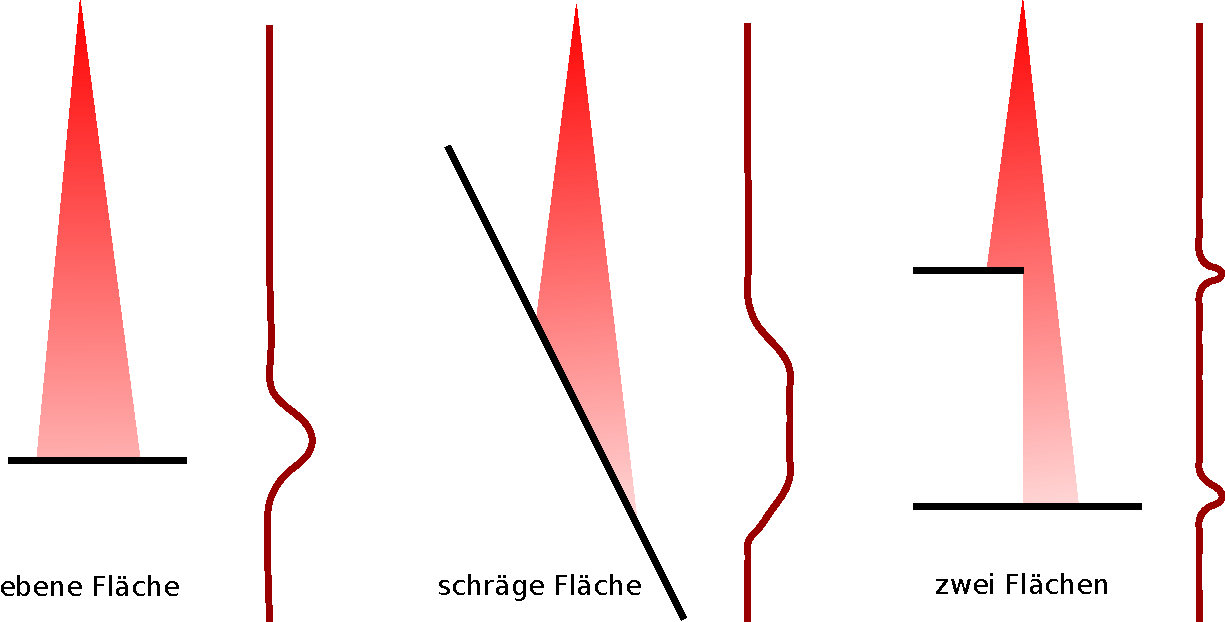
\includegraphics[width=0.7\textwidth]{./img/echo.pdf}
 % vlp16.jpg: 0x0 pixel, 300dpi, 0.00x0.00 cm, bb=
 \caption{Reflektiertes Signal nach Oberfläche, nach \citet[S. 28]{beraldin}}
 \label{img:echo}
\end{figure}

Laser\-scan\-nern mit Impulsmessverfahren ermöglichen typischerweise bis zu vier einzelne Echos aufzuzeichnen. Alternativ gibt es Scanner, die das komplette Signal mit einer Abtastrate von bis zu 0,5 Nanosekunden digitalisieren. Hier ist es dann möglich, spezielle Auswertung aufgrund der Wellenform im Postprocessing durchzuführen. \citep[S. 29]{beraldin}

\section{Positionsbestimmung mittels globalen Navigationssatellitensystemen}
\label{s:GNSS}
Zur Bestimmung der Position des Fluggerätes wird ein Empfänger für globale Navigationssatellitensysteme (global navigation satellite system, GNSS) verwendet. Ein solcher Empfänger kann durch die Laufzeitbestimmung des Signales von verschiedenen Satelliten zum Beispiel des US-amerikanischen Navstar GPS seine aktuelle Position bestimmen. Hierzu ist eine freie Sicht zum Himmel notwendig. Je nach Auswertung und Weiterverarbeitung des Signales sind Genauigkeiten zwischen 10 Metern ohne zusätzliche Daten und wenigen Millimetern bei statischen Dauermessungen und dem Einsatz von Daten von Referenzstationen im Postprocessing möglich. Es befinden sich pro System etwa 30 Satelliten in einer bekannten Umlaufbahn. Durch an Bord befindliche Atomuhren können die Satelliten hochgenaue Zeitstempel und sich wiederholende Codemuster aussenden. Im Fall von Navstar GPS erfolgt die Aussendung aktuell auf drei verschiedenen Frequenzen L1, L2 und L5. Für die öffentliche Nutzung ist nur L1 freigegeben. L2 und L5 sind der militärischen Nutzung vorbehalten. Durch reine Auswertung des ausgesendeten L1-Codes können Genauigkeiten bis 5 Meter erreicht werden. Für geodätische Anwendungsfälle wird zusätzlich die Phasenmessung benutzt. Hierbei wird nicht nur das dem Funksignal aufmodelierte Codemuster ausgewertet, sondern auch die Phase des Signals. Hierdurch ist es auch möglich, dass verschlüsselte L2-Signal mitzunutzen. Durch die Nutzung von Referenzstationsnetzen wie SAPOS können Genauigkeiten von 1-2cm in Echtzeit und von unter Zentimetergenauigkeit im Postprocessing erreicht werden \citep[S. 375]{Witte2006}.

\section{Inertiale Messeinheit}
\label{s:IMU}
Bei der inertialen Messeinheit (inertial measurement unit, IMU) handelt es sich um einen Sensor, der die Neigung sowie Drehbewegungen der Sensoreinheit misst. Sie wird benötigt, um beim Airborne Laserscanning die genaue Ausrichtung des Laser\-scan\-ners zu bestimmen. Daher muss diese auch verwindungssteif mit dem Laser\-scan\-ner verbunden sein. In Kombination mit den Positionsdaten des GNSS-Modules ermöglicht sie die Rekonstruktion der Flugbewegungen (Trajektorie). Ein weiterer Vorteil der inertialen Messeinheit ist ihre Messfrequenz: Im Gegensatz zum GNSS, dass im Normalfall nur eine Messung pro Sekunde durchführt, kann die IMU bis zu 500 Messungen pro Sekunde ausführen. Sie stützt daher nicht nur die GNSS-Messung sondern hilft auch, die Trajektorie zu interpolieren und somit auch für den Bereich zwischen den GNSS-Messungen genaue Positionen zu bestimmen. \citep[S. 23ff]{beraldin}

Die Messung erfolgt mit mehreren Einzelsensoren: Für die Messung der Beschleunigung in drei Dimensionen sind drei jeweils rechtwinklig zueinander stehende Beschleunigungsmesser verbaut. In der klassischen Bauform ist hierfür jeweils eine Probemasse zwischen zwei Federn gelagert. Durch eine auf die Probemasse wirkende Beschleunigung wird diese zwischen den Federn ausgelenkt. Die Messung der Drehrate erfolgt mittels drei einzelnen Kreiselinstrumenten (Gyroskop) in drei Achsen. Sie basieren auf Kreiseln, welche drehbar gelagert sind. Sie streben dazu, die Ausrichtung ihrer Drehachsen im Raum beizubehalten. Durch Messung der Kräfte kann die Drehrate berechnet werden. Einige inertiale Messeinheiten enthalten auch ein dreidimensionales Magnetometer, mit dem sich die magnetische Nordrichtung dreidimensional feststellen lässt.

Die Genauigkeit von inertialen Messeinheiten wird in ihre Messgenauigkeit und in ihre zeitliche Abweichung unterteilt. Die zeitliche Stabilität ist vorallem bei der Inertialnavigation, die ausschließlich auf deren Messungen basiert, wichtig.

\begin{figure}
 \centering
 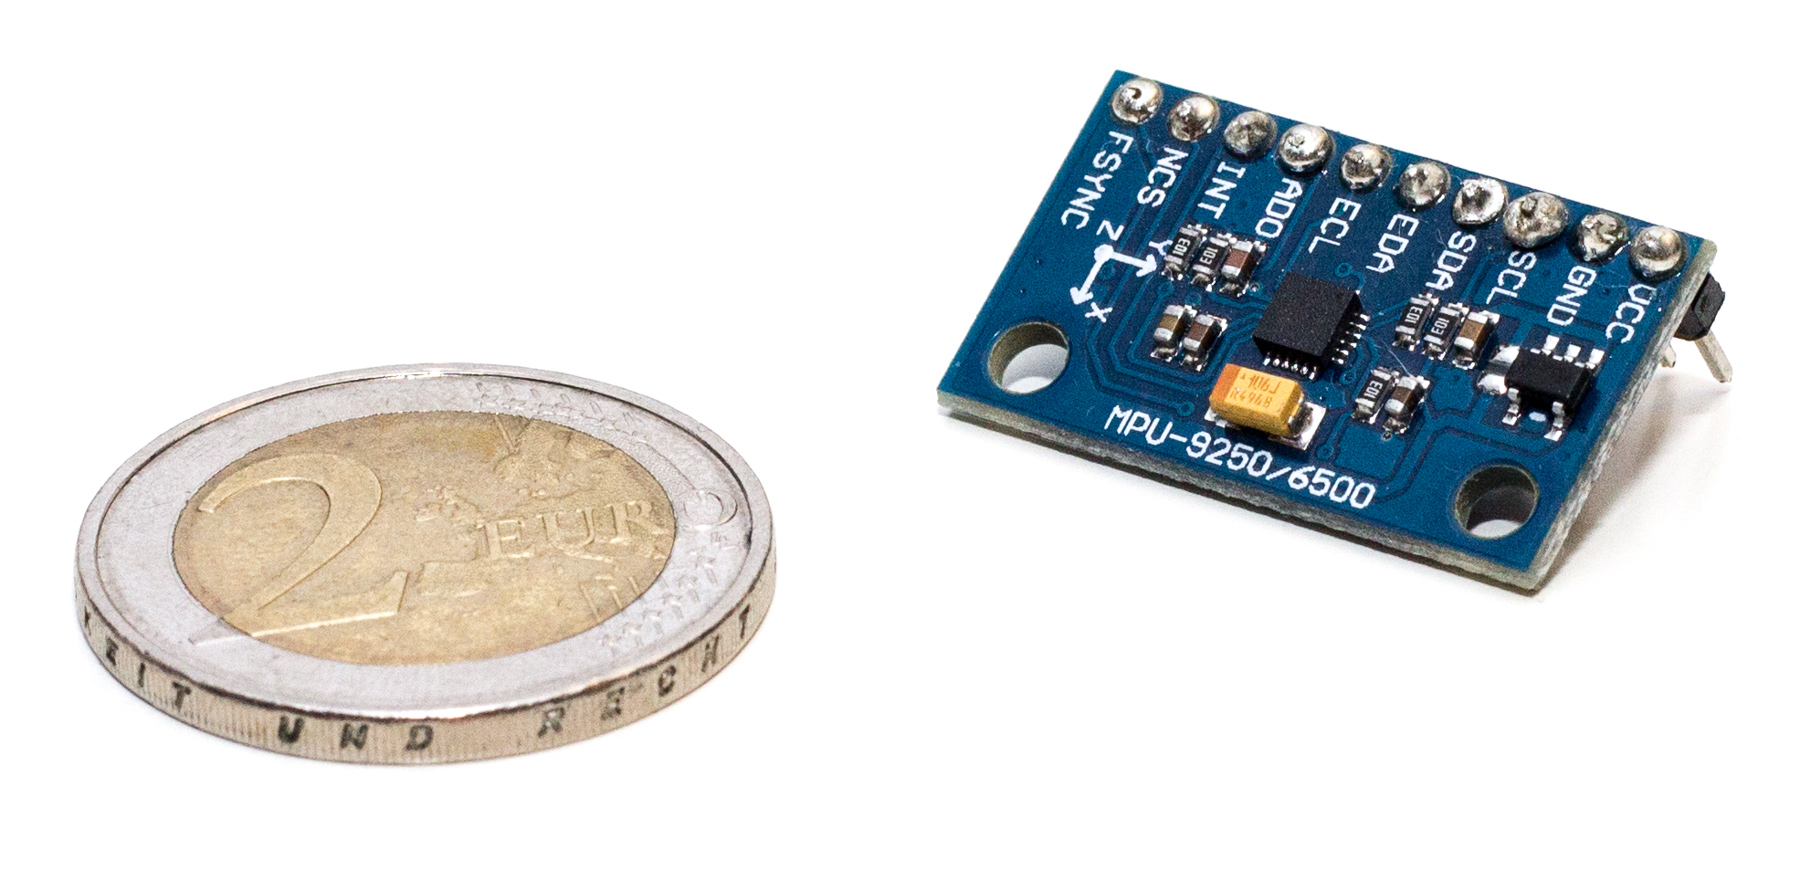
\includegraphics[width=0.7\textwidth]{./img/mems.jpg}
 % vlp16.jpg: 0x0 pixel, 300dpi, 0.00x0.00 cm, bb=
 \caption{MPU-9250 - Low-Cost-MEMS-IMU-Modul wie es in vielen Consumer-Geräten und Multikoptern verwendet wird (schwarzes Bauteil mittig auf der Platine, eigene Aufnahme)}
 \label{img:mems}
\end{figure}

Hauptsächlich unterschieden werden die inertialen Messeinheiten in klassische, mechanische Systeme, wie sie bereits hier beschrieben wurden, und mikroelektromechanische Systeme, sogenannte MEMS (microelectromechanical systems). Bei den zweitgenannten handelt es sich um stark miniaturisierte Bauteile (beispielsweise \autoref{img:mems}) , welche zum Beispiel in aktuellen Smartphones eingesetzt werden. Sie werden für Zwecke eingesetzt, in denen keine hohen Genauigkeitsanforerungen gestellt werden und der Preis gering gehalten werden soll. Auch zur Stabilisierung der Fluglage von Multikoptern oder Gimbals werden diese Sensoren eingesetzt. Für geodätische Anwendungsfälle werden jedoch meist noch mechanische Systeme genutzt, da deren Genauigkeit und ihre zeitliche Abweichung geringer sind. Höherpreisige MEMS-Sensoren erreichen bereits gute Genauigkeiten.

\todo{Quelle}

\section{Kombination des Messsysteme}
Um die drei eigenständigen Messsysteme kombiniert nutzen zu können, muss die relative Position der Systeme genau bekannt sein und darf sich während des Fluges nicht verändern. Beim klassischen Airborne Laserscanning vom Helikopter werden hierfür zum Beispiel eigenständige Module entwickelt, die alle benötigten Systeme verdrehsicher enthalten und an den Kufen des Helikopters montiert werden können \citep[S. 23f]{beraldin}

Außerdem müssen alle Systeme synchronisiert werden, damit die Daten später miteinander verarbeitet werden können. Hierfür wird üblicherweise das Sekundensignal des Navigationssatellitensystems (pulse per second, PPS) genutzt. Das GNSS-System sendet dazu zu jeder vollen Sekunde der GNSS-Zeit ein Impuls aus, mit welchen sich die anderen Sensorsysteme synchronisieren können. 

\section{Bisherige Systeme zur dreidimensionalen Erfassung mittels Multikoptern}
Die meisten aktuellen Verfahren zur Erzeugung von 3D-Modellen unter Nutzung von kompakten Multikoptern mit einer Tragkraft von bis zu 5kg, basieren auf photogrammetrischen Verfahren. Sie erzeugen Bilder, meist unter direkter Georeferenzierung, welche im Postprocessing zu Bildverbänden verknüpft werden. Mittels Bilderkennung werden hieraus 3D-Punktwolken berechnet. Nachteil dieses Verfahrens ist es, dass ausreichende Beleuchtung vorhanden sein muss. Es kann somit nur tagsüber geflogen werden, aber auch starke Schatten können das Ergebnis verschlechtern. Für die automatische Erstellung von Punktwolken muss außerdem das Gelände ausreichende Strukturen aufweisen, damit automatische Verknüpfungen der Pixel erfolgen können.

Laserscanning als aktiver Sensor hat hier den Vorteil, dass keine zusätzliche Beleuchtung benötigt wird -- der Sensor bringt sein Licht selber mit. Problematisch ist hierbei jedoch die Größe der Systeme. Aus diesem Grund wurden bisher hauptsächlich Systeme mit großen UAVs erprobt und verwendet \citep[S. 19]{uav}. Durch die immer weiter fortschreitende Miniaturisierung und die Weiterentwicklung von Laser\-scan\-nern zum Beispiel für die Entwicklung von autonomen Fahrzeugen werden die Scanner auch inzwischen kleiner und leistungsfähiger.

\todo{Quelle, füllen}

\chapter{Technische Realisierung}
\label{c:realisierung}


Im Folgenden wird zunächst auf die verwendeten Geräte und ihre technischen Eigenschaften eingegangen, bevor danach auf die technischen Verbindungen eingegangen wird.

\section {Verwendete Gerätschaften}

\subsection{Velodyne VLP-16}
\label{sss:vlp16}
Um Gewicht zu sparen, wird für die Messung ein miniaturisierter Laser\-scan\-ner eingesetzt. Einer dieser Kompakt-Laser\-scan\-ner ist der Velodyne Puck VLP-16 (siehe \autoref{img:vlp16}). Er hat einen Durchmesser von etwa 10 cm und eine Höhe von 7 cm bei einem Gewicht von etwa 830 g ohne Kabel und Schnittstellenbox. Es handelt sich beim VLP-16 wahrscheinlich um einen Faserscanner (siehe \autoref{p:faserscanner}) mit 16 Messstrahlen, der sich zusätzlich um seine Hochachse dreht. Genaue Angaben macht der Hersteller hierzu keine. Seine Messgenauigkeit beträgt laut Datenblatt \(3~cm\). Gemessen wird im Impulsmessverfahren (siehe \autoref{p:tof}) mit einem Infrarotlaser mit einer Wellenlänge von 903nm. \citep{vlpSheet}

Der Scanner sendet die Messstrahlen mit einem Zeitabstand von \(2,3\mu s\) hintereinander aus, gefolgt von einer Nachladezeit von \(18,4\mu s\), so dass jeder Messstrahl alle \(55,3~\mu s\) ausgesendet werden kann \citep[S. 16]{vlpManual}. Es ergibt sich somit eine durchschnittliche Messfrequenz von \(289.357~Hz\) (siehe \autoref{equ:XproS}). Während der Messungen dreht sich der Laser\-scan\-ner je nach Einstellung über das Webinterface des Scanners mit 5 bis 20 Umdrehungen pro Sekunde \citep{vlpSheet}. Pro ausgesendeten Strahl können jeweils die erste und die stärkste Reflexion zurück gegeben werden, so dass über eine halbe Million Punkte pro Sekunde gemessen werden können (siehe \autoref{equ:XproS}). Die Daten werden anschließend über den Netzwerkanschluss gestreamt (siehe auch \autoref{ss:Datenlieferung}). Außerdem verfügt der Scanner über einen Anschluss für ein GNSS-Modul des Types Garmin GPS 18x LVC. Auch andere GNSS-Module sind nutzbar, so dass im Weiteren der Versuch unternommen wurde, hier das GNSS-Modul der inertialen Messeinheit (siehe \autoref{s:iMar}) oder eines uBlox-GNSS-Modules zu nutzen (siehe \autoref{s:GNSSAnschluss}). Durch die Nutzung eines GNSS-Modules am Scanner ist es möglich, die Daten mit einem hochgenauen Zeitstempel zu versehen und die Messungen des Scanners so in der Nachbearbeitung mit den Daten aus der inertialen Messeinheit zu verknüpfen.

\begin{equation}
 \label{equ:XproS}
 \begin{aligned}
  f &= \frac{1s}{55,295\mu s} \cdot 16~\frac{Messstrahlen}{Messung} = 289.357~\frac{Messung}{Sekunde} \\
  n &= 289.357~\frac{Messung}{Sekunde} \cdot 2~\frac{Messwerte}{Messtrahl} = 578.714~\frac{Messwerte}{Sekunde}
 \end{aligned}
\end{equation}

\begin{figure}
 \centering
 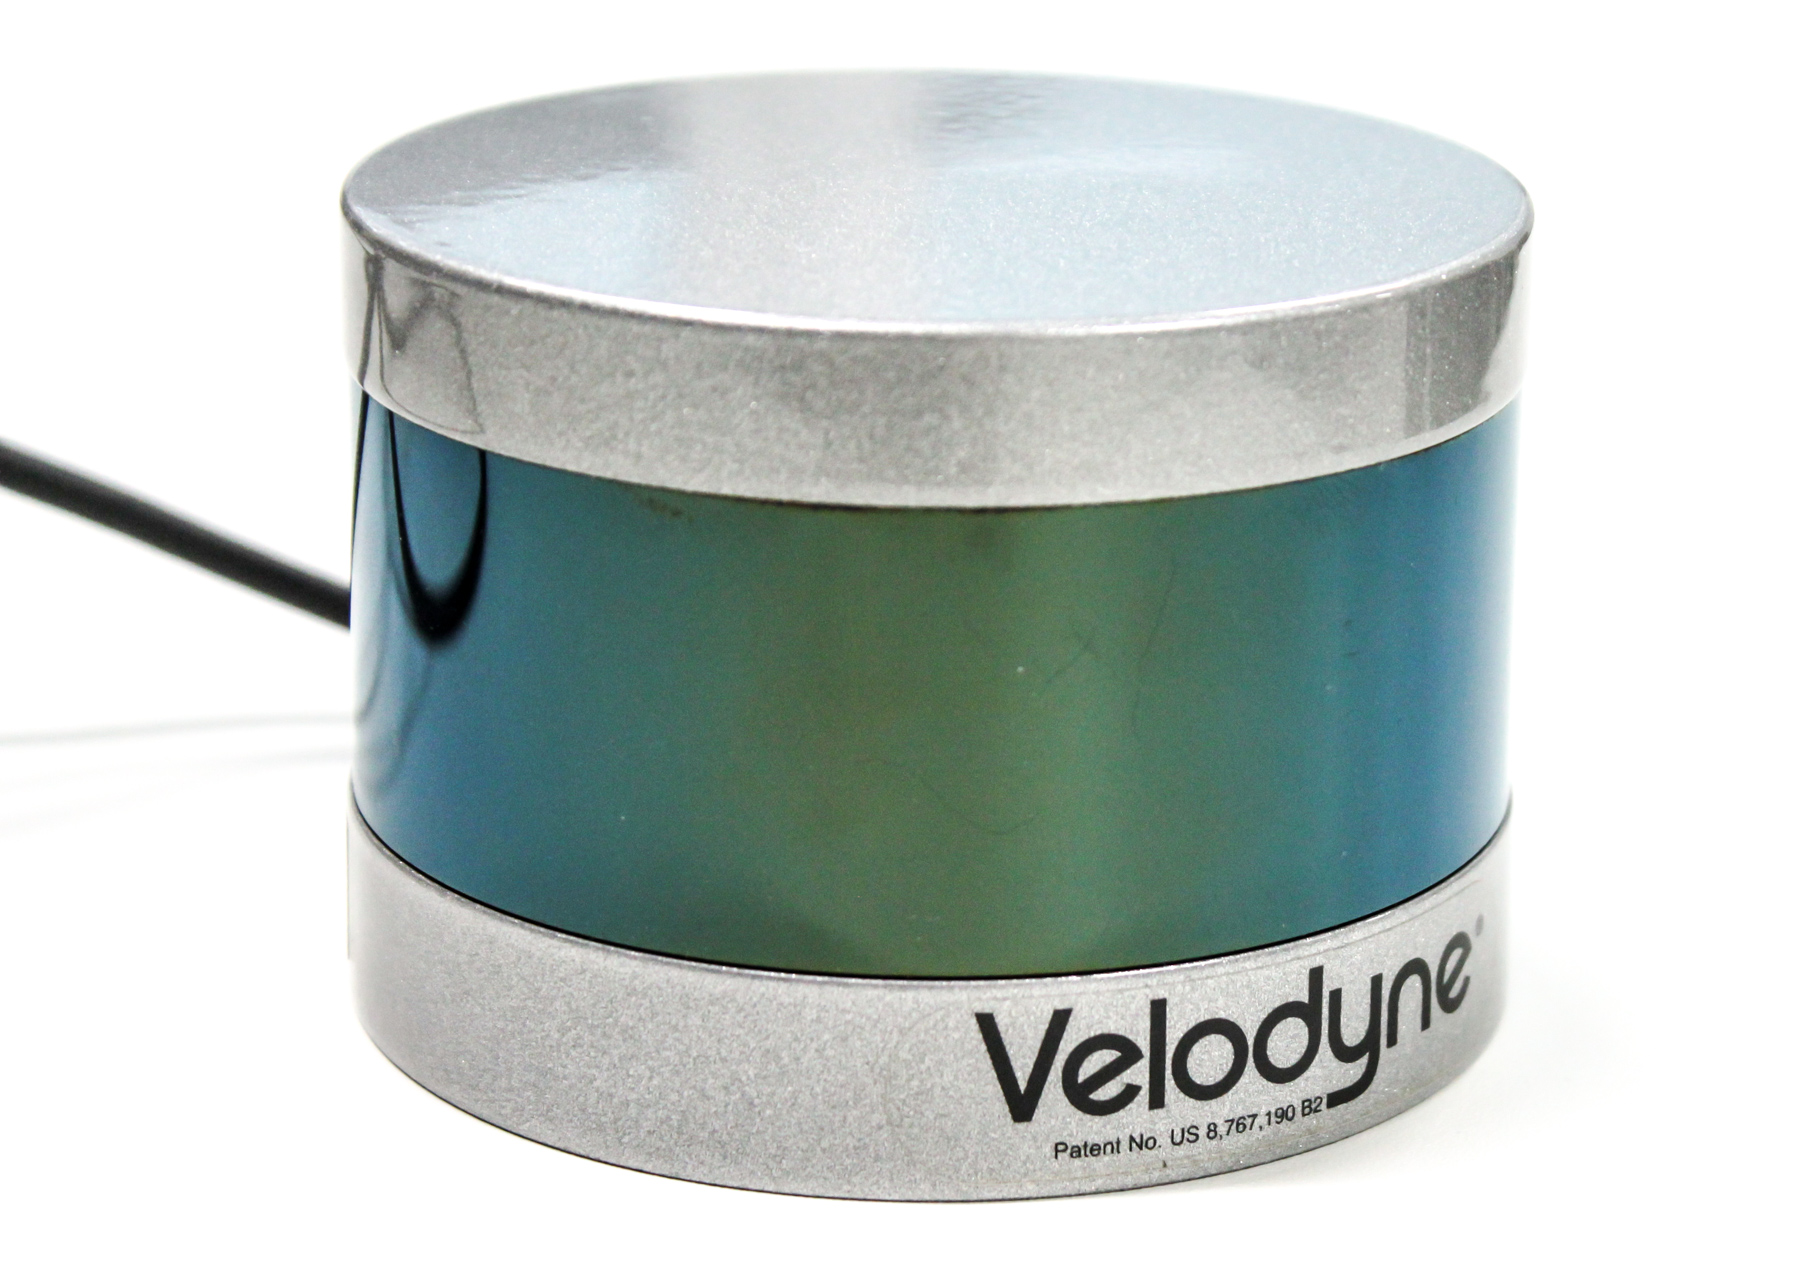
\includegraphics[width=0.7\textwidth]{./img/vlp16.jpg}
 % vlp16.jpg: 0x0 pixel, 300dpi, 0.00x0.00 cm, bb=
 \caption{Laser\-scan\-ner Velodyne VLP-16 (eigene Aufnahme)}
 \label{img:vlp16}
\end{figure}

\subsection{Inertiale Messeinheit und GNSS-Empfänger iMAR iNAT-M200-FLAT}
\label{s:iMar}
Als inertiale Messeinheit wird das auf \autoref{img:imu} zu sehende Sensorsystem des Typs iMAR iNAT-M200-FLAT verwendet. Hierbei handelt es sich um ein hochgenaues MEMS-System. Durch die Verwendung von mikroelektromechanischen Bauteilen wiegt der Sensor inklusive Gehäuse nur 550 Gramm. Er kann bis zu 500 Messungen pro Sekunde durchführen. Die Abweichung der Richtungsmessungen pro Stunde liegt unter 0,5 Grad. \citep{imar}
\todo{Messgenauigkeit}

\begin{figure}
 \centering
 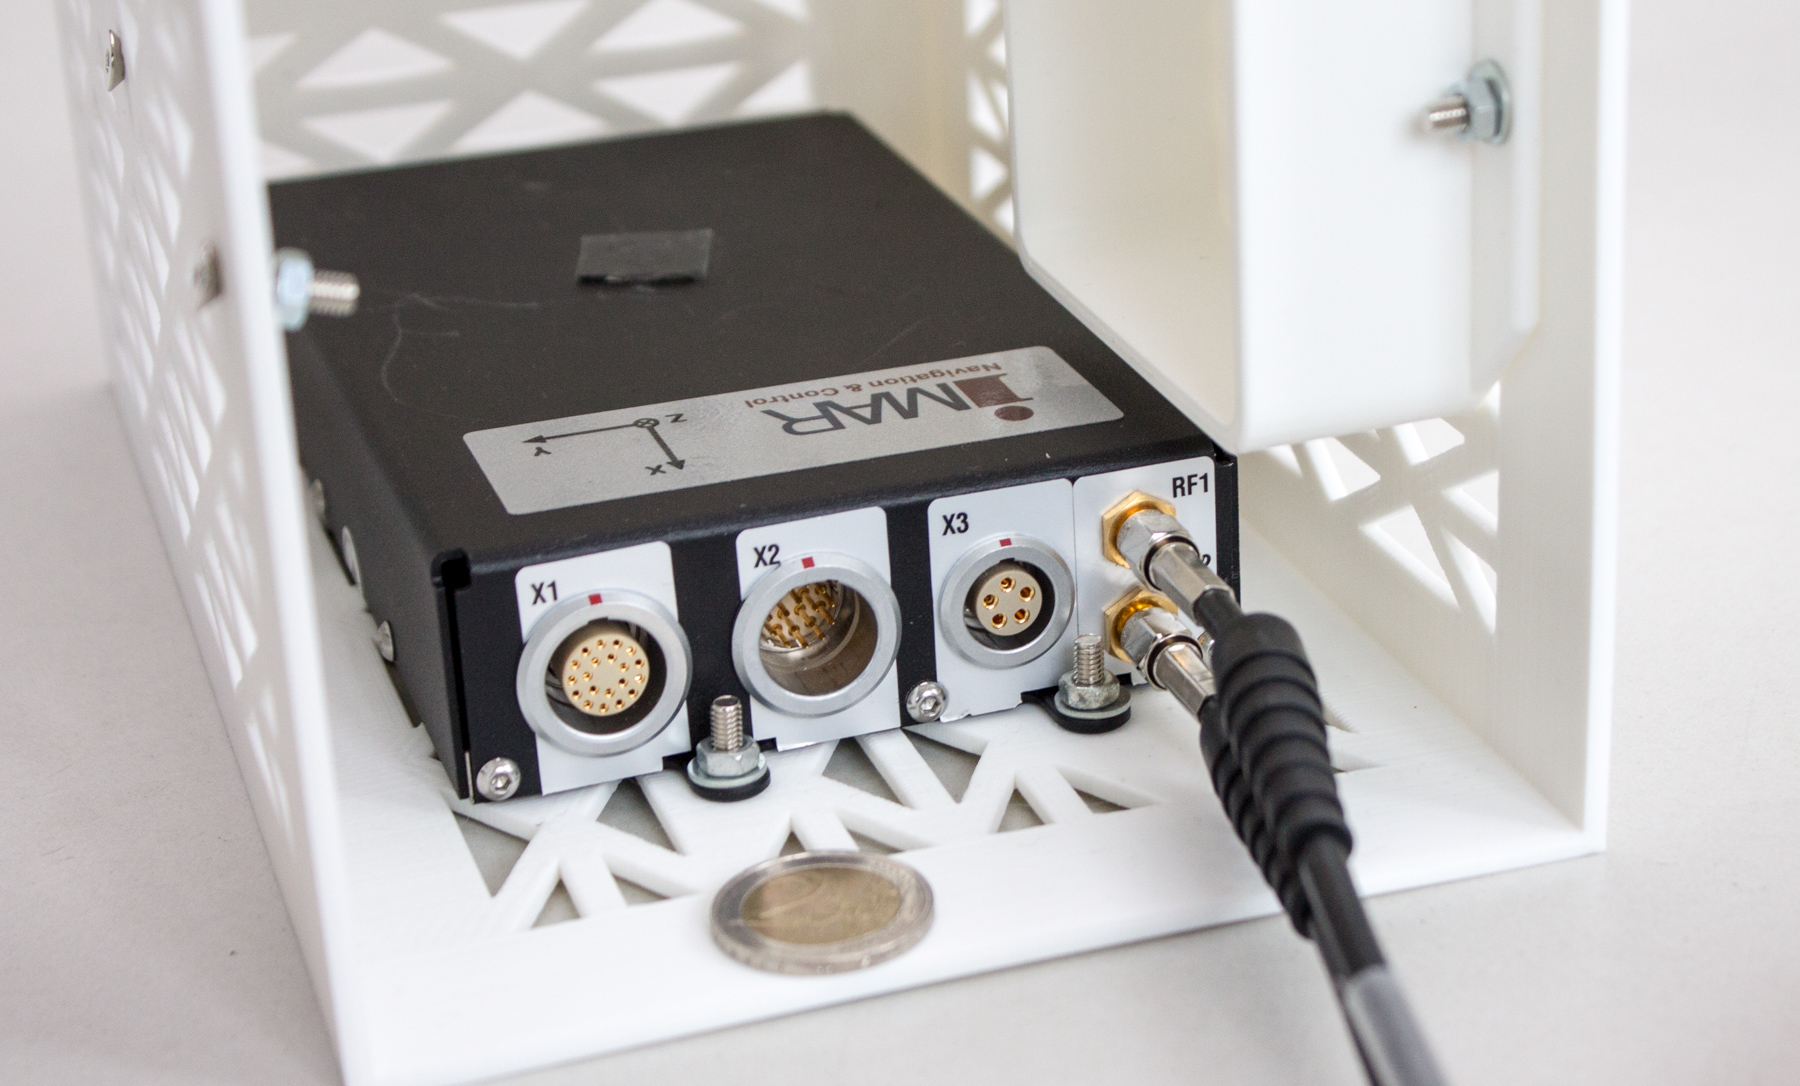
\includegraphics[width=0.7\textwidth]{./img/imu.jpg}
 % vlp16.jpg: 0x0 pixel, 300dpi, 0.00x0.00 cm, bb=
 \caption{iMAR iNAT-M200-Flat im Prototypen des modularen Gehäuses, Leitungen führen zu den GNSS-Antennen (eigene Aufnahme)}
 \label{img:imu}
\end{figure}

Außerdem verfügt die verwendete Einheit über zwei differentielle Satellitennavigationsempfänger (GNSS-Module, siehe \autoref{img:gnss}). Durch Nutzung einer zusätzlichen GNSS-Basisstation oder auch einem entsprechenden Korrekturdienst können diese eine Positionsgenauigkeit von etwa 2 Zentimeter in Echtzeit erreichen \citep{imar}. Durch Postprocessing lässt sich diese sogar noch steigern. \citet{wilken} \todo{alternativ: Matthias Wilkens} Durch die Verwendung von zwei Empfängern, die an jeweils einem Ausleger befestigt sind (siehe Bild \autoref{img:gnss}), kann auch die Orientierung des Scanners bestimmt werden. Hierdurch wird die ungenaue Messung des magnetischen Nordpols überflüssig. Außerdem kann die Positionssicherheit durch Mittlung der beiden Positionen erhöht werden.

\begin{figure}
 \centering
 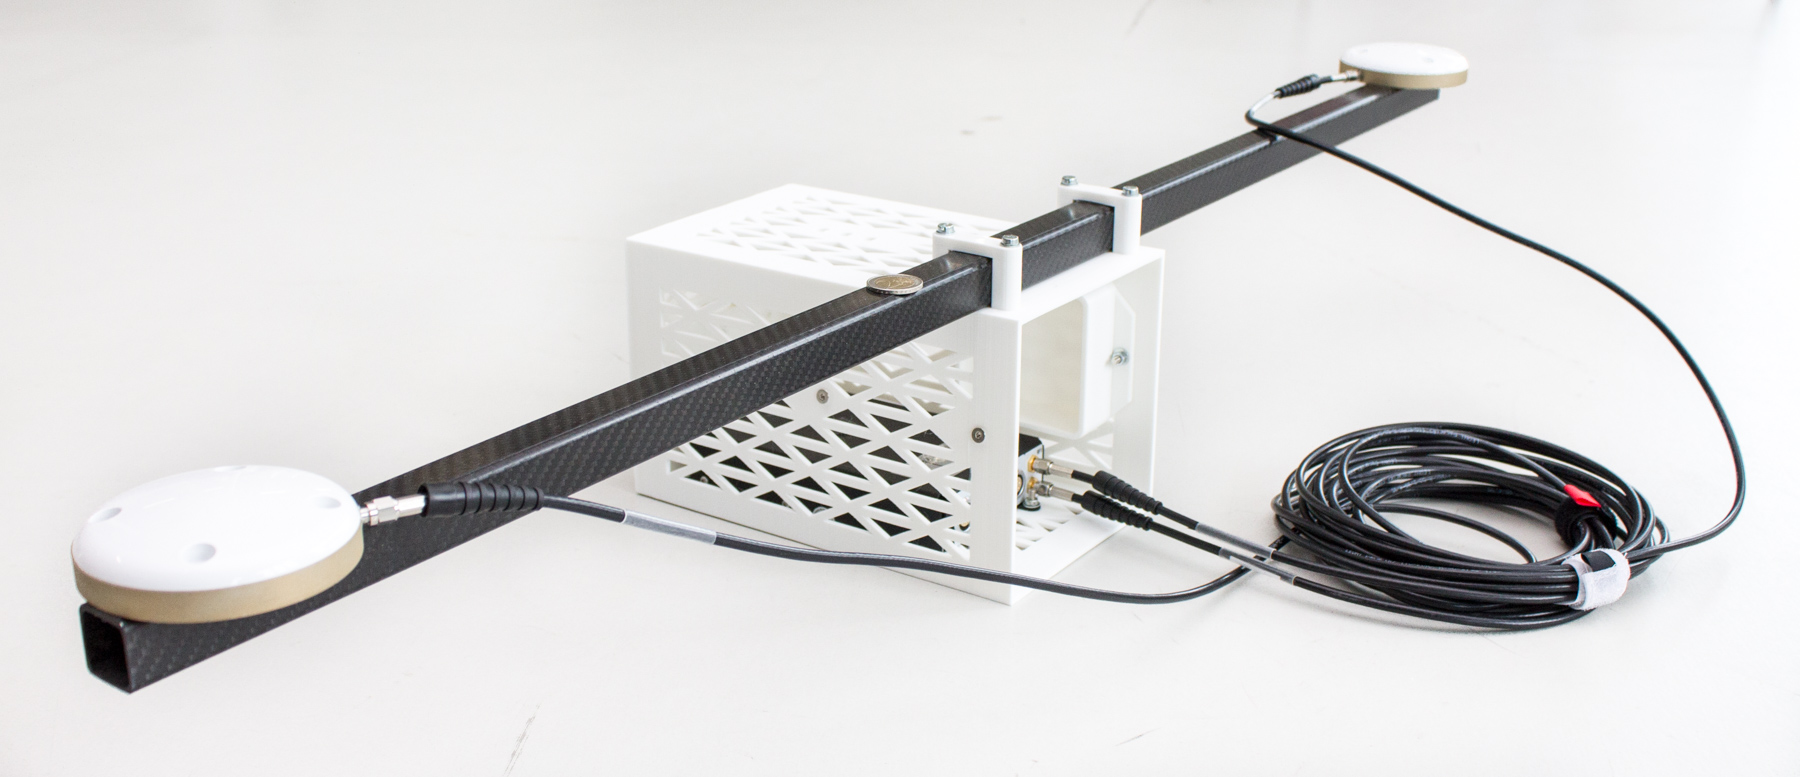
\includegraphics[width=0.8\textwidth]{./img/gnss.jpg}
 % vlp16.jpg: 0x0 pixel, 300dpi, 0.00x0.00 cm, bb=
 \caption{GNSS-Antenennen des (links und rechts) iMAR iNAT-M200-Flat an Prototypen des modularen Gehäuses (eigene Aufnahme)}
 \label{img:gnss}
\end{figure}

Im Postprocessing kann aus den Daten der inertialen Messeinheit zusammen mit denen der GNSS-Module und GNSS-Korrekturdaten eine genaue Flugbahn des Multikopters berechnet werden. Die Daten der inertialen Messeinheit werden hierbei regelmäßig durch die Daten der GNSS-Module gestützt.

\subsection{Raspberry Pi 3 Typ B}
\label{ss:Raspberry}
Es wurde sich entschieden, die Datenverarbeitung mit einem Raspberry Pi 3 (siehe \autoref{img:rpi3}) durchzuführen. Es handelt sich hierbei um einen von der Raspberry Pi Foundation entwickelten Einplatinencomputer. Die Stiftung gründete sich 2006, um einen erschwinglichen Computer zu entwickeln, an den Schüler direkt Hardware- und Elektronikprojekte entwickeln können. Die erste Version des Raspberry Pi kam im Februar 2012 auf den Markt. Er verfügte über 256 MB Arbeitsspeicher und einen 700 MHz Ein-Kernprozessor. Das verwendete dritte Modell verfügt über einen Vier-Kern-Prozessor mit 1,2 Ghz und 1 GB Arbeitsspeicher. Bisher wurden alle Versionen zusammen über 11 Millionen mal verkauft. \citep{heise5Rasp}

Alle Modelle der Raspberry Pi Serie basieren auf Ein-Chip-Systemen des Halbleiterherstellers Broadcom. In diesem Chip sind die wichtigsten Bauteile des Systems integriert wie ein ARM-Prozessor, eine Grafikeinheit sowie verschiedene andere Komponenten. Die so gering gehaltene Anzahl an einzelnen Bauelementen beim Raspberry Pi ermöglichen den geringen Preis - ein Ziel der Raspberry Pi Foundation.

Der Vorteil des Raspberry Pi zur Datenverarbeitung sind vor allem seine verschiedensten Schnittstellen zur Daten Ein- und Ausgabe \citep{raspSheet}:
\begin{itemize}
 \item 4 USB 2.0 Host-Anschlüsse
 \item Netzwerkschnittstelle (RJ45)
 \item Bluetooth- und WLAN
 \item 27 GPIO-Ports, nutzbar als \citep{ekRaspPin}
 \begin{itemize} 
  \item Digitale Pins
  \item Serielle Schnittstelle
  \item I2C-Schnittstelle
  \item SPI-Schnittstelle
 \end{itemize}
 \item Stromversorgung 3,3V und 5V
 \item MicroUSB-Anschluss zur eigenen Stromversorgung (5V)
 \item MicroSD-Steckplatz 
 \item verschiedene Video- und Audioausgänge
 \end{itemize}

Außerdem vorteilhaft für die Nutzung am Multikopter ist seine geringe Größe und sein relativ geringer Stromverbrauch von maximal 12,5 Watt \citep{raspSheet}. Im Betrieb ohne Peripherie wird dieser Stromverbrauch bei weitem nicht erreicht, hier liegt der Stromverbrauch bei etwa \todo{Messung}.

\begin{figure}
 \centering
 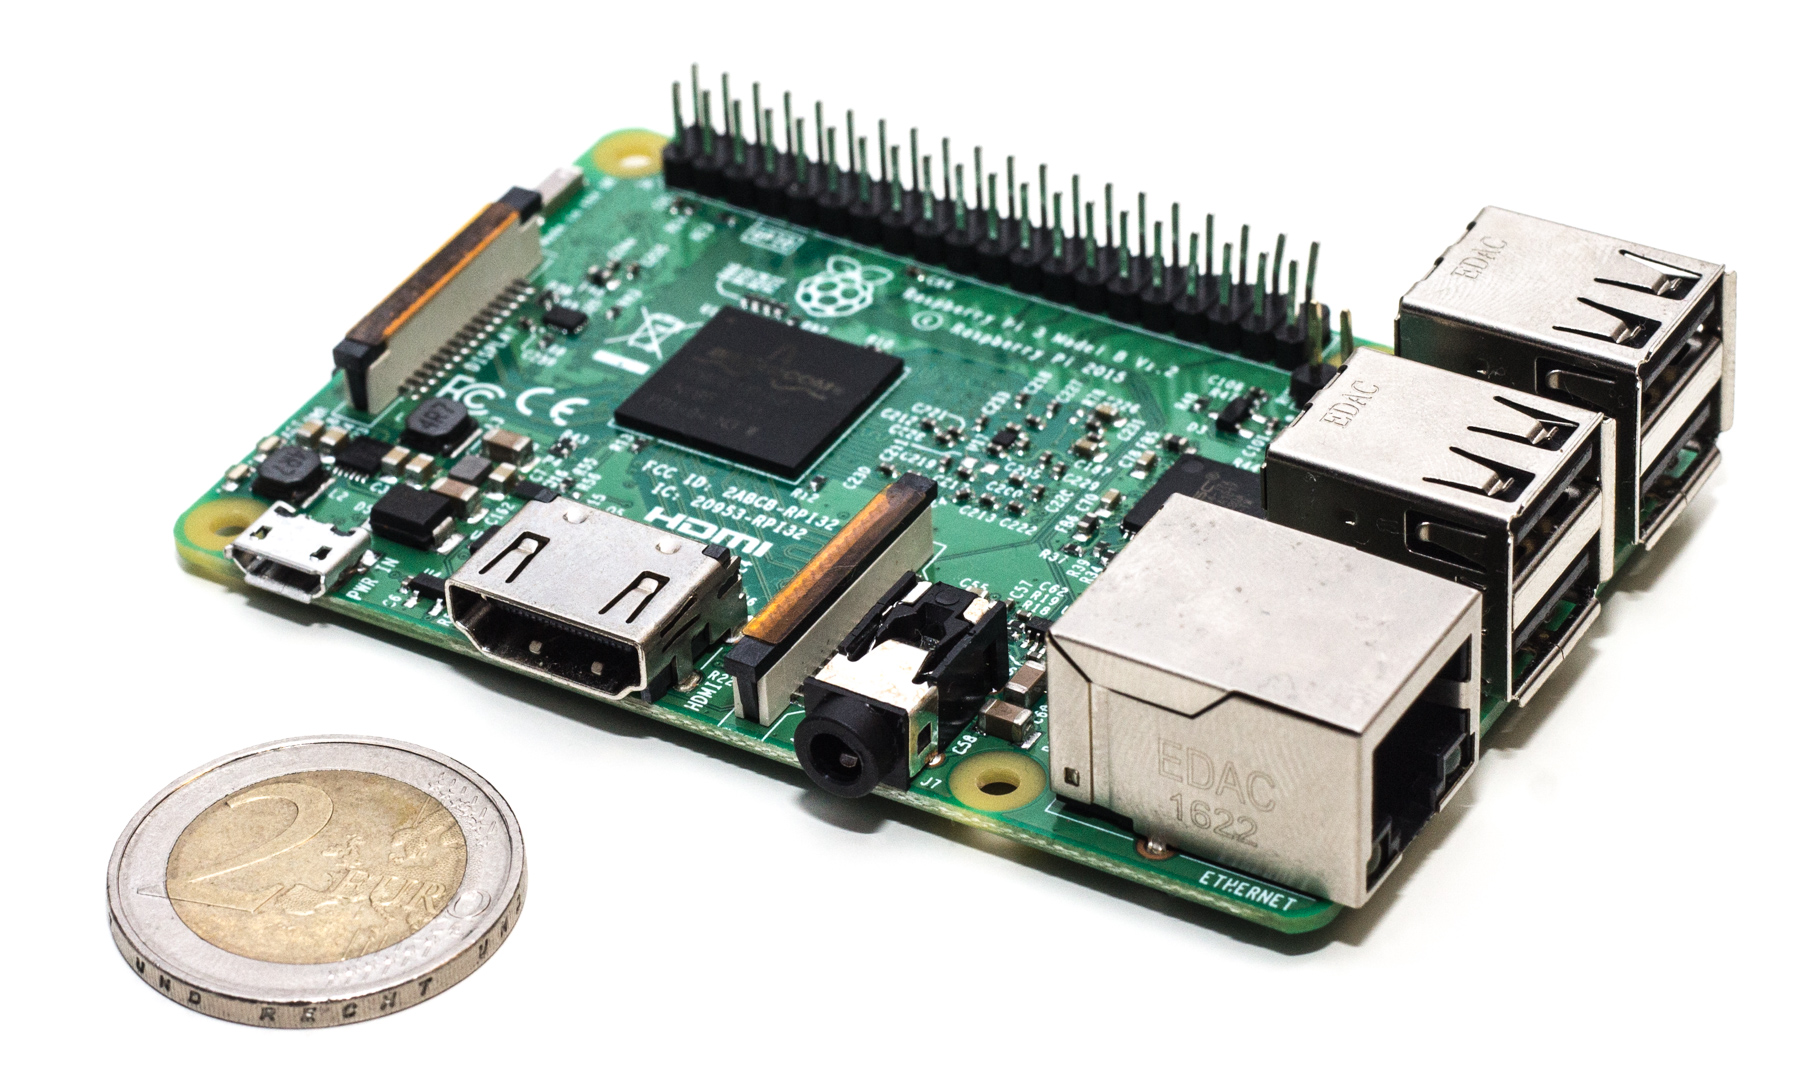
\includegraphics[width=0.7\textwidth]{./img/rpi3.jpg}
 % vlp16.jpg: 0x0 pixel, 300dpi, 0.00x0.00 cm, bb=
 \caption{Raspberry Pi 3 (eigene Aufnahme)}
 \label{img:rpi3}
\end{figure}

\subsection{Multikopter Copterproject CineStar 6HL}
Bei einem Multikopter handelt es sich um ein Fluggerät mit drei oder mehr Rotoren. Es gibt entsprechend der Rotoranzahl verschiedene Modelle wie zum Beispiel den weit verbreiteten Quadrokopter oder den Hexakopter, welcher in dieser Arbeit betrachtet wird. Multikopter wurden ursprünglich für Militär- und Polizeizwecke eingesetzt, inzwischen sind sie aber auch vermehrt in kleineren Ausführungen im Privatbesitz für Videoaufnahmen zu finden \citep{Quadro}. Angetrieben werden die handelsüblichen Modelle, welche eine Flugdauer von bis zu 30 Minuten und eine Tragkraft von bis zu fünf Kilogramm versprechen, mit Lithium-Polymer-Akkumulatoren (LiPo-Akkus). Die Anzahl und die maximale Umdrehung der Rotoren bestimmt die Schubkraft und somit auch die Tragkraft des Multikopters. Im Normalfall ist die Anzahl der Rotoren durch zwei teilbar, damit sich das auf das Traggestell wirkende Drehmoment aufhebt. Dies ist der große Vorteil gegenüber einem Hubschrauber, bei welchem mit einem Heckrotor dem Drehmoment um die Hochachse entgegengewirkt werden muss. Die einzelnen Motoren und Propeller werden kreuzweise angeordnet, so dass eine Drehzahländerung eines Propellerpaares zur Steuerung ausreicht. Vorteil eines Multikopters im Gegensatz zu einem Modellflugzeug ist es außerdem, dass er senkrecht starten kann und auch zum Beispiel für die Aufnahme von Bildern auf der Stelle stehen bleiben kann. Nachteil ist der höhere Energieverbrauch, so dass Flugzeuge bei gleicher Akkukapazität deutlich länger in der Luft bleiben können. \citep{Bachfeld}

\begin{figure}
 \centering
 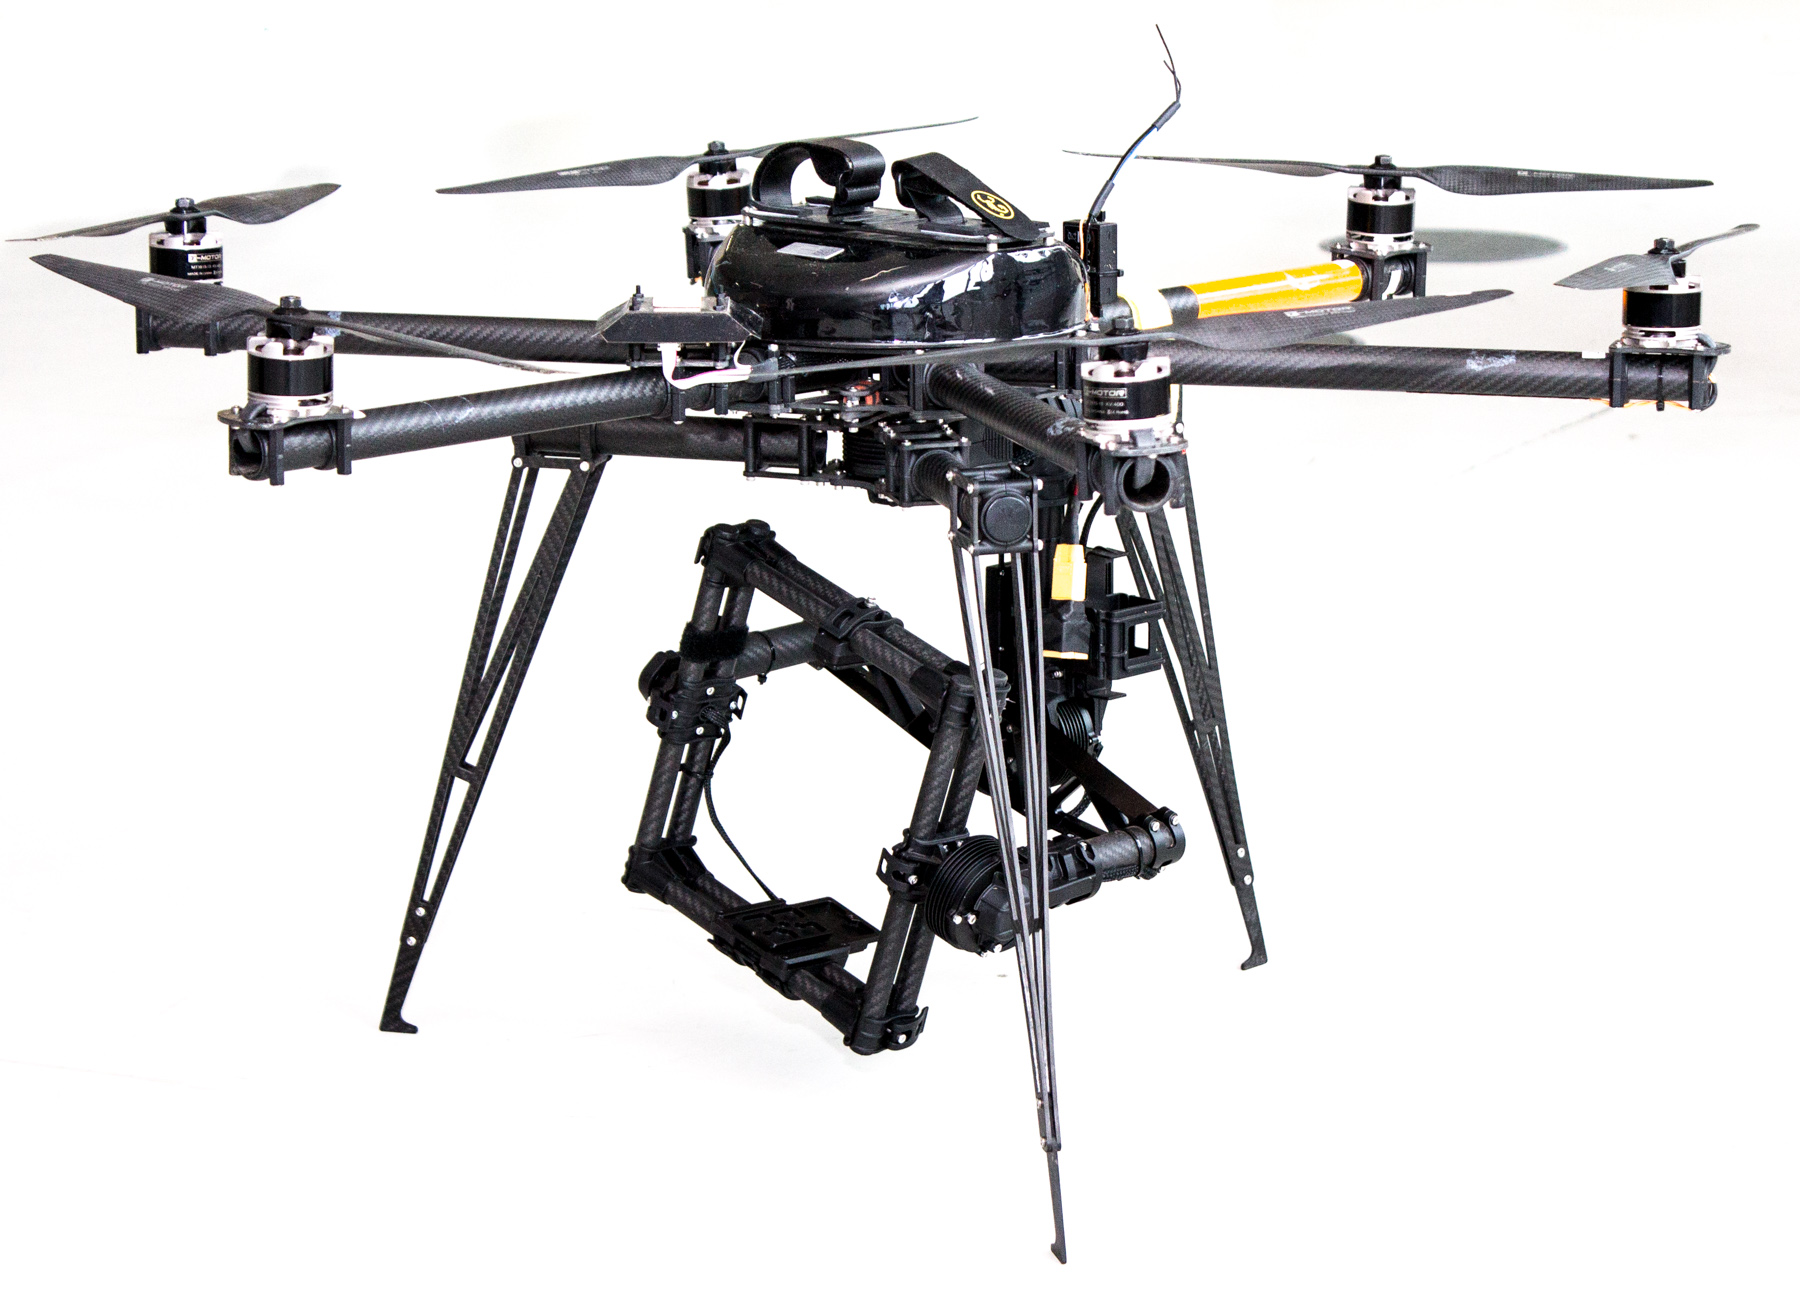
\includegraphics[width=0.7\textwidth]{./img/uav.jpg}
 % vlp16.jpg: 0x0 pixel, 300dpi, 0.00x0.00 cm, bb=
 \caption{Multikopter Copterproject CineStar 6HL mit Gimbal Freefly MöVI M5 (eigene Aufnahme)}
 \label{img:uav}
\end{figure}

In dieser Arbeit soll der Multikopter den Laser\-scan\-ner, die IMU, das Gimbal, die Stromversorgung, Datenverarbeitung und -speicherung im Betrieb tragen können. Bei der Systementwicklung des Multikopters muss daher darauf geachtet werden, dass das Gewicht möglichst gering bleibt und dennoch müssen die angehängten Messeinrichtungen auch für härtere Landungen ausgelegt sein. Der verwendete Hexakopter (siehe \autoref{img:uav}) hat eine Tragkraft von maximal 5 Kilogramm und eine Flugdauer von bis zu 20 Minuten \citep{Schulz}.

\subsection{Gimbal Freefly MöVI M5}
Um die Messgeräte während des Fluges des Multikopter zu stabilisieren und zu verhindern, dass sich jede Neigung der Flugsteuerung an den Laser\-scan\-ner überträgt, wird ein sogenanntes Gimbal verwendet. Durch einen Regelkreis aus Motoren und einer inertialen Messeinheit (siehe auch \autoref{s:IMU}), werden Neigungen und Drehungen in Echtzeit ausgeglichen. Außerdem ist es durch viele Gimbals möglich, die Messtechnik unabhängig vom Multikopter auszurichten - dies ist zum Beispiel bei der Luftbildaufnahme wichtig.

Für das Projekt wird ein Gimbal des Herstellers Freefly verwendet. Sie wird eigentlich zur Stabilisierung von Aufnahmen mit digitalen Spiegelreflexkameras entwickelt. Sie hat eine Tragkraft von 2,3 Kilogramm. Außer den erwähnten Beschleunigungsmesser verwendet diese auch GNSS um das driften der integrierten IMU zu vermindern. \citep{movim5}


\section{Auswahl des Datenverarbeitungssystems}

Ein Teil der Datenverarbeitung und die Speicherung soll direkt auf dem Sensorsystem durchgeführt werden. Da bei dem Betrieb des Multikopters jede weitere Masse die Laufzeit verkürzt, muss hierbei auf das Gewicht geachtet werden. Somit kommen für die Verarbeitung nur Ein-Chip-Computersysteme wie der Raspberry-Pi oder Mikrokontroller-Boards wie die der Arduino-Serie in Frage. 

Vorteile eines Arduinos wären vorallem der geringere Stromverbrauch und die Echt-Zeitfähigkeit. Jedoch ist die Steuerung der Datenaufnahme über die Netzwerkschnittstelle und die Speicherung deutlich komplizierter und die Hardware nicht so leistungsfähig. Bei der Alternative, dem Raspberry-Pi übernimmt das Betriebssystem die grundlegenden Steuerungen, so dass nur noch die Daten selbst verarbeitet werden müssen. Außerdem bietet er mit der festverbauten Netzwerkschnittstelle und dem MicroSD-Karten- und der USB-Schnittstelle auch die komplette benötigte Hardware, die so nicht einzeln zusammengestellt und -gebaut werden muss.


\section{Stromversorgung}
Die Stromversorgung des Raspberry Pi an dem Multikopter soll mittels Lithium-Ionen-Zellen erfolgen. Der Raspberry Pi erfordert hierbei eine stabilisierte Spannungs- und Stromversorgung. Eine fehlerhafte Stromversorgung kann hierbei zu Systeminstabilitäten führen und so im schlimmsten Fall die Datenaufzeichnung komplett verhindern. Auf den genauen Aufbau einer solchen Versorgung wird hierbei verzichtet, sondern nur die Anforderungen an die Energiequelle erläutert.

\autoref{tab:strom} listet die verschiedenen Module und die jeweils benötigte Energieversorgung auf. Der Multikopter mit der Gimbal verfügt über eine eigene Versorgung und muss daher nicht weiter beachtet werden. Außerdem hat hier eine eigene Akkukapazität auch Vorteile - auch bei einem zu hohen Verbrauch der Sensortechnik bleibt der Multikopter durch seine eigenständige Akku-Überwachung immer noch flugfähig um sicher landen zu können.

\begin{table}
\centering
\begin{tabular}{ l | r | r | r }
  Gerät 	& Laser\-scan\-ner	& IMU		& Raspberry Pi\\
  \hline
  Spannung 	& 9 - 18 V 	& 10 - 36 V	& 5,0 V \\
  \hline
  max. Strom 	& 0,9 A		& 0,75 A	& 2,5 A \\
  \hline
  typ. Leistung	& 8 W		& 7,5 W		& 12,5 W 
\end{tabular}
\caption{Spannungs- und Strombedarf der einzelnen Module \citep{vlpSheet,imar,raspSheet}}
\label{tab:strom}
\end{table}

Für eine geplante Flugdauer von 30 Minuten wird bei einem angenommenen Wirkungsgrad von 90\% eine Akkukapazität von mindestens 16 Wh (siehe \autoref{equ:akku}) benötigt. Außerdem muss ein Teil in 12 Volt und ein Teil mit 5 Volt stabilisierter Spannung abgeben werden können. Gegebenenfalls sind hierfür auch zwei komplett unabhängige Spannungsquellen zu nutzen.

\begin{equation}
\label{equ:akku}
E = \frac{ P \cdot t}{\eta} = \frac{(8~W + 12,5~W + 7,5W) \cdot 0,5~h}{90~\%} \approx 15,6~Wh
\end{equation}

\section{Anbindung des Raspberry Pi an den Laser\-scan\-ner}
Durch seine vielseitigen Anschlussmöglichkeiten bildet der Raspberry Pi den Sternpunkt der Schnittstellen. Der Laser\-scan\-ner wird mit einem RJ45-Kabel an der Netzwerkschnittstelle angeschlossen. Die inertiale Messeinheit zeichnet die Daten selbst\-stän\-dig auf, kann aber auch mittels der als serieller Schnittstelle nutzbaren GPIO-Pins an den Raspberry Pi angeschlossen werden. Außerdem kann an diesem Port auch ein GNSS-Modul angeschlossen werden. Dieses GNSS-Modul kann im Folgenden dem Raspberry Pi zu einer genauen Uhrzeit verhelfen, die für die Verarbeitung der Daten benötigt wird. Alternativ kann auch ein an den Laser\-scan\-ner angeschlossenes GNSS-Modul sein Zeitstempel per Netzwerk an den Raspberry Pi liefern. Diese Methode soll hier verwendet werden.

\section{Verbindung des GNSS-Modules zum Laser\-scan\-ner}
\label{s:GNSSAnschluss}
Für die Versorgung des Laser\-scan\-ners mit einem GNSS-Signal zur Synchronisierung wurde ein zusätzliches GNSS-Modul vom Typ uBlox NEO6M mit PPS-Signal ausgewählt (ähnlich dem auf \autoref{img:ublox}), da dieses kleiner und leichter ist, als die entsprechenden Adapterkabel der inertialen Messeinheit um dieses Signal zu nutzen.

\begin{figure}
 \centering
 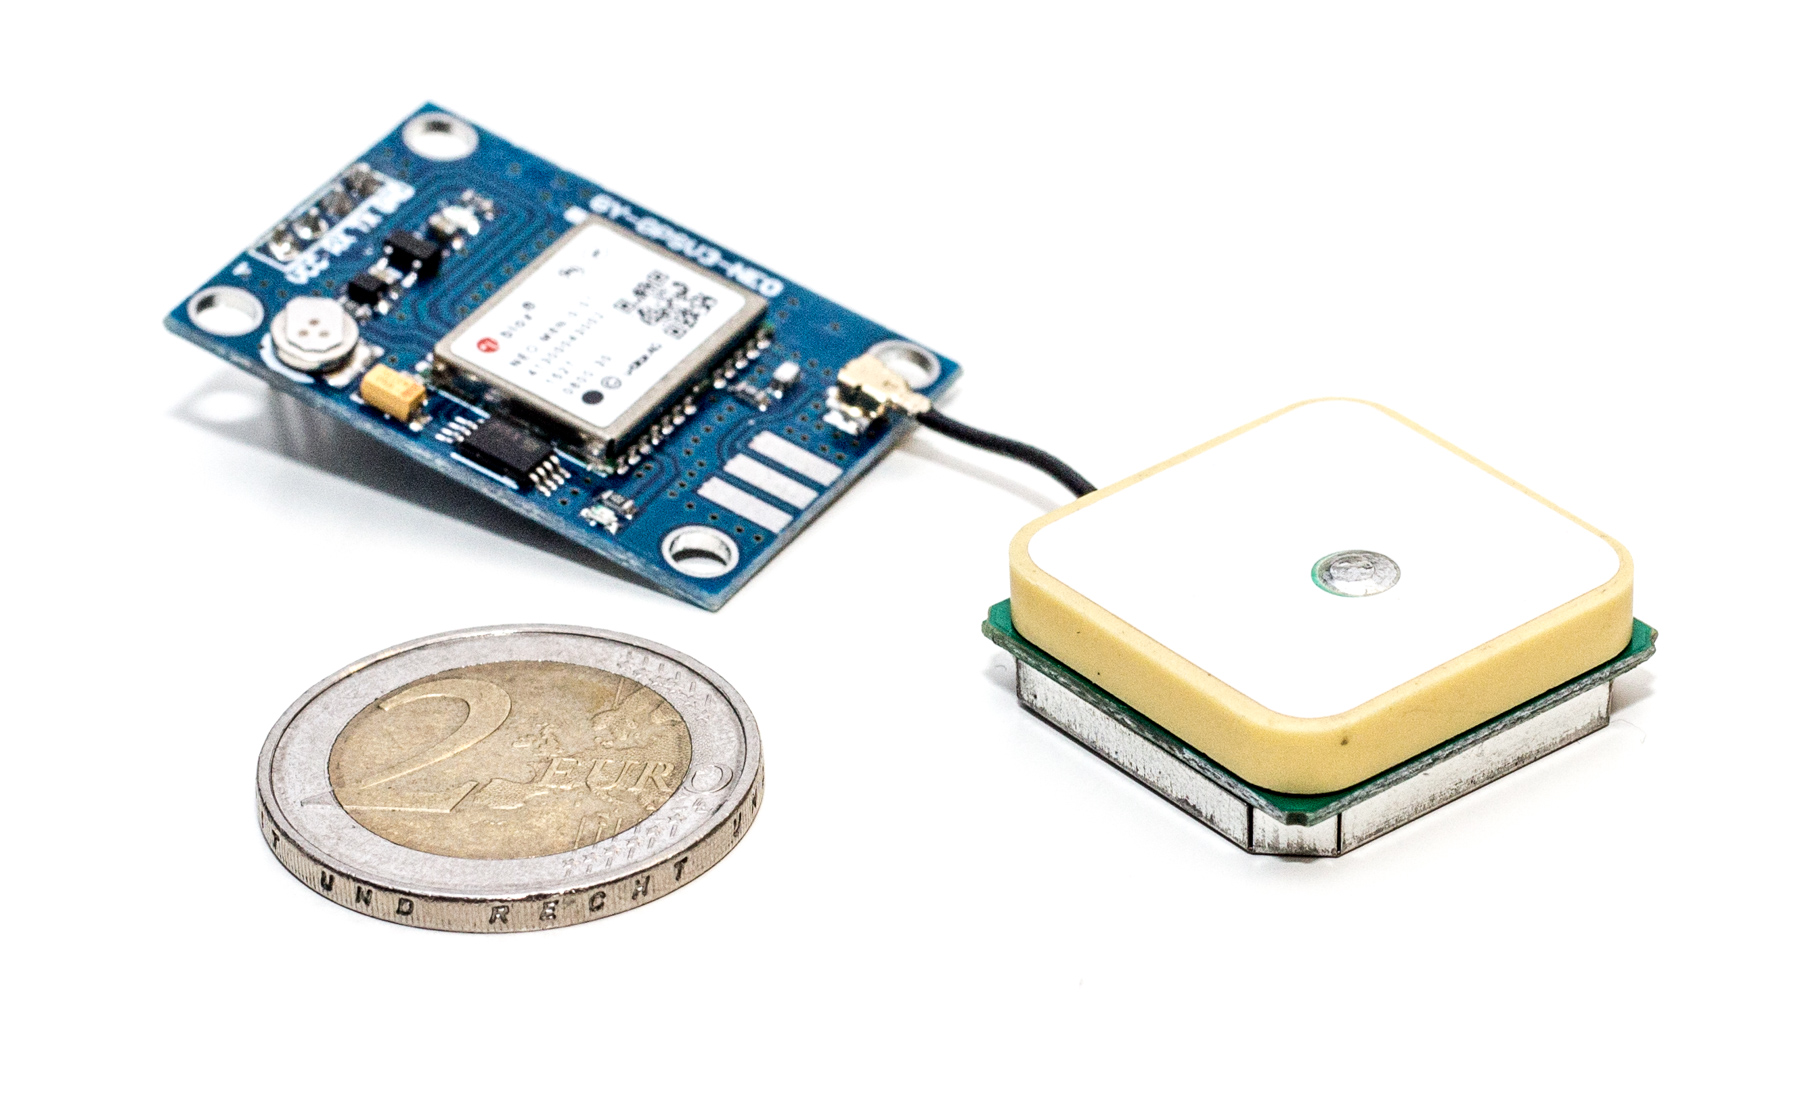
\includegraphics[width=0.7\textwidth]{./img/ublox.jpg}
 % vlp16.jpg: 0x0 pixel, 300dpi, 0.00x0.00 cm, bb=
 \caption{uBlox NEO-M8N, das Vorgängermodell NEO-6M mit PPS-Ausgang wurde verwendet (eigene Aufnahme)}
 \label{img:ublox}
\end{figure}

Die Übertragung der Daten des GNSS-Modules zum Laser\-scan\-ner erfolgt per serieller Schnittstelle über einen acht poligen Platinensteckverbinder. Bei dem vom Laser\-scan\-ner benötigten Übertragungsprotokoll handelt es sich um das standardisierte NMEA-Protokoll, welches mit einer Datenrate von \(9600~\frac{bit}{s}\) und einer Signalspannung zwischen 3 und 15 Volt übertragen wird. Der direkte Anschluss eines uBlox GNSS-Modules vom Typ NEO-6M brachte zunächst keinen Erfolg. Messungen mit einem Arduino (siehe \autoref{abb:oszi}) zeigten, dass das Signal des verwendeten GNSS-Moduls nicht dem im Datenblatt von \citet[S. 3]{vlpInterface} entsprach. Es zeigte sich, dass das Signal gedreht werden musste, da die Definition der Signalspannung verschieden war: Der Laser\-scan\-ner benötigte ein Signal, bei dem Logisch 1 mit einer Spannung von über 3 Volt \citep[S. 3]{vlpInterface} codiert ist (HIGH), beim GNSS-Modul entspricht  die höhere Spannung Logisch 0.

\begin{figure}
 \centering
 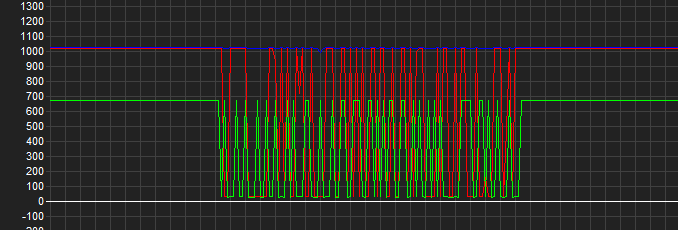
\includegraphics[width=0.7\textwidth]{img/oszi.png}
 % GNSS-Modul_Schaltplan_Entwurf.svg: 0x0 pixel, 300dpi, 0.00x0.00 cm, bb=
 \caption{Messung des Signals am uBlox NEO-6M (grün: Ausgangssignal; rot: Signal nach Nutzung eines Pegelwandler; 1000 Punkte entsprechen 5 Volt)}
 \label{abb:oszi}
\end{figure}

Um das Signal zu drehen wurde ein Integrierter Schaltkreis 74HC04 verwendet. Hierbei handelt es sich um ein Logikkonverter, der die HIGH- und LOW-Signale (Signal gegen Masse) tauscht. Der Laser\-scan\-ner versorgt das GNSS-Modull nur mit 5 Volt Spannung, der GNSS-Chip benötigt jedoch eine Spannung von 3,3 Volt. Hierfür wurde ein Spannungsregler verwendet, der die Spannung auf 3,3 Volt stabilisiert. Zur weiteren Stabilisierung wurden Kondensatoren eingesetzt. In Kombination mit dem Logikkonverter dient dieser auch als Pegelwandler. Die genaue Schaltung ist \autoref{abb:schaltplan} zu entnehmen.

\begin{figure}
 \centering
 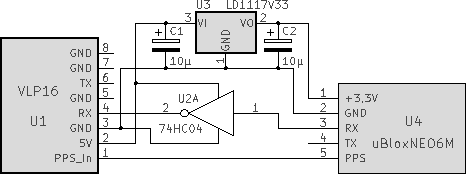
\includegraphics[width=0.8\textwidth]{img/schaltplanGnss.pdf}
 % GNSS-Modul_Schaltplan_Entwurf.svg: 0x0 pixel, 300dpi, 0.00x0.00 cm, bb=
 \caption{Entwurf der Schaltung zum Anschluss des GNSS-Modules an den Laser\-scan\-ner}
 \label{abb:schaltplan}
\end{figure}

\section{Steuerung im Betrieb}
\label{s:steuermodul}
Der Betrieb des Raspberry Pi erfolgt im Betrieb ohne Tastatur und Bildschirm. Daher ist es notwendig, eine alternative Benutzerschnittstelle zu implementieren. Ein großer Steuerbedarf ist nicht gegeben, so dass wenige Tasten zum Stoppen der Datenaufzeichung und zum Herunterfahren des Raspberry Pi ausreichend sind. Um auch eine Steuermöglichkeit zu implementieren, die im Flug genutzt werden kann, soll ein WLAN-Access-Point und ein simpler Webserver auf dem Raspberry Pi implementiert werden, der den Zugriff zum Beispiel über ein Smartphone oder Laptop ermöglicht.

\begin{figure}
 \centering
 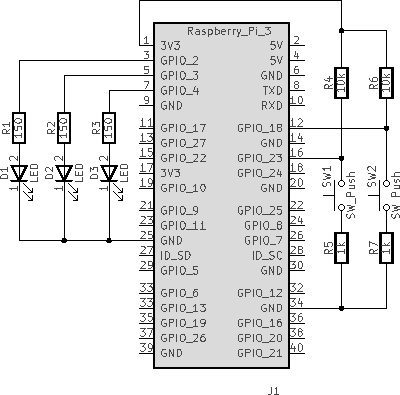
\includegraphics[width=0.7\textwidth]{img/schaltplanRasp.pdf}
 % GNSS-Modul_Schaltplan_Entwurf.svg: 0x0 pixel, 300dpi, 0.00x0.00 cm, bb=
 \caption{Entwurf der Schaltung für die Steuerung des Raspberry Pi}
 \label{abb:steuerung}
\end{figure}

\autoref{abb:steuerung} zeigt den Schaltplan des entwickelten Steuermodules. Dieses bietet mit drei Leuchtdioden und 2 Tastern die Möglichkeit, im Skript später einfache Anzeigen und Eingaben zu realisieren. Hierfür wurde eine Erweiterung auf Basis des GPIO-Portes des Raspberry Pi aufgebaut. Die zwei Taster sind über die beiden GPIO-Pins 18 und 25 erreichbar. Ohne Betätigung werden die Eingänge über die Pull-Up-Widerstände R4 und R6 auf ein High-Level gezogen. Durch Drücken des Tasters wird die Spannung über die Widerstände R5 und R7 auf ein Low-Level gezogen, welches durch das Pythonskript zur Laufzeit ausgelesen werden kann. Die Widerstände R5 und R7 dienen außerdem zur Strombegrenzung und als Sicherheit, falls die GPIO-Pins falsch geschaltet werden. In der weiteren Optimierung der Schaltung wurden die externen Pull-Up-Widerstände durch die interne, schaltbaren Pull-Up-Widerstände ersetzt. Dieses erwies sich vor allem bei der Nutzung ohne angestecktes Steuerungsmodul als vorteilhaft, da so auch ohne dieses Modul diese immer geschaltet sein können. Ansonsten könnten im Betrieb ohne Steuerungsmodul auftretende Spannungsschwankungen fehlerhafterweise zu einer Erkennung als Tastendruck führen.
Die drei Leuchtdioden wurden mit jeweils einem 150 Ohm Vorwiderstand direkt zwischen einem GPIO-Pin und Ground eingebaut. Durch Ansteuerung der GPIO-Pins lassen sich diese An- und Abschalten. Außer zum Schutz und Betrieb der LEDs verhindern die Vorwiderstände auch eine zu hohe Stromaufnahme aus den GPIO-Pins. Die genaue Belastbarkeit der Pins ist nicht dokumentiert, jedoch wird meist von einem Wert um 10mA bei 3,3 Volt gesprochen (zum Beispiel \citet{ekRaspPin}). Alternativ, bei Nutzung leistungsstärkerer LEDs könnten diese auch unter Nutzung eines Transistors geschaltet werden. Diese lassen mit einem geringen Steuerungsstrom höhere Ströme schalten.

\begin{equation}
\begin{aligned}
U_R &= U_{GPIO} - U_{LED} = 3,3V - 2,0V = 1,3V    && \left|\  \text{Benötigter Spannungsabfall} \right. \\
R &= \frac{U_R}{I_{LED}} = \frac{1,3V}{0,01A} = 130\Omega   && \left|\  \text{min. Vorwiderstand} \right. \\
\end{aligned}
\label{eq:vorwiderstand}
\end{equation}

\section{Platinenentwurf und -realisierung}
Nach dem Entwurf und Test der beiden Schaltungen aus \autoref{abb:schaltplan} und \autoref{abb:steuerung} auf einem lötfreien Steckbrett, soll diese Schaltungen zum späteren Einsatz an Bord des Multikopters als Platine mit verlöteten Bauteilen erstellt werden. Vorteile der gelöteten Schaltung sind in diesem Projekt ihre höhere Widerstandsfähigkeit gegen Vibrationen und Korrosion. Durch die Vibrationen im Flug könnten sich so Bauteile lösen und im schlimmsten Fall zum Kurzschluss und somit zur Zerstörung führen. Auch können die Kontakte zwischen den Federklemmen und den Bauteilen durch den Betrieb außerhalb von Gebäuden durch Luftfeuchtigkeit korrodieren und somit der Kontaktwiderstand höher werden, was zu Störungen führen kann.

Für den Prototyp soll die Schaltung von Hand aufgebaut und verlötet werden. Erst in der zukünftigen Entwicklung, wenn die Schaltung ausreichend erprobt wurde, könnte es sinnvoll sein, eine Platine ätzen zu lassen. Als Platine kommen daher vorerst nur vorgefertigte Layouts in Frage:

\begin{itemize}
 \item Lochrasterplatinen (Platine mit einzelnen Lötpunkten)
 \item Streifenrasterplatine (Lötpunkte sind in Streifen verbunden)
 \item Punktstreifenrasterplatine (Streifenrasterplatine, bei denen die Streifen regelmäßig, zum Beispiel alle 4 Lötpunkte, unterbrochen sind)
 \item spezielle Aufsteckplatinen für den Raspberry Pi
\end{itemize}

Da nur wenige Bauteile benötigt wurden, wurde eine Streifenrasterplatine gewählt. Bei einer solchen Platine sind alle Kontakte in einer Reihe mit einer Leiterbahn verbunden. Falls keine Verbindung gewünscht ist, kann diese Leiterbahn mit einem Messer oder ähnlichem unterbrochen werden. Da das Unterbrechen der Leiterbahn jedoch zeitaufwändig und fehlerträchtig ist, beispielsweise durch nicht vollständig getrennte Leiterbahnen, sollten diese beim Layouten der Platine möglichst vermieden werden. Auch sollte möglichst viele der benötigten Verbindungen durch diese Leiterbahnen erfolgen und möglichst wenig Drahtbrücken verwendet werden, die diese Leiterbahnreihen verbinden, da diese zusätzlichen Lötaufwand erfordern. Das endgültige Layout der Platine ist der \autoref{abb:platine} zu entnehmen.

\begin{figure}
 \centering
 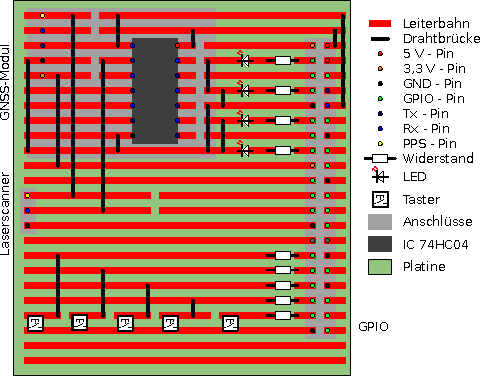
\includegraphics[width=0.9\textwidth]{img/platine.pdf}
 \caption{Layout der Lochstreifenplatine}
 \label{abb:platine}
\end{figure}

Beim Routing wurden noch einige Teile der Schaltung optimiert und versucht, einige Bauteile einzusparen, in dem zum Beispiel die Stromversorgung vom Raspberry Pi für den integrierten Schaltkreis und das GNSS-Modul verwendet wurden anstatt hierfür einen zusätzlichen Spannungswandler zu verwenden. Die Platinengröße wurde so gewählt, dass die Platine direkt auf den Raspberry Pi 2 oder 3 aufgesteckt werden kann. Der endgültige Schaltplan ist \autoref{abb:gesamtschaltung} zu entnehmen. Für die Taster wurden hier die internen Pull-Up-Widerstände genutzt, so dass hier zwei Widerstände eingespart werden konnten. Außerdem wurde der Datensendeport (Tx) vom GNSS-Modul an die serielle Schnittstelle des Raspberry Pi angeschlossen, so dass der Raspberry Pi nun auch ohne den Umweg über den Laser\-scan\-ner die Daten vom GNSS-Modul empfangen kann. Es wurde Platz für weitere LEDs und Taster freigelassen.

\begin{figure}
 \centering
 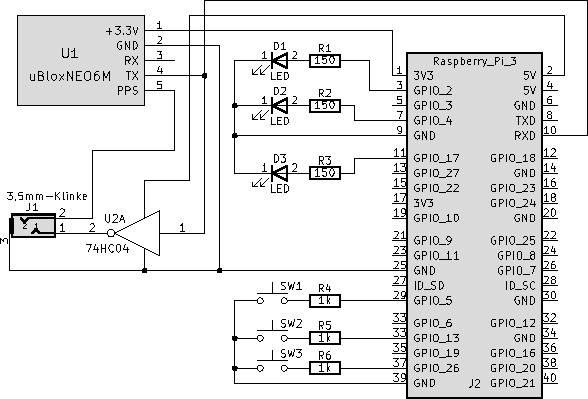
\includegraphics[width=1\textwidth]{img/schaltplanGesamt.pdf}
 \caption{Endgültiger Schaltplan}
 \label{abb:gesamtschaltung}
\end{figure}

\chapter{Theoretische Datenverarbeitung}
\label{c:datenverarbeitung}

\section{Verwendete Programmiersprachen}
\paragraph{Python}
Zur Realisierung der Programmierung wurde die Skriptsprache Python ausgewählt. Python bietet den Vorteil vergleichsweise kurzen und gut lesbaren Programmierstil zu fördern. Hierfür werden unter anderem nicht Klammern zur Bildung von Blöcken genutzt, sondern Texteinrückungen verpflichtend hierfür eingesetzt \citep[S. 13f]{python}. Die Struktur des Programms ist so schnell erfassbar. Außerdem ist es nicht notwendig, den Quellcode zu kompilieren. Er wird vom Interpreter direkt ausgeführt. So sind kurze Entwicklungszyklen ohne (zeit-)aufwändiges Kompilieren möglich. Änderungen und Anpassungen können schnell durchgeführt werden. Außerdem sind die Skripte größtenteils plattformunabhängig.

Python wurde in seiner ersten Version 1991 von Guido van Rossum freigegeben. Sein Ziel war es, eine einfach zu erlernende Programmiersprache zu entwickeln, die der Nachfolger der Sprache ABC werden sollte. Außerdem sollte die Sprache leicht erweiterbar sein und schon von Haus aus eine umfangreiche Standardbibliothek bieten. Python bietet mehrere Programmierparadigmen an, so dass je nach zu lösendem Problem objektorientiert oder strukturiert programmiert werden kann \citep[S. 14]{python}.

Die aktuelle Version von Python (Oktober 2017) ist die Version 3.6. Das Skript wurde unter Verwendung dieser Version entwickelt. Da sich viele Funktionen von der Version 2 zur 3 geändert haben, wurde auf die zuerst geplante Kompatibilität zu Python 2 verzichtet. Um Teile des Quellcodes als Python-Module auch in andere Skripte einfach einbinden zu können, aber auch den Quelltext übersichtlich zu halten, wurde der objektorientierte Programmierstil gewählt.

\paragraph{C++}
Ein großer Nachteil von Python ist die Ausführungsgeschwindigkeit. Daher wurden einzelne Teile des Quelltextes im Verlauf der Entwicklung in C++ umgeschrieben.
Bei C++ handelt es sich um eine objektorientierte Erweiterung der Programmiersprache C. C wurde 1972 von Dennis Ritchie entwickelt. Anfang der 1980er Jahre erweiterte Bjarne Stroustrup C zu C++. C++ hat zwar eine höhere Ausführungsgeschwindigkeit, dafür ist C++ jedoch nicht so leicht zu erlernen. \citep[S. 4f]{cpp}



\section{Datenlieferung vom Laser\-scan\-ner}
\label{ss:Datenlieferung}
Der Laser\-scan\-ner Velodyne VLP-16 liefert seine Daten als UDP-Netzwerkpakete in einem proprietären binären Datenformat. Diese Daten sind nicht direkt lesbar sondern müssen vor einer weiteren Nutzung aufbereitet und umgeformt werden. Dies soll mittels des in dieser Arbeit entwickelten Skriptes durchgeführt werden.

Ein Datenpaket (siehe \autoref{tab:datenmodell}) besteht jeweils aus einem Header von 42 Bytes, gefolgt von 12 Datenblöcken mit jeweils 32 Messungen, abgeschlossen von 4 Bytes, die den Zeitstempel angeben und 2 Bytes, die den eingestellten Scan-Modus zurückliefern. Jeder Datenblock enthält die aktuelle horizontale Ausrichtung des rotierenden Lasers und darauf folgend die Messwerte von zwei Messungen der 16 Laserstrahlen. Die genaue Horizontalrichtung zum Zeitpunkt der Messung muss aus den Horizontalrichtungen aus zwei auf einander folgenden Messungen interpoliert werden.

\begin{table}
\centering
\begin{tabular}{|lll|l|l|}
\hline
Header                                         &                                 
                &           & Netzwerk-Header  & 42 Bytes \\ \hline
\multicolumn{1}{|l|}{\multirow{7}{*}{Block 1}} &                                 
                & 0-1       & Flag             & 2 Bytes  \\ \cline{2-5} 
\multicolumn{1}{|l|}{}                         &                                 
                & 2-3       & Horizontalrichtung & 2 Bytes  \\ \cline{2-5} 
\multicolumn{1}{|l|}{}                         & 
\multicolumn{1}{l|}{\multirow{2}{*}{Messung 1}} & 4-5       & Entfernung       & 
2 Bytes  \\ \cline{3-5} 
\multicolumn{1}{|l|}{}                         & \multicolumn{1}{l|}{}           
                & 6         & Reflektivität    & 1 Byte   \\ \cline{2-5} 
\multicolumn{1}{|l|}{}                         & 
\multicolumn{1}{l|}{\multirow{2}{*}{Messung 2}} & 7-8       & Entfernung       & 
2 Bytes  \\ \cline{3-5} 
\multicolumn{1}{|l|}{}                         & \multicolumn{1}{l|}{}           
                & 9         & Reflektivtät     & 1 Byte   \\ \cline{2-5} 
\multicolumn{1}{|l|}{}                         & \multicolumn{4}{l|}{Messungen 3 
- 32}                                                     \\ \hline
\multicolumn{5}{|l|}{Block 2 - 12}                                               
                                                          \\ \hline
Time                                           & \multicolumn{1}{l|}{}           
                & 1200-1204 & Zeitstempel      & 4 Bytes  \\ \hline
Factory                                        & \multicolumn{1}{l|}{}           
                & 1205-1206 & Return-Modus     & 2 Bytes  \\ \hline
\end{tabular}

\caption{Aufbau der Daten des Netzwerkpaketes, nach \citet{vlpManual}}
\label{tab:datenmodell}
\end{table}

Der Laser\-scan\-ner sendet bei der Einstellung Dual Return, also der Rückgabe vom stärksten und letzten Echos pro Messung 
bis zu 1508 Pakete dieser Form pro Sekunde \citep[S. 49]{vlpManual}. Die Ausgangsdaten werden, bei einer Paketgröße von 1248 Bytes mit einer Datenrate von 1,8 MB/s empfangen (siehe \autoref{equ:Ausgangsrate}). Hierbei werden fast 600.000 Messwerte pro Sekunde übertragen (siehe \autoref{equ:MessungenPS}).

\begin{equation}
1508~\frac{\text{Pakete}}{\text{Sekunde}}~\cdot~12~\frac{\text{Datenbl\"{o}cke}}{\text{Paket}}~\cdot~
32~\frac{\text{Messungen}}{\text{Datenblock}}~=~579.072~\frac{\text{Datens\"{a}tze}}{\text{Sekunde}}
 \label{equ:MessungenPS}
\end{equation}

\begin{equation}
1508~\frac{\text{Pakete}}{\text{Sekunde}}~\cdot~1248~\frac{\text{Bytes}}{\text{Paket}}~=~1,79~\text{MB/s}
 \label{equ:Ausgangsrate}
\end{equation}

\section{Geplantes Datenmodell}
\label{s:datenmodell}
Die Daten des Laser\-scan\-ners sollen in einer einfach lesbaren Textdatei abgelegt werden. In der Nachbereitung sollen die Daten aus dieser Textdatei mit den Daten der inertialen Messeinheit und des GNSS-Empfängers verknüpft werden, um so die Daten georeferenzieren zu können. Als Verknüpfung bietet sich hier der Zeitstempel an. Die inertialen Messeinheit und der Laser\-scan\-ner können hierbei die Zeitdaten aus dem GNSS-Signal verwenden. Hierdurch sind hochgenaue Zeitstempel möglich. Die Zeitinformation bildet also einen wichtigen Schlüssel in den Daten. Als einfaches Textformat wurden durch Tabulator getrennte Daten, jeweils eine Zeile je Messung, gewählt. Folgende Daten sind in dieser Reihenfolge enthalten:

\begin{itemize}
 \item Zeitstempel in Mikrosekunden
 \item Richtung der Messung in der Rotationsebene in Grad
 \item Höhenwinkel zur Rotationsebene in Grad
 \item Gemessene Entfernung in Metern
 \item Reflektivität auf einer Skala von 0 bis 255
\end{itemize}

Problematisch ist bei diesem Datenmodell jedoch die benötigte Datenrate. Eine Datenzeile erfordert 29 Bytes und somit wird bei über einer halben Million Messungen pro Sekunde (siehe \autoref{equ:MessungenPS}) eine Datenschreibrate von mindestens 16 MB/s benötigt (siehe \autoref{equ:Datenrate}). Da das Schreiben nicht dauerhaft erfolgt, sollte die Datenrate bevorzugt deutlich höher sein.

\begin{equation}
579.072~\frac{\text{Datens\"{a}tze}}{\text{Sekunde}}~\cdot~29~\frac{\text{Bytes}}{\text{Datenzeile}}~=~16,02~\text{MB/s}
\label{equ:Datenrate}
\end{equation}

Erste Tests ergaben, dass diese Verarbeitungsgeschwindigkeit nicht mit dem Raspberry Pi erreicht werden konnte. Außerdem benötigen die Daten sehr viel Speicher. Daher wurde sich später für eine Hybridlösung entschieden (siehe \autoref{c:skript}).

\section{Weiterverarbeitung der Daten zu Koordinaten}
Die als Text gespeicherten Rohdaten sollen dann im Rahmen einer weiterführenden Arbeit zu Koordinaten umgewandelt werden. Zu dieser Umwandlung werden die Positionen des Laser\-scan\-ners mittels dem GNSS-Empfänger in der IMU und die Neigungsdaten aus der IMU verwendet. Die Neigungen werden dazu direkt mit den Winkeldaten verrechnet.

Bei der Berechnung ist jedoch zu beachten, dass der Ursprungsort der Entfernungsmessung zwar in der Drehachse des Laser\-scan\-ners liegt, jedoch der Ursprungsort der ausgesendeten Strahlen etwa 40mm in Strahlrichtung verschoben ist (siehe \autoref{img:strahlengang}). Bei der Streckenberechnung ist diese Strecke mit enthalten, jedoch kann zur Berechnung der Z-Komponente der lokalen Koordinaten nicht einfach der Höhenwinkel und die gemessene Strecke verwendet werden. Die lokalen Koordinaten berechnen sich somit nach der \autoref{equ:koordinaten}.

\begin{figure}
 \centering
 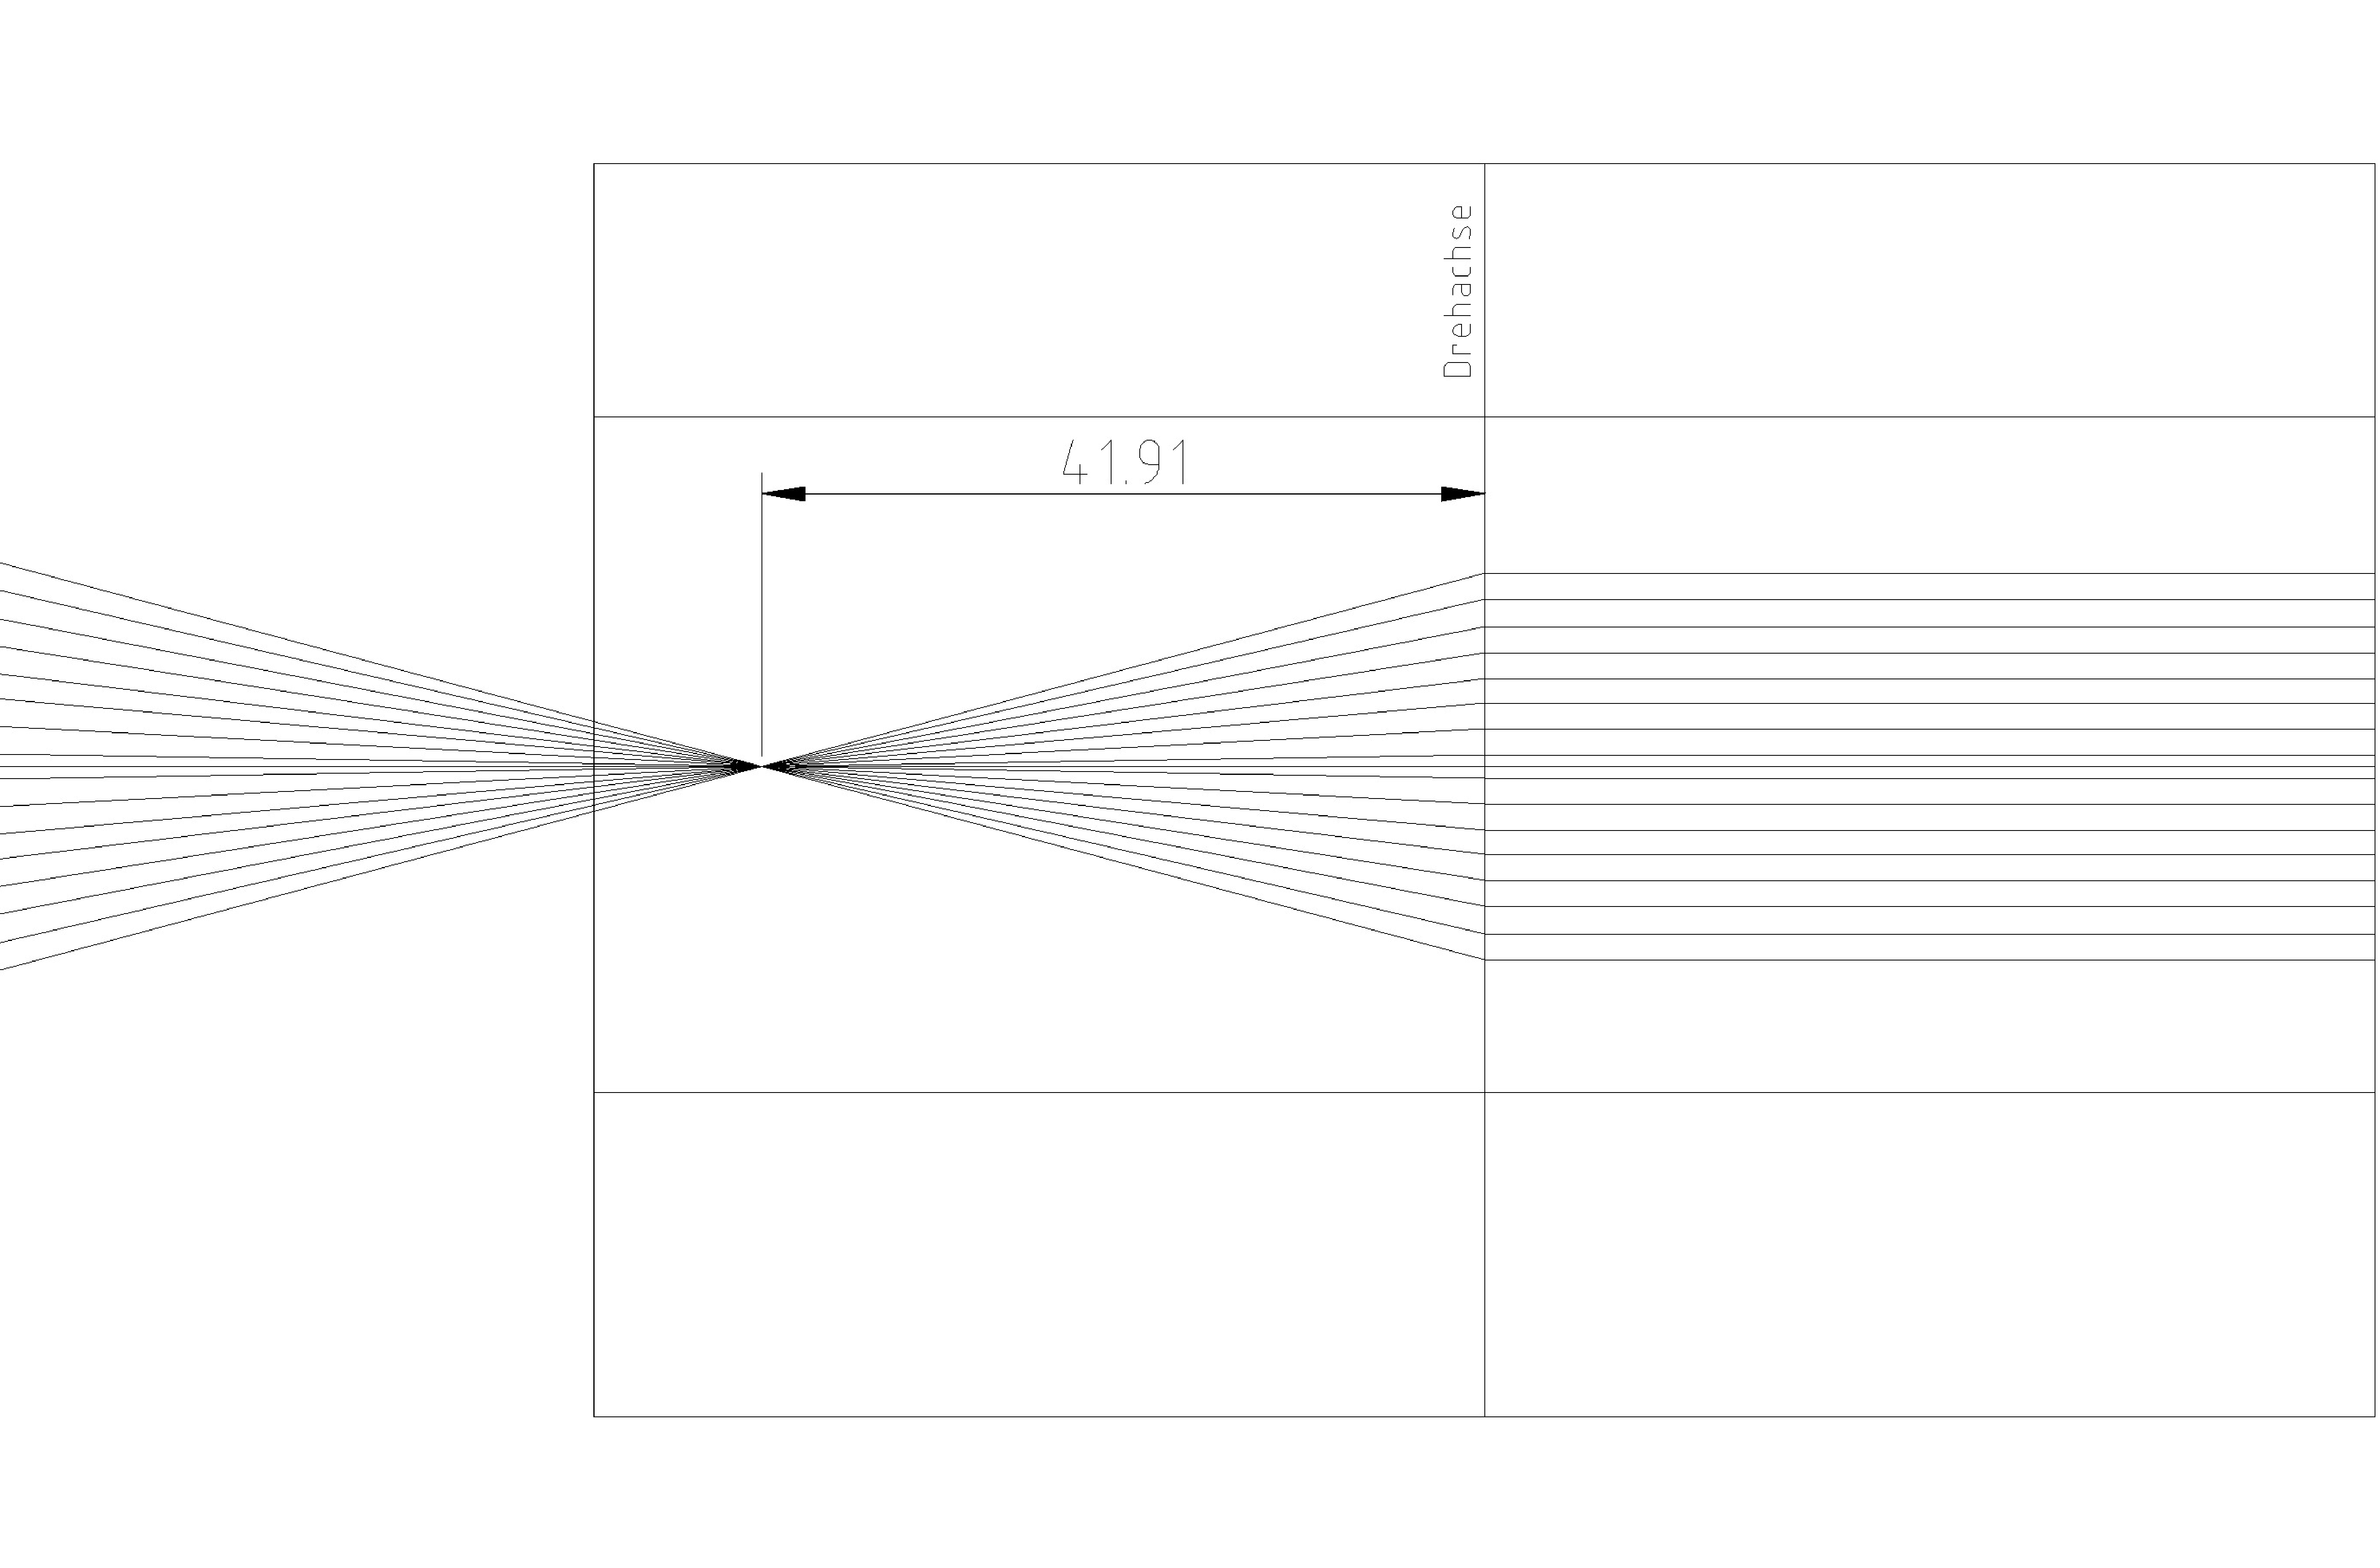
\includegraphics[width=0.7\textwidth]{./img/Strahlengang.png}
 % Strahlengang.eps: 0x0 pixel, 300dpi, 0.00x0.00 cm, bb=0 0 3066 4000
 \caption{Strahlengang im Laser\-scan\-ner VLP-16, Werte in Millimetern, nach 
\citet{vlpCAD}}
 \label{img:strahlengang}
\end{figure}

\begin{equation}
\begin{aligned}
h:&~\text{H\"{o}henwinkel}~(-15^\circ - 15^\circ) \\
r:&~\text{Horizontalrichtung}~(0^\circ - 360^\circ) \\
s:&~\text{Gemessene~Strecke} \\
\\
s_S &= s - 41,91~mm    		 && \left|\  \text{Schr\"{a}gstrecke nach dem Fokuspunkt} \right. \\
s_H &= s_S * \cos(h) + 41,91~mm  && \left|\  \text{Horizontalstrecke von der Drehachse} \right. \\
\\
X &= s_H \cdot \sin(r) && \left|\  \text{Y-Achse in Nullrichtung} \right. \\
Y &= s_H \cdot \cos(r) \\
z &= s_S \cdot \sin(h) \\
\end{aligned}
\label{equ:koordinaten}
\end{equation}

\section{Anforderungen an das Skript}
Aus den technischen Vorgaben ergeben sich dann folgende Funktionen, die das Skript aufweisen muss:
\begin{itemize}
 \item Rohdaten vom Scanner abrufen
 \item Zeit vom GNSS-Modul abrufen
 \item Steuerungmöglichkeit mittels Hard- und Software
 \item Umwandlung in eigenes Datenmodell
\end{itemize}

Der Ablauf der einzelnen Schritte ist oft abhängig vom Fortschritt anderer Schritte und Gegebenheiten. Daher wurden die benötigten, einzelnen Schritte vorerst als grober Ablaufplan skizziert. So hat der Raspberry Pi keinen eigenen Zeitgeber. Um die Dateien aber mit dem korrekten Zeitstempel zu versehen, ist daher eine aktuelle Uhrzeit notwendig - diese liefert das GNSS-Modul, welches am Laser\-scan\-ner angeschlossen ist, sofern ein GNSS-Fix besteht. Es muss also vor dem Erzeugen der Dateien auf ein gültiges GNSS-Signal gewartet werden. Der endgültige, vereinfachte Ablaufplan ist der \autoref{img:ablaufplan} zu entnehmen. 
\begin{figure}
 \centering
 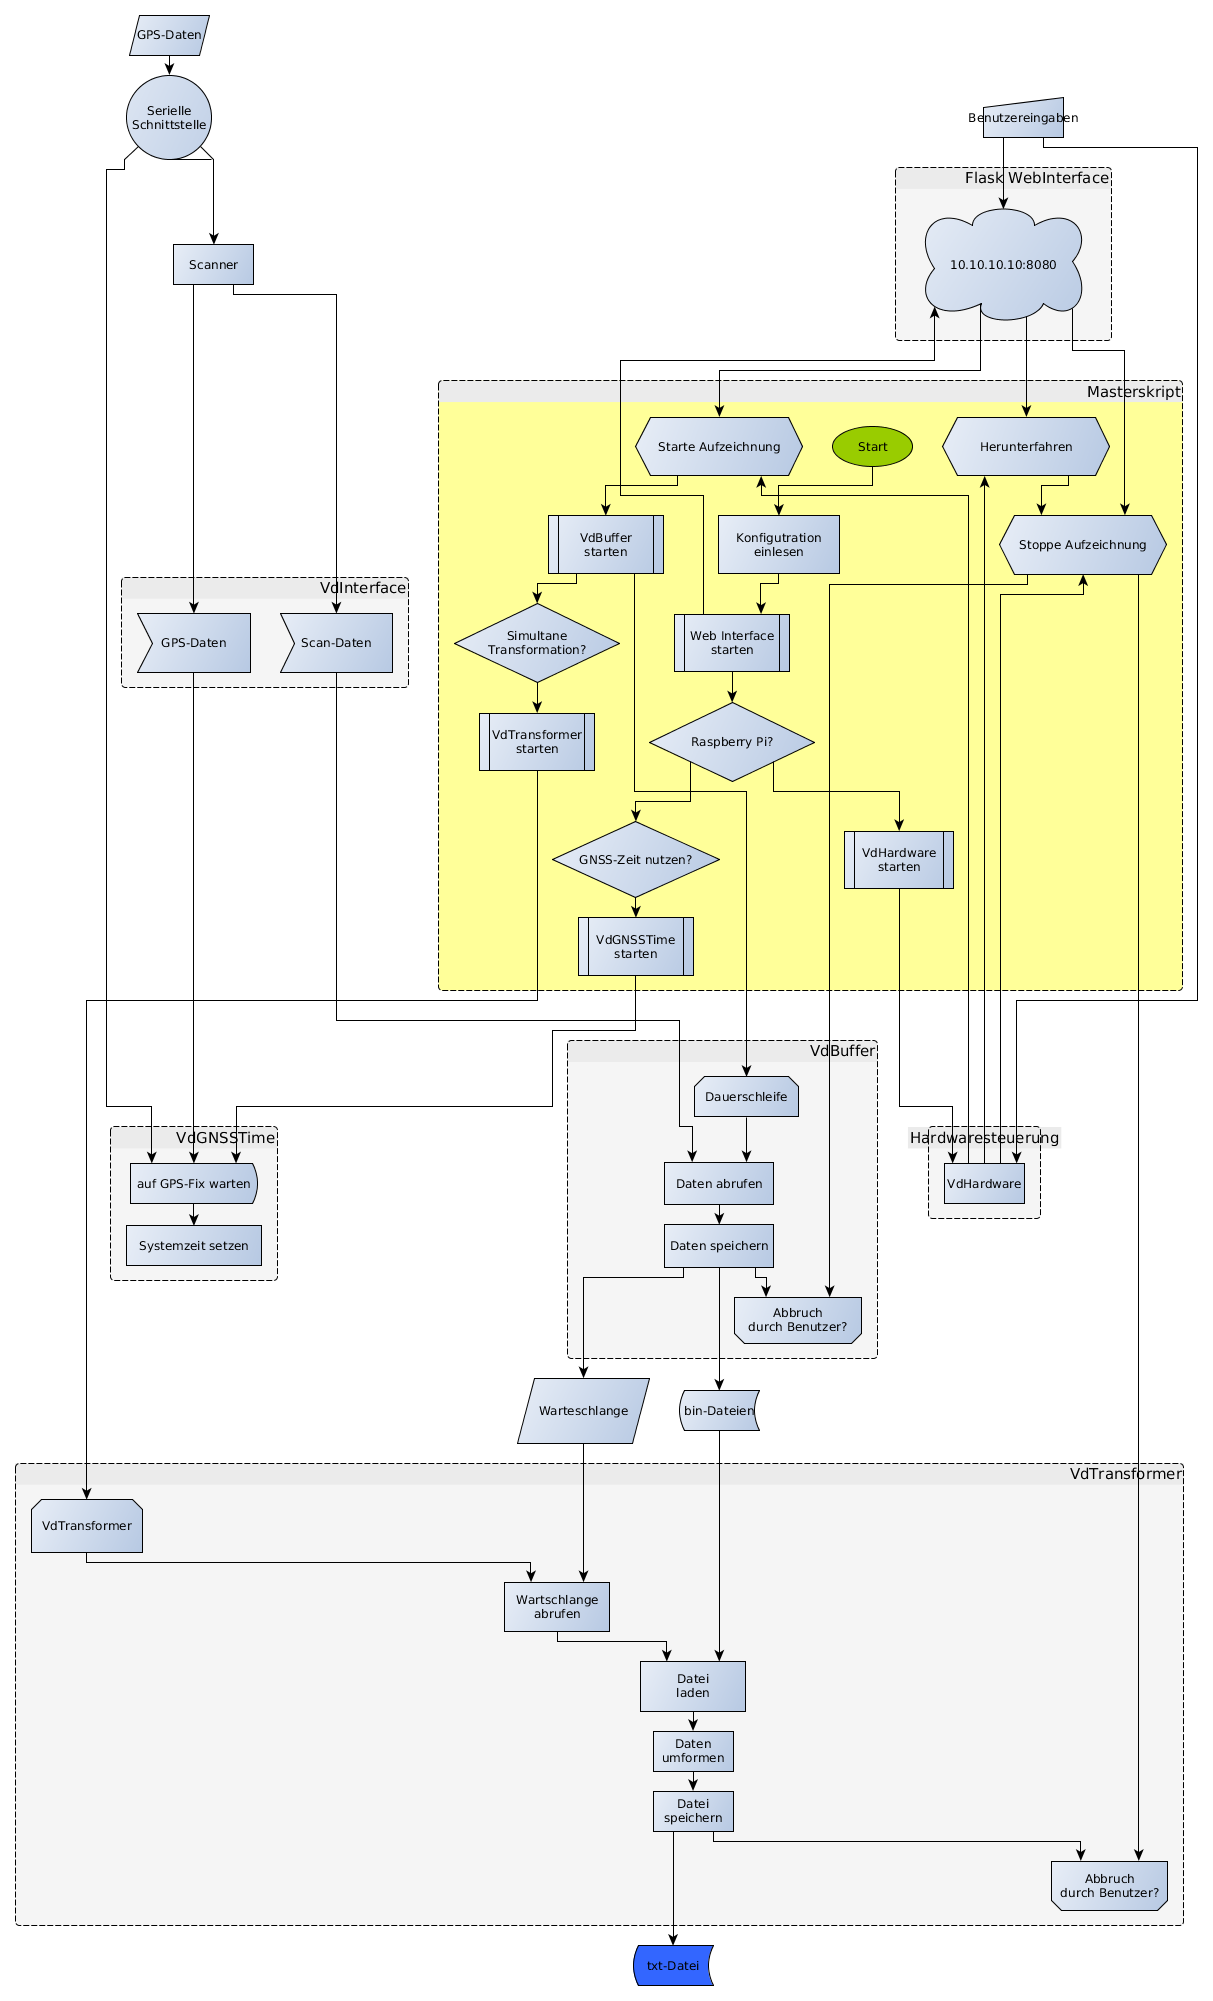
\includegraphics[width=0.8\textwidth]{./img/Ablaufplan.png}
 % Strahlengang.eps: 0x0 pixel, 300dpi, 0.00x0.00 cm, bb=0 0 3066 4000
 \caption{Vereinfachter Ablaufplan des Skriptes}
 \label{img:ablaufplan}
\end{figure}

\chapter{Entwicklung des Skriptes}
\label{c:skript}
\nocite{oopPython}
\nocite{uml}
\nocite{flask}

\section{Klassenentwurf}
Da das Skript objektorientiert programmiert werden soll, wurde zunächst mit Hilfe des Ablaufplanes aus \autoref{img:ablaufplan} die benötigten Klassen entworfen. Die endgültigen Klassen sind der \autoref{img:uml} zu entnehmen. Auf die genauen Funktionen der einzelnen Klassen wird im \autoref{s:klassen} eingegangen.

\begin{figure}
 \centering
 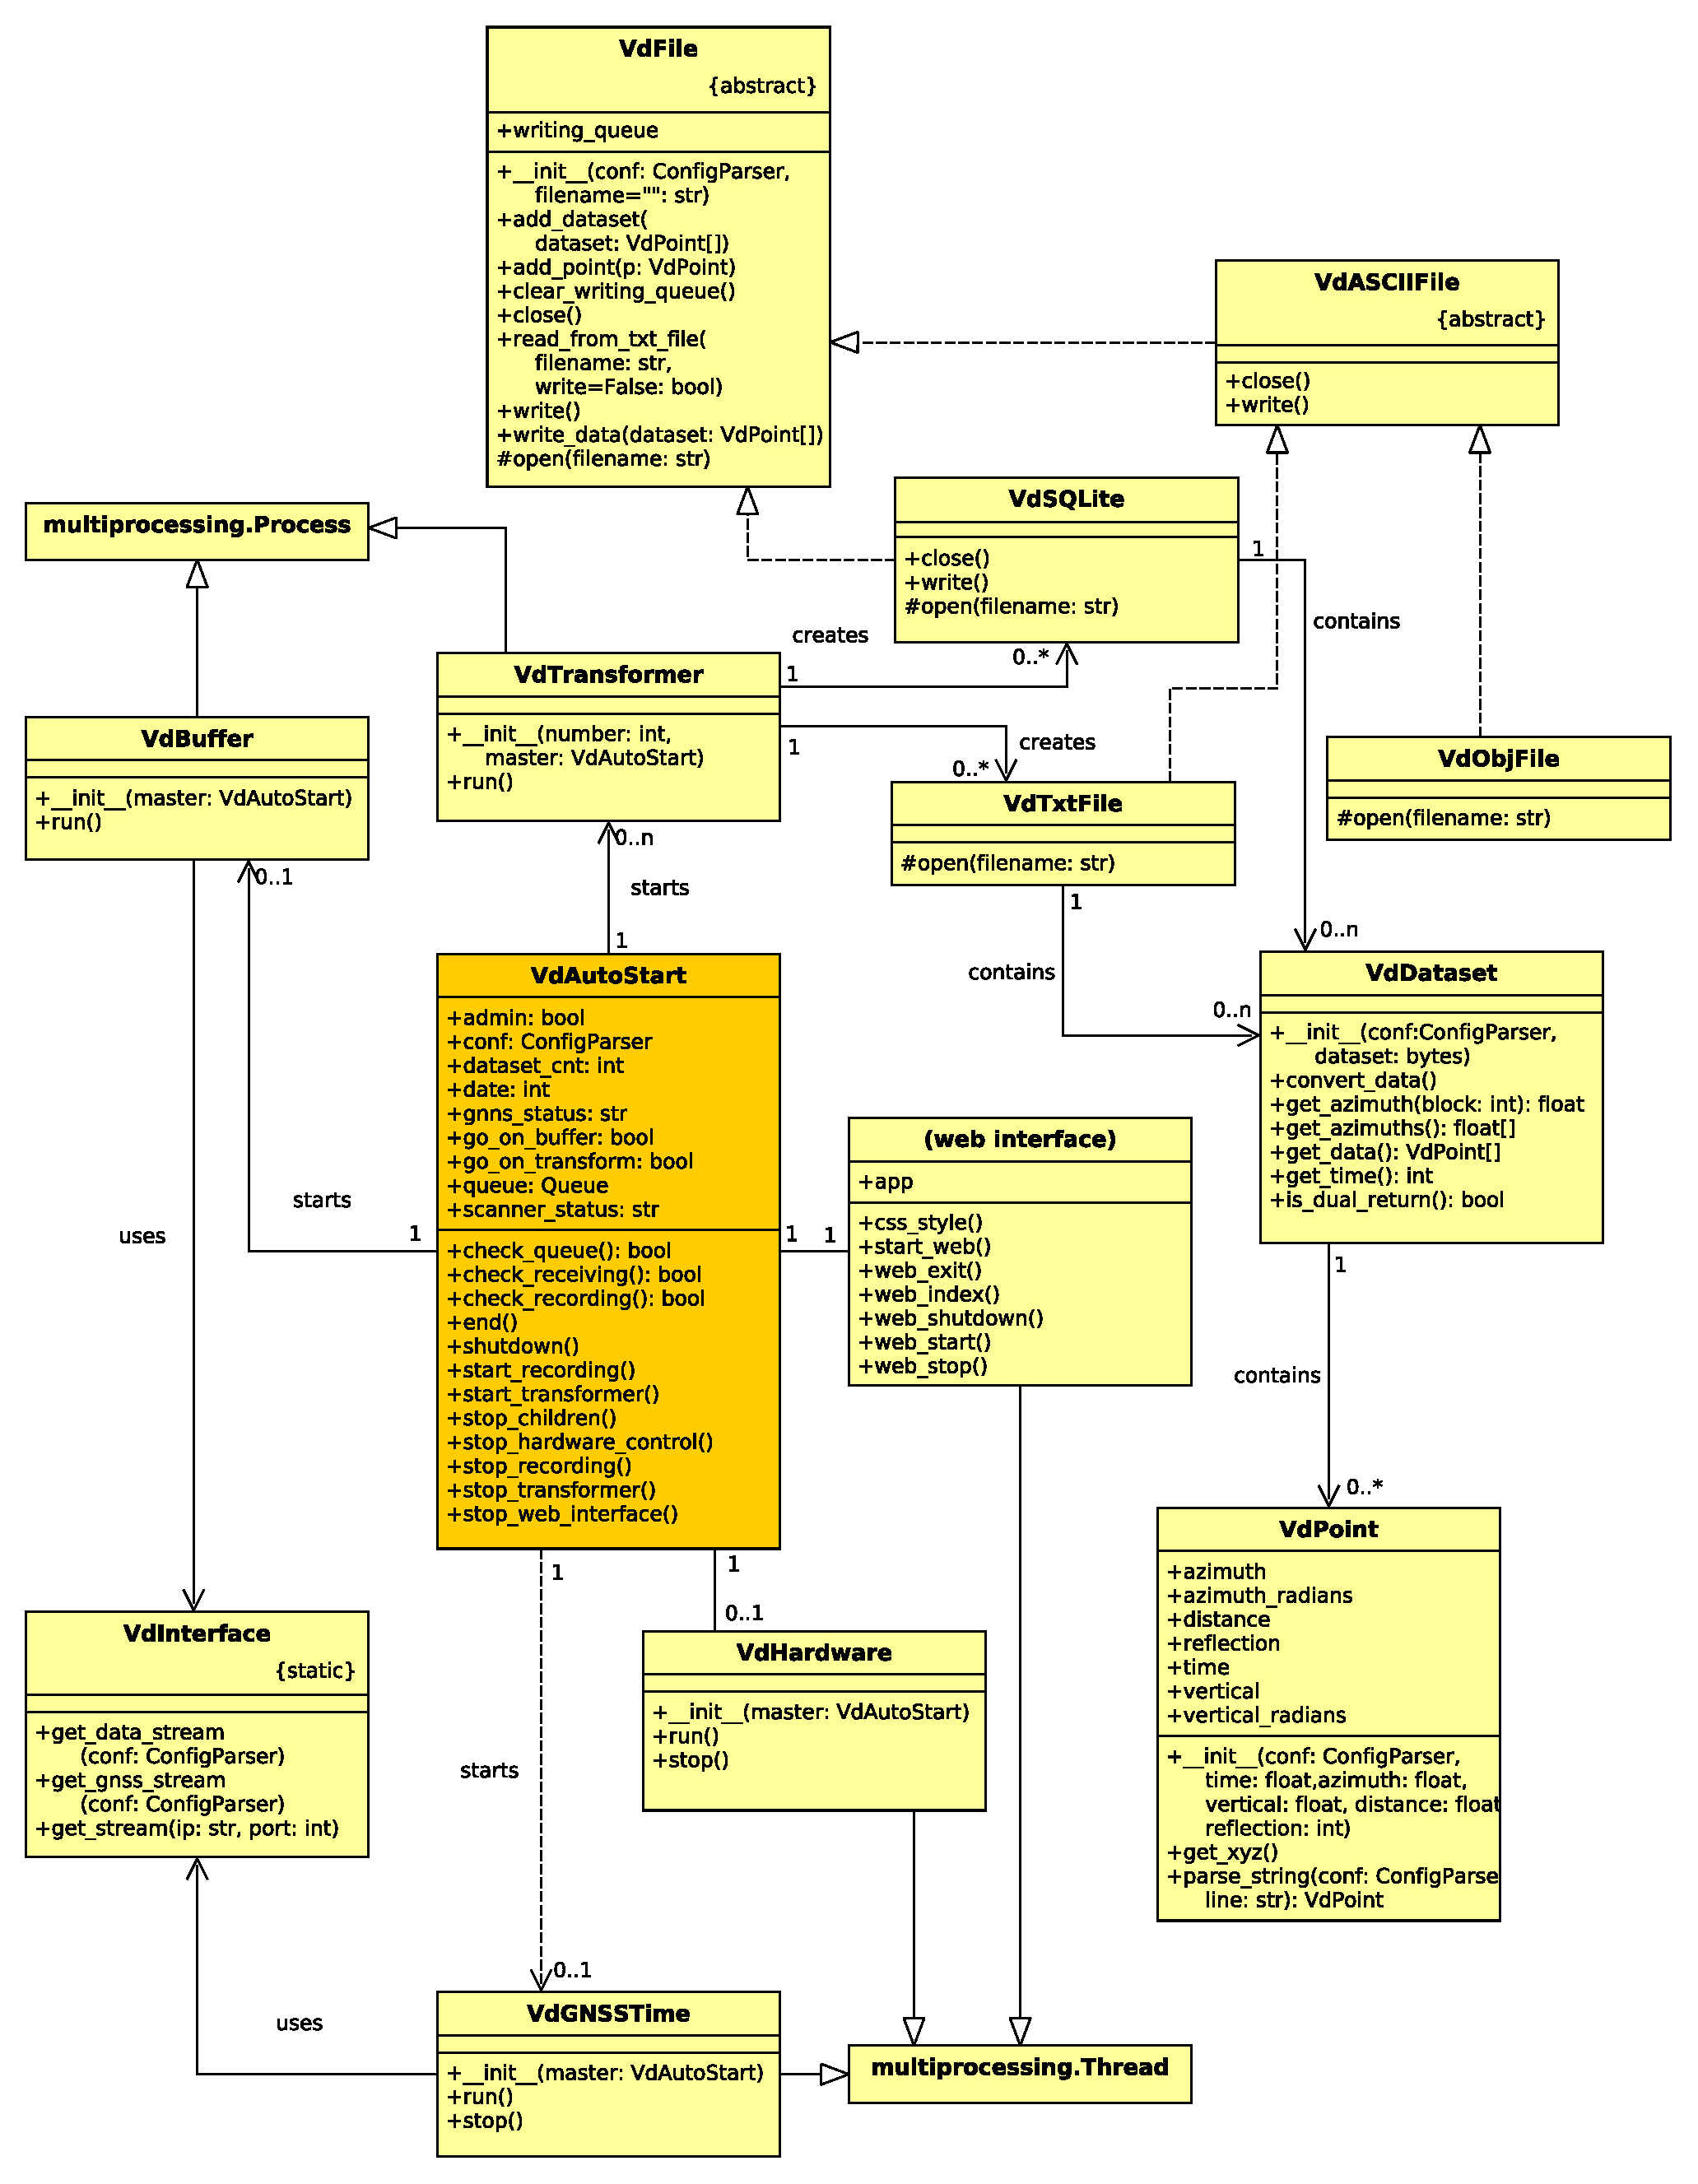
\includegraphics[width=1\textwidth]{./img/UML.pdf}
 % Strahlengang.eps: 0x0 pixel, 300dpi, 0.00x0.00 cm, bb=0 0 3066 4000
 \caption{UML-Klassendiagramm}
 \label{img:uml}
\end{figure}

\section{Evaluation einzelner Methoden}
Um eine einfache Fehlersuche zu ermöglichen, wurden die grundlegenden Funktionen in einzelnen Skripten entwickelt und geprüft. Diese kleineren Skripte haben den Vorteil, dass Fehler schneller eingegrenzt und auch schon früh konzeptionelle Fehler entdeckt werden können. In diesem Schritt wurde bemerkt, dass ein großes Problem die Geschwindigkeit der Datenverarbeitung ist. 

\paragraph{Datenempfang}
Die Verbindung zum Laser\-scan\-ner mittels Python-Socket funktionierte ohne weitere Probleme. Die binären Daten konnten zeitgleich abgespeichert werden.

\paragraph{Datentransformation}
Zunächst war es geplant, die Daten direkt in das in \autoref{s:datenmodell} vorgestellte Datenmodell umzuformen. Hierzu sollte der Empfang der Daten direkt eine Umformmethode starten. Die Versuche erfolgten zunächst mit dem im vorherigen Test aufgezeichneten Daten. Schon hier zeigte sich, dass die Umwandlung der aufgezeichneten Daten etwa das Fünffache der Mess- und Aufzeichnungzeit beanspruchte. Wie erwartet, brachte auch das direkte Einlesen der Daten vom Scanner keinen Erfolg. Es folgte ein Überlauf des Netzwerk-Buffers und somit der Verlust von Messdaten. Grund hierfür war hauptsächlich die benötigte Prozessorzeit. Die Nutzung einer schnelleren Datenspeicherung auf einer Solid-State-Disk mit einer Schreibrate von bis zu 300 MB/Sekunde änderte nichts an der Geschwindigkeit des Skriptes. Auch das Erzeugen eines neuen Threads für jeden empfangenen Datensatz war nicht erfolgsversprechend, da bis zu 1500 Threads pro Sekunde hierdurch gestartet wurden und das gesamte System überlastet wurde. Die Umformung musste daher von dem Datenempfang entkoppelt werden und das Skript für die Nutzung von Mehrkernprozessoren optimiert werden. Threads in Python laufen dennoch in einem Prozess und somit nur auf einem Prozessor. Es wurde das in \autoref{s:multikern} vorgestellte Multikern-Konzept erarbeitet.

\paragraph{Hardware-Steuerung}
Ein Tastendruck auf dem Steuerungsmodul (siehe \autoref{s:steuermodul}) sollte den Raspberry Pi zum Beispiel herunterfahren. Auch dieses Skript wurde getestet. Ein Problem hierbei war es, dass das Skript Administratorrechte (\code{root}) benötigte, um den Rechner herunterfahren zu können. Hierfür wurde jedoch eine Lösung gefunden, indem dem Nutzer \code{pi} die entsprechenden Rechte zum Herunterfahren gegeben wurden (siehe \autoref{s:root}). Eher zufällig zeigte sich aber noch ein anderes Problem: Sofern das Skript automatisch mit dem Start des Raspberry Pi gestartet wurde und das Steuermodul nicht angeschlossen war, fuhr der Raspberry Pi automatisch nach wenigen Sekunden Betrieb herunter. Da mit dem fehlenden Modul auch die Pull-Down-Widerstände fehlten, war der GPIO-Pin auf einem nicht definierten Zustand. Es kam dazu, dass er zufällig auf einem HIGH-Niveau war, welches als Drücken des Tasters interpretiert wurde. Nach Überschreiten der konfigurierten Haltezeit des Ausschalters von zwei Sekunden, wurde der Herunterfahrprozess gestartet. Um dieses Problem zu unterdrücken, wurde dem Skript zuerst eine vorherige Abfrage hinzugefügt, die beim Start überprüft, ob die beiden Taster sich auf einem Low-Niveau befinden, dass durch die beiden angeschlossenen Pull-Down-Widerstände erreicht wird. Falls dieses nicht der Fall ist, beendet sich die Hardwaresteuerung selbst\-stän\-dig. Im weiteren Verlauf der Entwicklung wurden dann jedoch das Signal gedreht und die internen Pull-Down-Widerstände des Raspberry Pi verwendet. Somit wurde diese Abfrage überflüssig.

\section{Multikern-Verarbeitung der Daten}
\label{s:multikern}
Da bei der Evaluation der einzelnen Methoden herausgefunden wurde, dass die Verarbeitungsgeschwindigkeit des Raspberry Pi für eine sofortige Transformation der Daten nach deren Eingang zu langsam ist, wurde ein Konzept erarbeitet, den hierdurch auftretenden Messdatenverlust zu unterdrücken.

Der Verarbeitung musste ein weiterer Buffer vorgeschaltet werden. Da aber das Abschalten des Raspberry Pi, zum Beispiel durch einen Verlust der Energieversorgung, nicht zu Datenverlusten führen sollte, konnten nicht die in Python integrierten Funktionen zur Datenzwischenspeicherung verwendet werden -- diese setzen zur Zwischenspeicherung auf den Arbeitsspeicher, der durch Stromverlust gelöscht wird. Das dauerhafte Schreiben auf die Festplatte -- im Fall des Raspberry Pi einer MicroSD-Speicherkarte -- führt aber zur weiteren Verzögerung. Es wurde daher eine Hybridlösung erarbeitet.

Die Arbeit wird nun auf mehrere Prozesse verteilt:
\begin{itemize}
 \item Start des Skriptes und Gesamtsteuerung in Prozess mit mittlerer Priorität (Klasse \code{VdAutoStart}, mit Threads für die Weboberfläche (Methode \code{startWeb()} in der Klasse \code{VdAutoStart}) und Hardwaresteuerung (Klasse \code{VdHardware})
 \item Sammeln der Daten mit höchster Priorität (Klasse \code{VdBuffer})
 \item Umformen der Daten durch mehrere Prozesse je nach Prozessorkernanzahl mit erhöhter Priorität (Klasse \code{VdTransformer})
\end{itemize}

Die Daten werden nun zuerst für wenige Sekunden im Arbeitsspeicher gesammelt. Sobald eine in der Konfiguration festgelegte Anzahl von Datensätzen zwischengespeichert wurde, werden diese im Dateisystem als binäre Datei abgelegt und der Dateiname in einer Warteschlange aus dem \code{multiprocessing}-Modul von Python (Klasse \code{Queue}) abgelegt. Die Prozesse zum Umformen der Daten fragen diese Warteschlange nun ab, verarbeiten jeweils eine binäre Datei und hängen die Ergebnisse an eine Ergebnis-Textdatei an. Die Dateinamen der binären Dateien, dessen Bearbeitung begonnen wurde, werden aus der Warteschlange entfernt. Nach dem Schreiben der umgeformten Daten werden die binären Dateien aus dem Dateisystem entfernt (abschaltbar). Damit die Umformer-Prozesse beim Schreiben nicht auf einander warten müssen, schreibt jeder Prozess in eine andere Ergebnisdatei. Diese können nach der Messung einfach zusammengefügt werden. Falls nun zum Beispiel die Stromversorgung unterbrochen wird, sind nun nur die Daten der letzten Sekunden verloren. Daten, die älter sind, sind entweder auch trotz Spannungsverlust als binäre Daten oder als Textdatei gespeichert. Durch ein Skript ist es möglich, den Umformerprozesses alleine zu starten und die restlichen, noch nicht gewandelten Daten umzuformen.

Durch dieses Prinzip stört eine stockende Datenumformung nicht die Aufzeichnung der Daten vom Scanner. Sofern der Raspberry Pi nicht die Geschwindigkeit der Umformung halten kann, werden einfach mehr binäre Dateien zwischengespeichert, die gegebenenfalls im Postprocessing umgewandelt werden können.

\section{Auslagerung der Transformation in C++}
Da auch bei Nutzung der kompletten Prozessorleistung des Raspberry Pi es nicht möglich war, die Daten zeitgleich zu transformieren und lange Nachbearbeitungszeiten auftraten, wurden weitere Ansätze geprüft. Am erfolgsversprechendsten war die Nutzung von C++ für diesen Teil. Die Programmiersprachen C und C++ sind bekannt dafür, dass sie sehr schnelle Ausführungszeiten bieten. Die Klassen, welche für die Transformation zuständig waren, wurden daher in C++ nachgebaut. Die Geschwindigkeit für die Umformung eines Testdatensatzes erfolgte in etwa der zehnfachen Geschwindigkeit. Diese Steigerung reicht aus, um bei Nutzung der vier Kerne des Raspberry Pi die Daten zeitgleich umzuformen. Der C++-Code wurde als eigenständiges Kommandozeilenprogramm erstellt. Somit ist es unabhängig vom Python-Code und kann auch selbständig verwendet werden, zum Beispiel zum späteren Umformen von Daten.
Die Pythonklasse \code{VdTransformer} wurde umschaltbar durch die Konfigurationsdatei um die Aufrufe des zusätzlichen Programmes erweitert. So kann je nach verwendeter Umgebung umgeschaltet werden zwischen der Umformung mittels Python (plattformunabhängig) und für verschiedene Plattformen kompilierter C++-Umformungen (ARM 32bit, Linux 64bit).

\section{Klassen}
\label{s:klassen}
Es folgt die Beschreibung der einzelnen Klassen. Auf die Konstruktor-Methoden \code{\_\_init\_\_()} wird nicht eingegangen, da hier meist nur Variablen deklariert werden.

\subsection{VdAutoStart (Python)}
Die Klasse \code{VdAutoStart} (siehe Anhang~\ref{a:vdAutoStart.py}) steuert den automatischen Start des Skriptes beim Hochfahren des Raspberry Pi. Sie ist verantwortlich für den korrekten Start der einzelnen Skriptteile in der richten Reihenfolge. Außerdem sind in der zugehörigen Datei auch alle Programmteile abgelegt, die nicht zu einer Klasse gehören, wie zum Beispiel der Startaufruf.
\todo{erweitern}

\paragraph{Flask-Webinterface app}
Die Weboberfläche zur Steuerung wird mit dem Modul \code{Flask} erzeugt. Die Weboberfläche wird durch die main-Methode in einem zusätzlichen Thread gestartet.
Die Weboberfläche ist entsprechend ihrem geplanten Einsatzzweck optimiert für die mobile Anzeige auf Smartphones, lässt sich aber auch vom Laptop bedienen. Die Oberfläche selbst nutzt nur HTML und CSS - ist also nicht zusätzlichen Skriptsprachen auf dem verwendeten Gerät abhängig. 

\subsection{VdInterface (Python)}
Die Klasse \code{VdInterface} (siehe Anhang~\ref{a:vdInterface.py}) übernimmt die Kommunikation mit dem Laser\-scan\-ner. Sie stellt die UDP-Socket-Verbindungen zum Datenstream des Scanners her.
\todo{zu kurz}


\subsection{VdHardware (Python)}
Die Klasse \code{VdHardware} übernimmt die Hardwaresteuerung des Raspberry Pi. Um etwas unabhängiger zu sein, stellt die Klasse einen eigenen Thread dar, der von der Klasse \code{VdAutoStart} je nach Hardware gestartet wird. Hierdurch werden die Abläufe des Hauptskriptes nicht durch die Abfrageschleifen der Hardwaresteuerung unterbrochen.

Bei der Initialisierung der Klasse werden die GPIO-Ports des Raspberry Pi entsprechend des Hardwaresteuerungsmodules aus \autoref{s:steuermodul} eingerichtet. Hierbei werden bei den Eingangsports die internen Pull-Up-Widerstände aktiviert. Beim Start des Threads wird dann zusätzlich ein Eventhandler für die Eingangspins eingerichtet, der entsprechende Funktionen zum Starten oder Stoppen der Aufzeichnung sowie zum Herunterfahren aufrufen. Desweiteren wird ein Timer aktiviert, der dafür sorgt, dass die LED-Anzeigen einmal sekündlich aktualisiert werden.

\subsection{VdPoint (Python / C++)}
Die \code{VdPoint}-Klasse stellt einen Messpunkt der Velodyne dar. Er nimmt als Attribute die Messdaten auf. Außerdem bietet die Klasse die Möglichkeit, die Messdaten in lokale kartesische Koordinaten mit dem Laserscanner als Ursprung umzurechnen. Dieses wird zum Beispiel bei der Erzeugung von OBJ-Dateien genutzt.
\todo{ergänzung?}

\subsection{VdDataset (Python / C++)}
Die Klasse \code{VdDataset} nimmt die Messdaten auf. Diese Klasse sorgt auch für das Interpretieren der binären Daten vom Laserscanner. Die Daten werden dann als \code{VdPoint}-Objekte in einer Liste gesichert. Durch die Übergabe der Daten an die Implementatierungen der Klasse \code{VdFile} können diese dann zum Beispiel als Datei gespeichert werden.

\subsection{VdFile und Subklassen (Python / C++)}
Bei der Klasse \code{VdFile} handelt es sich um eine abstrakte Klasse. Die Klasse stellt ein Interface da, das die Speicherung der umgewandelten Daten übernimmt. Die genauen Datenformate werden in Klassen festgelegt, die von ihr erben:

\paragraph{VdASCIIFile sowie VdTxtFile, VdObjFile und VdXYZFile}
Die abstrakte Klasse \code{VdASCIIFile} erweitert die Klasse \code{VdFile} um Funktionen, um ASCII-Dateien zu schreiben. \code{VdTxtFile} und \code{VdObjFile} implementieren dann die eigentlichen Dateiformate. Die Klasse \code{VdTxtFile} schreibt hierbei die Rohdaten als einfache Textdateien. \code{VdObjFile} formt die Rohdaten in lokale Koordinaten mit dem Ursprung im Standpunkt des Scanners um und speichert die Daten als OBJ-Datei. Das Dateiformat ist für das einfache Betrachten der Daten hilfreich. Es lässt sich als Punktwolke in vielen Programmen, wie zum Beispiel \code{MeshLab}, einlesen und darstellen. Im Zusammenhang mit der Vergleichsmessung aus \autoref{c:systemueberpruefung} wurde zusätzlich noch eine Klasse zur Implementierung von XYZ-Dateien erstellt. Hier werden die schon für die OBJ-Dateien aufbereiteten Daten in anderer Formatierung genutzt.

\paragraph{VdSQLite}
Die Klasse \code{VdSQLite} ermöglicht das Speichern der Rohdaten in einer SQLite-Datenbank-Datei. Das Format bietet sich zum einfachen Übertragen und Auswerten der Daten an. Alle Daten werden in einer Datenbank-Datei gesichert. Dies erleichtert das Einladen der Daten in weitere Skripte, zum Beispiel zum Durchführen von Berechnungen.

\subsection{VdBuffer}
Die Klasse \code{VdBuffer} übernimmt die Zwischenspeicherung der binären Rohdaten vom Laserscanner. Über die Klasse \code{VdInterface} wird eine Socketverbindung zum UDP-Port des Laserscanners hergestellt. Anschließend werden die Daten vom Socket in einer Variable gespeichert und regelmäßig in kurzen Intervallen als bin-Datei auf dem Speicher des Raspberry Pi abgelegt. Hierzu wird beim ersten Datenempfang ein Verzeichnis für die Messung angelegt. Nach dem Schreiben der Datei wird ihr Pfad in die Warteschleife für \code{VdTransformer} eingetragen.

\subsection{VdTransformer}
\code{VdTransformer} übernimmt die Umformung der als Datei gespeicherten binären Daten in \code{VdPoint}-Objekte. Um die Komponenten des Computersystems auszunutzen, werden durch \code{VdAutoStart} eine Instanz des Prozesses weniger gestartet, wie Prozessorkerne vorhanden sind - also auf dem Raspberry Pi als Vierkern-System 3 Prozesse der Klasse \code{VdTransformer} Sofern die Daten als ASCII-File gesichert werden sollen, wird für jede Instanz eine Datei erstellt, damit sich die Schreibprozesse nicht gegenseitig stören. Aus der Warteschlange wird jeweils eine bin-Datei ausgewählt, eingelesen und an die Klasse \code{VdDataset} übermittelt. Nachdem diese die Daten zu einer Liste von \code{VdPoint} umgewandelt hat, werden diese Daten an die Klasse \code{VdFile} übergeben. Diese schreibt dann je nach Einstellung in der Konfigurationsdatei die Daten im gewünschten Dateiformat. Nach dem erfolgreichen Schreibvorgang, wird die bin-Datei gelöscht (oder je nach Einstellungen verschoben).

\section{Steuerung des Skriptes}
Die grundlegenden Einstellungen erfolgen über die Konfigurationsdatei \code{config.ini}. Hier können Einstellungen zum Verhalten des Skript durchgeführt werden, aber auch die Parameter des Laserscanners angepasst werden. Die weitere Steuerung erfolgt über die Weboberfläche des Skriptes und des Laserscanner.

\chapter{Konfiguration des Raspberry Pi}
\label{c:konfig}

Als Grundlage wurde auf die MicroSD-Karte, die dem Raspberry Pi als Festplatte dient, das Betriebssystem Raspbian aufgespielt. Hierbei handelt es sich um ein Derivat von Debian GNU/Linux, das speziell auf die Hardware des Raspberry Pi angepasst wurde. Die aktuelle Version (Stand 27.10.2017) nennt sich Raspian Stretch. Für die Verwendung als Verarbeitungsgerät ohne angeschlossenen Display reicht die Variante ohne grafische Benutzeroberfläche aus (Raspbian Stretch Lite). Die Konfiguration des Raspberry Pi erfolgt vollständig über Konfigurationsdateien. In dieser Arbeit erfolgte die Konfiguration per Fernzugriff über SSH, einem Standard für das Fernsteuern der Konsole über das Netzwerk. Eine Konfiguration hätte aber auch mittels einem angeschlossenen Display und einer USB-Tastatur erfolgen können.

Die Änderungen der Konfigurationsdateien erfolgten mit dem vorinstallierten Editor \code{nano} unter Nutzung von Administratorrechten. Ein solcher Aufruf erfolgt zum Beispiel mit dem Befehl \code{sudo nano /pfad/zur/konfiguration.txt}. Nachfolgend müssen die betroffenen Programme oder sogar das komplette Betriebssystem neu gestartet werden. Der Neustart eines Services erfolgt zum Beispiel mit dem Aufruf \code{sudo service programmname restart}, der Neustart des Betriebssystems mit \code{sudo shutdown -r now}. Es empfiehlt sich, von allen zu ändernden Konfigurationsdateien Sicherungskopien anzulegen. Dies erfolgt zum Beispiel mit \code{sudo cp original.txt original.old.txt} (Kopieren) oder \code{sudo mv original.txt original.old.txt} (Verschieben, zum Beispiel zum Anlegen einer komplett neuen Datei). Auf diese Linux-Grundlagen wird im Folgenden nicht mehr eingegangen.

\section{Installation von Raspbian}
Die Installation von Raspbian erfolgt durch das Entpacken des Installationspaketes von der Website der Raspberry Pi Foundation auf einer leeren MicroSD-Karte mit dem Tool \code{Etcher}. Auf der nach dem Entpacken erzeugten boot-Partition wird eine leere Datei mit dem Namen \code{ssh} angelegt. Hierdurch wird sofort nach dem Start der SSH-Zugang über das Netzwerk zum Raspberry Pi ermöglicht, die IP-Adresse wird per DHCP, zum Beispiel von einem im Netzwerk vorhandenen Router, bezogen. Nach dem Einloggen zum Beispiel unter Linux mit dem Befehl \code{ssh pi@raspberrypi} und dem Passwort \code{raspberry}, kann mittels \code{passwd} das Passwort verändert werden.

% HafenCity

\section{Befehle mit Root-Rechten}
\label{s:root}
Linux erlaubt das Ändern der Zeit und das Herunterfahren über die Kommandozeile nur dem Administrator (\code{root}). Da es jedoch nicht empfohlen ist, Skripte als \code{root} auszuführen, muss hier eine andere Lösung gefunden werden, um den Skripten die Möglichkeit zu geben, den Raspberry Pi auf Tastendruck oder per Web-Steuerung herunterzufahren. Hierfür wurden dem normalen Nutzer (\code{pi}) die Rechte gegeben, einzelne Befehle  als Administrator ohne Passwortabfrage auszuführen. Diese Rechte können dem Nutzer durch Eintragung in die Konfigurationsdatei \code{/etc/sudoers} gegeben werden. Da eine fehlerhafte Änderung der Datei den kompletten Administratorzugang zum System versperren kann, wird die Datei mit dem Befehl \code{visudo} überarbeitet, der nach dem Editieren die Datei auf Fehler prüft. Die zusätzlichen Einträge in der Konfiguration sind dem \autoref{Lsudoers} zu entnehmen.\citep{sudoers}

\begin{lstlisting}[caption={Änderung der \code{/etc/sudoers}}, label={Lsudoers}]
# Cmnd alias specification
Cmnd_Alias VLP = /sbin/shutdown, /sbin/timedatectl

# User privilege specification
pi	ALL=(ALL) NOPASSWD: VLP
\end{lstlisting}

\section{IP-Adressen-Konfiguration}
Per Ethernet soll der Raspberry auf die IP-Adresse \code{192.168.1.111} konfiguriert werden, da diese IP-Adresse im Laser\-scan\-ner als Host eingestellt war und an diesen die Daten vom Scanner übertragen werden. Die IP-Adresse des Raspberry Pi im WLAN wurde fest auf die gut zu merkende Adresse \code{10.10.10.10} geändert, hierüber erfolgt später der Zugriff auf die Weboberfläche (siehe auch \autoref{tab:ipAdressen}).

\begin{table}
\centering
\begin{tabular}{l|r|r|l|}
\cline{2-4}
                                                    & Schnittstelle & \multicolumn{2}{c|}{IP-Adresse bzw. Bereich} \\ \hline
\multicolumn{1}{|l|}{Laser\-scan\-ner}                  & Ethernet      & 192.168.1.111        & statisch              \\ \hline
\multicolumn{1}{|l|}{\multirow{2}{*}{Raspberry Pi}} & Ethernet      & 192.168.2.110        & statisch              \\ \cline{2-4} 
\multicolumn{1}{|l|}{}                              & WiFi          & 10.10.10.10          & statisch              \\ \hline
\multicolumn{1}{|l|}{Client}                        & WiFi          & 10.10.10.100         & - 10.10.10.254        \\ \hline
\end{tabular}
\caption{IP-Adressen-Verteilung}
\label{tab:ipAdressen}
\end{table}

Die Konfiguration der IP-Adressen für den Raspberry Pi erfolgt in der Konfigurationsdatei \code{/etc/network/interfaces} (siehe \autoref{interfaces}. Um zukünftige Updates einfach zu ermöglichen, müssen die statischen IP-Einstellungen (Zeile 8-11) im Normalfall abgeschaltet werden und die DHCP Einstellungen (Zeile 13) aktiviert werden. \cite{accesspoint}

\begin{lstlisting}[caption={Konfiguration der \code{/etc/network/interfaces}}, label={interfaces}]
#localhost
auto lo
iface lo inet loopback

#Ethernet
auto eth0
## for Velodyne
iface eth0 inet static
	address 192.168.1.110
	netmask 255.255.255.0
	gateway 192.168.1.110
## for Internet etc. (DHCP)
# iface eth0 inet dhcp

allow-hotplug wlan0
iface wlan0 inet static
	address 10.10.10.10
	netmask 255.255.255.0
	network 10.10.10.0
\end{lstlisting}

Zur Konfiguration der dynamischen IP-Adressen der Clients im WLAN wird ein DHCP-Server eingerichtet. Ein solcher Server weißt neuen Geräten -- beziehungsweise welchen, die länger nicht im Netzwerk waren -- automatisch eine neue, unverwendete IP-Adresse zu. Hierdurch benötigen die Clients keine spezielle Konfiguration und ihre IP-Einstellungen können auf dem üblichen Standardeinstellungen verbleiben (automatische IP-Adresse beziehen). Als DHCP-Server wird hier das Paket \code{dnsmasq} verwendet. Außer dem DHCP-Server bietet dieses Paket auch einen DNS-Server, der es erlaubt, den Geräten auch einen Hostname zuzuweisen. So wäre der Zugriff zum Beispiel über den Hostname raspberry.ip anstatt durch Eingabe der IP-Adresse möglich.

Die Konfiguration des DHCP-Servers ist vergleichsweise einfach und benötigt nur das verwendete Netzwerk-Interface, hier wlan0, den zu nutzenden IP-Bereich, die Netzmaske und die Zeit, nach der eine IP-Adresse an ein anderes Gerät vergeben werden darf, die sogenannte Lease-Time (siehe \autoref{dnsmasq}). \cite{accesspoint}

  
\begin{lstlisting}[caption={Konfiguration der \code{/etc/dnsmasq.conf}}, label={dnsmasq}]
interface=wlan0
  dhcp-range=10.10.10.100,10.10.10.254,255.255.255.0,24h
\end{lstlisting}

\section{Konfiguration als WLAN-Access-Point}
Um einen Zugriff auf die Python-Weboberfläche des Skriptes und die Konfiguration des Laser\-scan\-ners zu ermöglichen, soll der Raspberry Pi selbst als WLAN-Access-Point fungieren. Hierzu wurde das Paket \code{hostapd} verwendet. Zur Konfiguration werden die Einstellungen in die Datei \code{/etc/hostapd/hostapd.conf} geschrieben. \cite{accesspoint}

\begin{lstlisting}[caption={Konfiguration der \code{/etc/hostapd/hostapd.conf}}, label={hostapd}]
# WLAN-Router-Betrieb

# Schnittstelle und Treiber
interface=wlan0
#driver=nl80211

# WLAN-Konfiguration
ssid=VLPinterface
channel=1
hw_mode=g
ieee80211n=1
ieee80211d=1
country_code=DE
wmm_enabled=1

#WLAN-Verschluesselung
auth_algs=1
wpa=2
wpa_key_mgmt=WPA-PSK
rsn_pairwise=CCMP
wpa_passphrase=raspberry
\end{lstlisting}

\section{Autostart des Skriptes}
Damit das Skript vor der Messung mittels SSH-Zugang gestartet werden muss, wurde das Skript in den Autostart des Raspberry Pi eingetragen. Hierdurch erfolgt der Start des Skriptes unmittelbar nach dem Hochfahren des Betriebssystems. Durch die Nutzung des Befehls \code{su} wird der Befehl als Nutzer \code{pi}, also ohne Administratorrechte gestartet. Durch Weglassen von \code{su pi -c} kann dieser auch als Administrator gestartet werden. Dies hat jedoch sicherheitstechnische Nachteile, dafür können dann Prioritäten der Befehle gesetzt werden.

\begin{lstlisting}[caption={Startskript startVLP.sh}, label={startskript}]
su pi -c "python3 VdAutoStart.py"
exit 0
\end{lstlisting}

Der Pfad zur dem Startskript wurde dann in der Autostart-Konfigurationsdatei \code{/etc/rc.local} eingetragen.

\section{Einrichtung als Proxy}
Zusätzlich ist es sinnvoll, den Raspberry Pi auch als Proxy einzurichten. So lässt sich dann über die WLAN-Schnittstelle des Raspberry Pi auf die Konfigurationswebseite  des Laserscanners zugreifen, um Einstellungen des Scanners mobil zu ändern.

\todo{zu Ende schreiben}

\chapter{Systemüberprüfungen}
\label{c:systemueberpruefung}
Nachdem bei der Systemkonfiguration bisher auf die Angaben aus Handbüchern und Anleitungen vertraut wurde, sollte zusätzlich die Genauigkeit von einigen Systemkomponenten überprüft werden. Hierfür wurde einmal die Messgenauigkeit des Scanners ausgewählt sowie die Genauigkeit der Zeitangaben der GNSS-Systeme. Die Genauigkeit des GNSS und der in Zusammenhang mit der IMU zu berechnenden Trajektorie hatte bereits \citet{wilken} in seiner Bachelorthesis untersucht.

\section{Untersuchung der Gleichzeitigkeit von PPS-Signalen von verschiedenen GNSS-Empfängern}
Für die Synchronisierung der Daten des Laser\-scan\-ners und der inertialen Messeinheit wurden zwei verschiedene GNSS-Empfänger verwendet. Der für den Einbau in Consumer-Geräte gedachte uBlox-Chip, der am Raspberry Pi und am Laser\-scan\-ner verwendet wird, ist leichter, unabhängiger und einfacher zu realisieren als die Übernahme der Daten mittels Adapterkabeln von der inertialen Messeinheit. Voraussetzung hierfür ist jedoch, dass beide Signale wirklich gleichzeitig erzeugt werden. Um dies zu überprüfen, soll das PPS-Signal (Impulssignal im Sekundentakt) von beiden Messsystemen mit einem Arduino überprüft werden.
Am Arduino werden hierzu an zwei digitalen Eingängen die PPS-Anschlüsse der GNSS-Empfänger angeschlossen. Ein Skript \todo{skript} misst dann die Zeit zwischen den beiden Signalen. Diese Messungen werden dann mehrfach hintereinander sowie nach einem Neustart der Systeme durchgeführt. Hiermit soll überprüft werden, ob bei einem Neustart der Messung sich die Zeitdifferenz ändert beziehungsweise überhaupt eine Zeitdifferenz dann entsteht.


\section{Messgenauigkeit des Laser\-scan\-ners im Vergleich}
Um die Strecken und Winkelmessung des Laserscanners zu überprüfen, wurden an zwei Standpunkt an der Hafencity Universität jeweils Scans mit dem Velodyne VLP-16 durchgeführt. Das erste Messszenario fand etwa 20 Meter von einer weißen, rauen und ebenen Fassade (Verputztes Wärmedämmverbundsystem) statt. Hier wurden zum Vergleich mit einem terrestrischem Laserscanner Zoller+Fröhlich Imager 5010 der Messaufbau komplett von zwei Standpunkten aus gescannt. Hierbei sollte vor allem die Streckenmessung überprüft werden. Das zweite Messszenario fand in der Tiefgarage der Universität statt. Sie ist etwa 100 Meter lang und von vielen eckigen Säulen durchzogen. Hier bot es sich an, die Widerholungsgenauigkeit in Strecke und Richtung des Laserscanners zu überprüfen und zusätzlich boten die Säulen verschiedene Entfernungen und Auftreffwinkel. Die meisten Oberflächen bestanden hier aus weiß gestrichenen Beton.

\paragraph{Auswertung der Daten von Velodyne VLP-16}
Die Daten des Velodyne VLP-16 wurden mit dem in dieser Arbeit entwickelten Skript aufgezeichnet und umgewandelt. Da hierbei auffiel, das einige Programme besser mit XYZ-Dateien umgehen können, wurde das Klassenmodell um dieses Dateiformat erweitert.

\begin{figure}
 \centering
 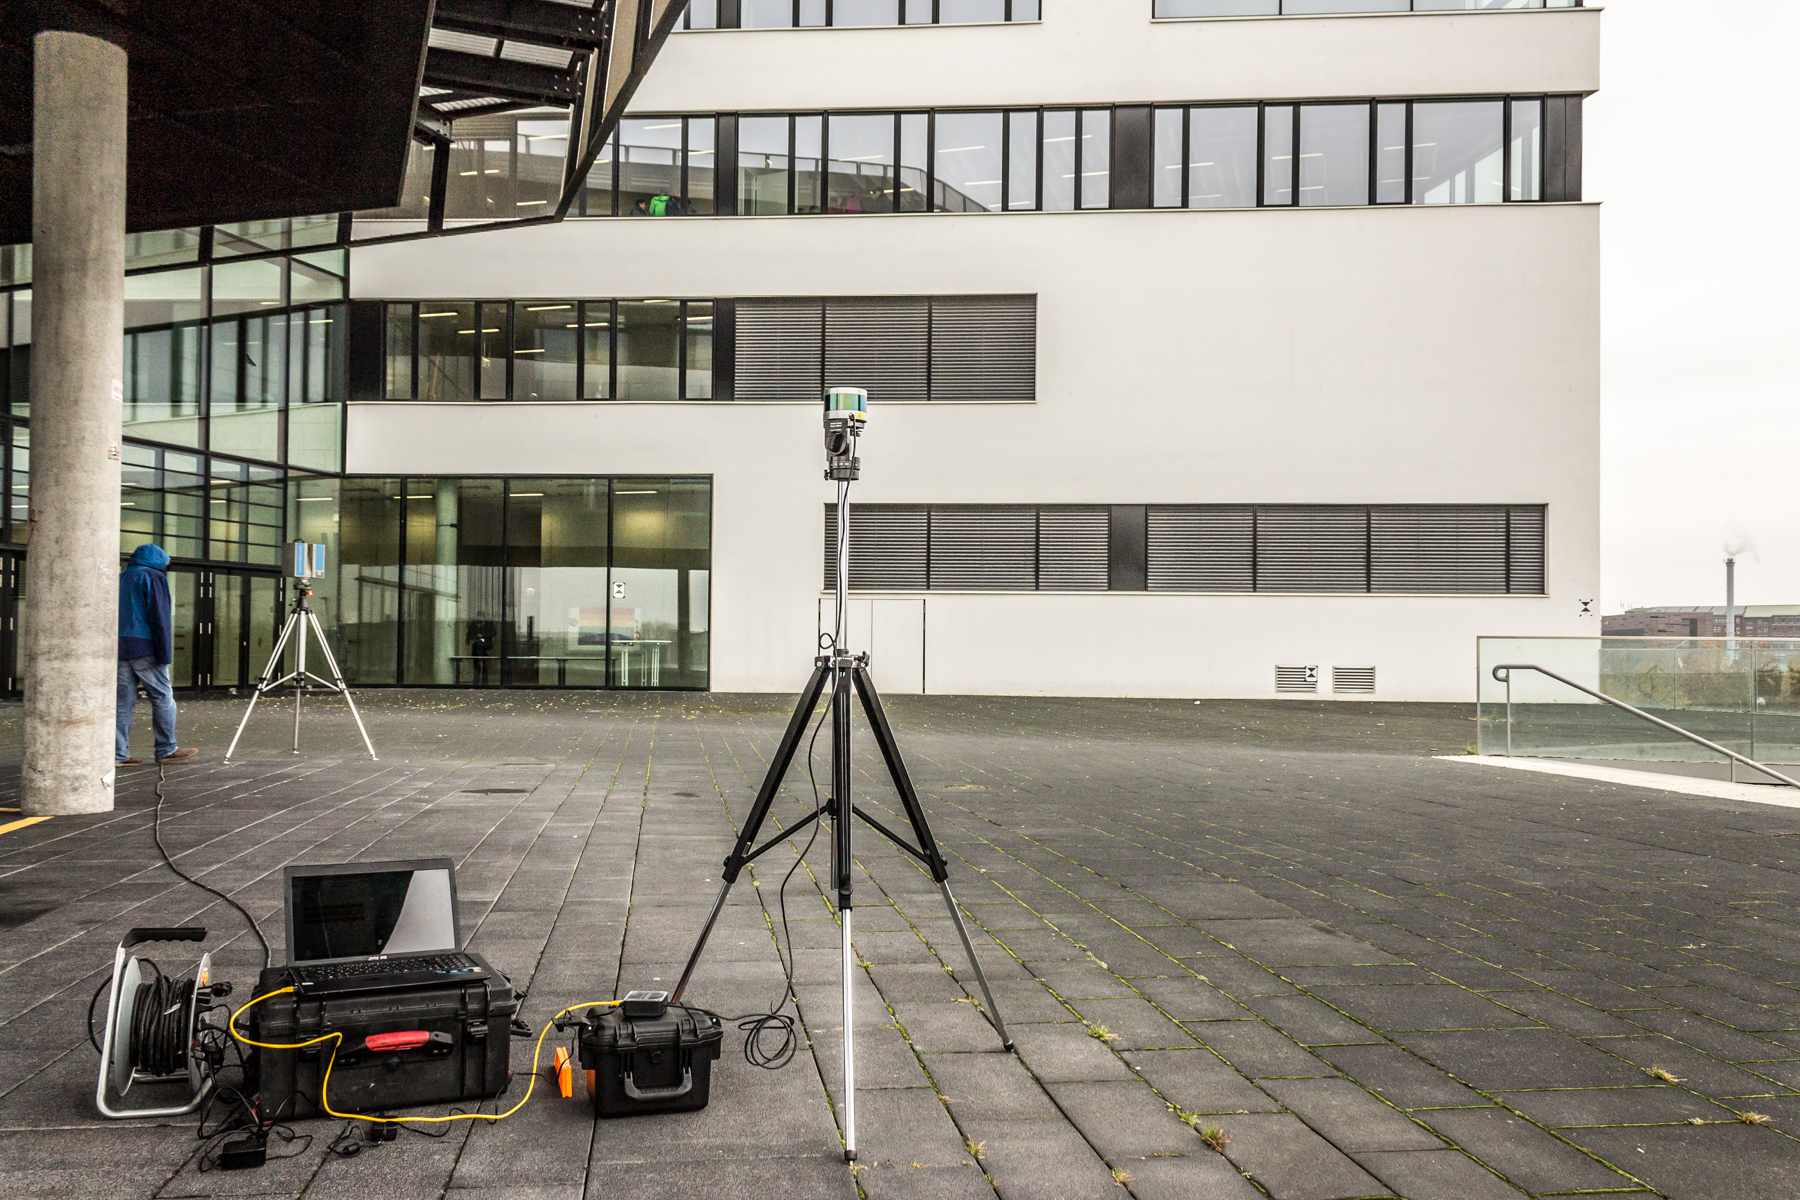
\includegraphics[width=0.45\textwidth]{./img/fassade.jpg}
 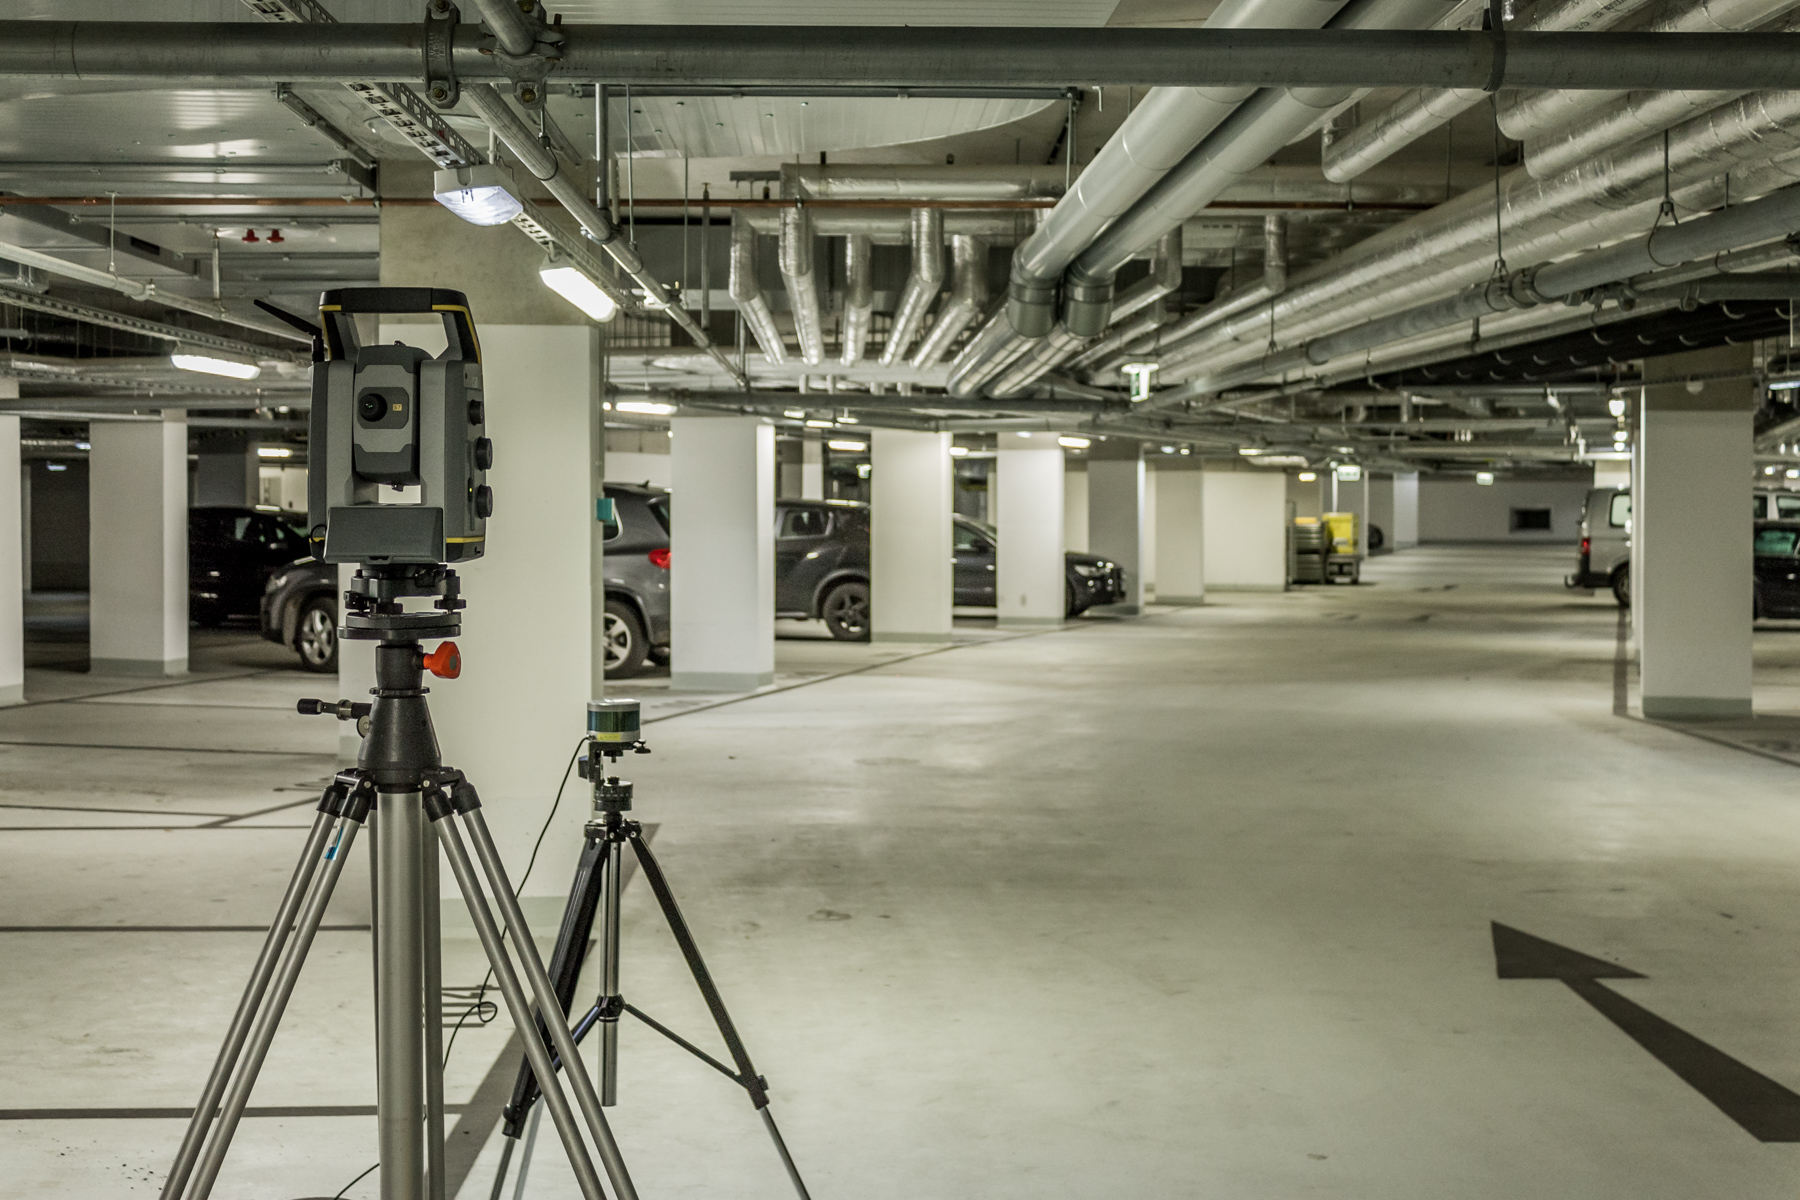
\includegraphics[width=0.45\textwidth]{./img/tiefgarage.jpg}
 % Strahlengang.eps: 0x0 pixel, 300dpi, 0.00x0.00 cm, bb=0 0 3066 4000
 \caption{Vergleichsmessungen mit dem Velodyne VLP-16, Zoller+Fröhlich Imager 5010 und dem Trimble S7}
 \label{img:messbilder}
\end{figure}

\paragraph{Fehler im Skript} Bei der Auswertung der Messung der Tiefgarage (\autoref{img:messbilder}, rechts) fiel schon vor dem Vergleich mit der Tachymetermessung auf, dass die Messwerte sich von Drehung zu Drehung des VLP-16 in Rotationsrichtung verschoben waren. Die Analyse ergab einen Umformungsfehler in der Klasse \code{VdDataset}. Hierdurch wurden die Horizontalrichtungen um bis zu 2 Grad (bei 1200 Umdrehungen pro Minute) fehlerhaft berechnet (siehe \autoref{img:fehlerWolke}). Bei der Messung der Tiefgarage wurden glücklicherweise auch die Rohdaten von 2 von 5 Messreihen gespeichert, so dass hier keine erneute Messung vor Ort nötig war. Die Daten der Fassadenmessung (\autoref{img:messbilder}, links) mussten nochmals wiederholt werden, da die Daten auch durch speziell entwickelte Skripts nicht auswertbar zu korrigieren waren.

\begin{figure}
 \centering
 
\includegraphics[width=0.45\textwidth]{./img/punktwolke_f.png}
 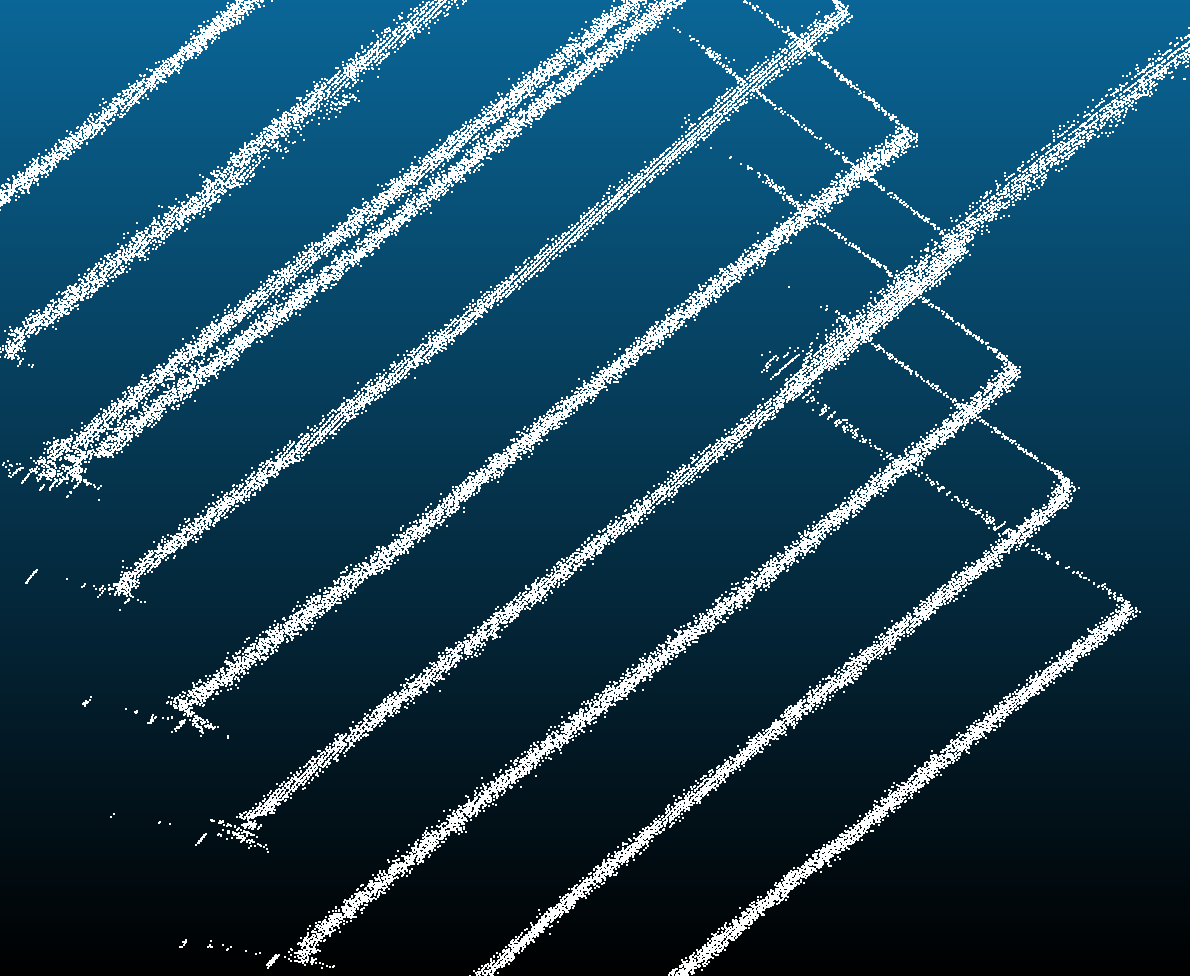
\includegraphics[width=0.45\textwidth]{./img/punktwolke_k.png}
 % Strahlengang.eps: 0x0 pixel, 300dpi, 0.00x0.00 cm, bb=0 0 3066 4000
 \caption{Punktwolke des Velodyne VLP-16 vor (links) und nach (rechts) der Korrektur der Horizontalrichtung am Beispiel eines Pfeilers in der Tiefgarage}
 \label{img:fehlerWolke}
\end{figure}

\subsection{Vergleichsmessung an einer Fassadenfront / im geodätischen Labor}
Die erste Messung zur Überprüfung der Entfernungsmessung fand vor einer weißen Fassade der HafenCity Universität statt. Durch einen Fehler im Auswerteskript, der erst bei großen Strecken auffiel, waren die Messdaten jedoch leider nicht zu verwenden. Es wurde daher eine ähnliche Messung im geodätischen Labor nachgeholt (siehe \autoref{img:geoLabor}).
Hier wurde der Velodyne VLP-16 mittig im Raum aufgestellt. Zwei Stellwände wurden zur Überprüfung der Entfernungsmessung verwendet. Eine blieb hierbei immer an der gleichen Stelle, etwa \todo{Entferung} Meter vom Velodyne entfernt stehen, die zweite wurde in verschiedenen Entfernung aufgestellt (zwischen \todo{Entfernung} Meter). Die Messszenarios wurden jeweils mit dem Imager 5010 von Zoller+Fröhlich dokumentiert. Bei Messungen auf weiße Oberflächen liegt die Streckenmessgenauigkeit des Imager 5010 unter einem Millimeter \citep{imager5010}. Zum Vergleich mit dem Velodyne VLP-16, der eine angegebene Genauigkeit von 3 Zentimetern hat \citep{vlpSheet}, wird die Messung des Imagers daher als wahrer Wert angenommen.

\begin{figure}
 \centering
 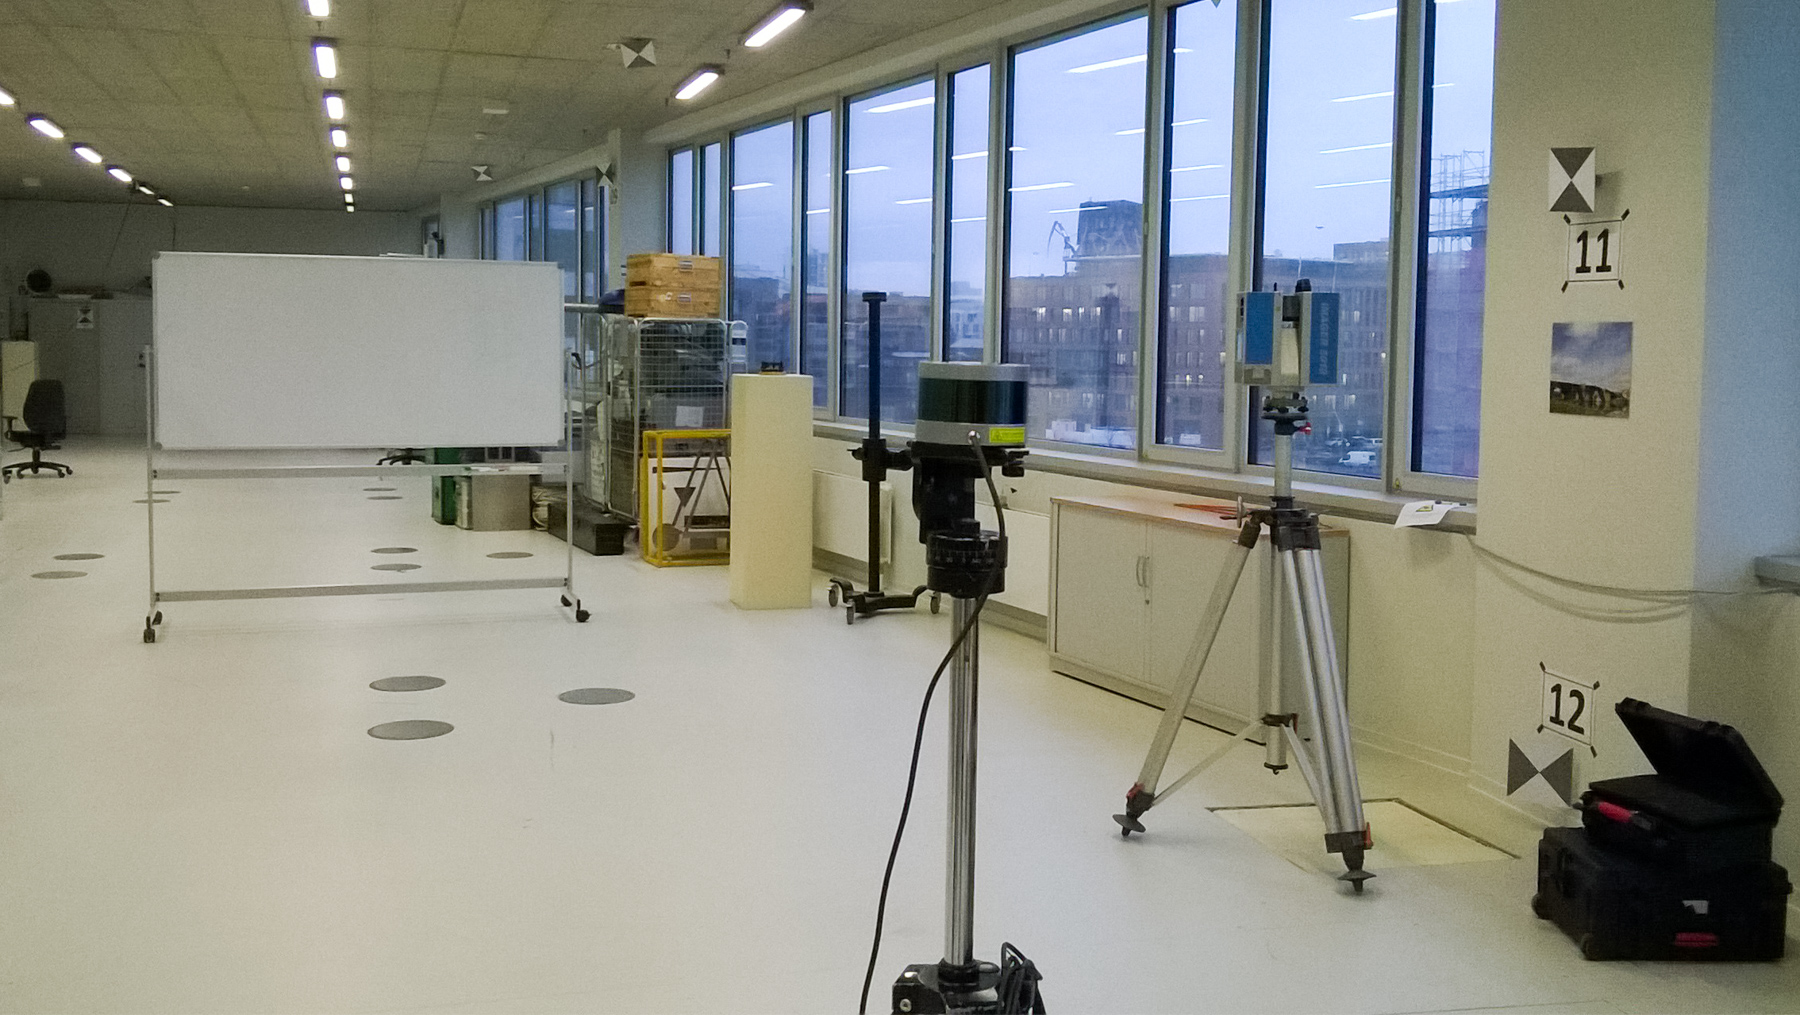
\includegraphics[width=0.7\textwidth]{./img/geoLabor.jpg}
 % Strahlengang.eps: 0x0 pixel, 300dpi, 0.00x0.00 cm, bb=0 0 3066 4000
 \caption{Messung im geodätischen Labor}
 \label{img:geoLabor}
\end{figure}

\paragraph{Nachbearbeitung der Messdaten}
Die Punktwolken des Imager 5010 wurden in der Software Z+F LaserControl des Herstellers über angebrachten Targets zusammengeführt. Anschließend wurden die Punktwolken gefiltert und in die Software Geomagic Wrap importiert. Hier wurde der Standpunkt des Velodyne VLP-16 bestimmt, in dem ein Zylinder gemäß der Größe aus dem Datenblatt \citep{vlpSheet} in die dem VLP-16 zuzuordnenden Punkte der Punktwolke automatisch eingepasst wurde.  Hieraus konnte dann durch Bestimmung der Mittelachse und der Daten des Fokuspunktes der Nullpunkt der Punktwolken des VLP-16 bestimmt werden.
In den Laserpunktwolken der beiden Scanner wurden in Geomagic Wrap die Wände, Decke, Fußboden und die Stellwände modelliert. Hierfür wurden die entsprechenden Punkte ausgewählt und mittels Best-Fit-Anpassung Ebenen in den Punkten ausgeglichen. Über die Wände und Decken wurden die Punktwolken nochmals genauer zu einander ausgerichtet.

\paragraph{Präzision der Streckenmessung}
Beim Modellieren der Wände bestand die Möglichkeit, sich die Genauigkeit der Ausgleichung in den Punkten anzuzeigen. Wie vom Hersteller des Velodyne angegeben, betrug die Standardabweichung dieser Punkte zur durch Ausgleichung bestimmten Ebene bei maximal 3 Zentimetern.

\paragraph{Richtigkeit der Streckenmessung}
Um zu Überprüfen, ob nicht nur die Wiederholungsgenauigkeit des Velodyne VLP-16 im angegeben Bereich liegt, wurden die Positionen der modellierten Stellwände aus den Datensätzen des Velodyne mit denen des Imager 5010 verglichen. Hierzu wurden die Abstände zwischen den Flächen aus beiden Messverfahren jeweils einer Stellwand in CAD bestimmt.
\todo{weiter...}


\subsection{Vergleichsmessung in der Tiefgarage}
Hauptsächlich zur Überprüfung der Genauigkeit der Winkelmessung, aber auch zur Überprüfung der Streckenmessung auf maximaler Entfernung wurde eine weitere Messung in der Tiefgarage durchgeführt. Durch die vielen klaren, rechtwinkligen Kanten, sind hier viele Möglichkeiten um Kanten zu detektieren gegeben. Zum Vergleich wurde die Tiefgarage mit einem Trimble S7 mit einer Winkelgenauigkeit von \todo{Genauigkeit} und einer prismenlosen Streckengenauigkeit von 2 mm + 2 ppm verwendet \citep{trimbles7}.

\paragraph{Auswertung}
Aus den Daten der Tachymetermessung wurden die Wände und Pfeiler der Tiefgarage modelliert. Durch Anpassung der Laserscandaten an diesen Grundriss wurde die Orientierung des Velodyne VLP-16 bestimmt. Die Neigung wurde wiederum durch Ausgleichung der Fußbodenebene durchgeführt. Auch aus den Laserpunktwolken des Velodyne Vlp-16 wurden die Ecken modelliert. Hierfür würden jeweils Ebenen in die Punkte der Pfeiler- und Wandoberflächen in Geomagic Wrap mittels Ausgleichung eingepasst.

\todo{weiter...}

\chapter{Ausblick}
\label{c:ausblick}

\paragraph{Weiterverarbeitung der Daten}
Die Umformung und Speicherung der Daten war nur ein erster Schritt zur Entwicklung des Airborne Laserscanning Systems. Es ist so zwar möglich, die Daten vom Laserscanner, der inertialen Messeinheit und des GNSS zu speichern, jedoch müssen diese Daten weiter prozessiert werden. Bisher wurde der Scanner nur stationär zur Messung eingesetzt. Um  ihn auch kinematisch nutzen zu können, müssen aus den Daten der IMU die Bewegungen rekonstruiert werden. Hiermit können dann die Messungen in ein System überführt werden. Diese Verarbeitung wird in einer Folgearbeit behandelt werden.

\paragraph{Anwendbarkeit des Messsystems}
Da das fertige Messsystem keine Abhängigkeiten vom Multikopter hat, kann es nicht nur fliegend, sondern auch terrestrisch verwendet werden. Einzige Bedingung der Nutzung ist die freie Sicht zum Himmel für den GNSS-Empfang. So wäre auch eine Montage des Systems, gegebenenfalls auch unter Nutzung des Gimbal, an andere, bodengebundene Fahrzeuge denkbar. So ließen sich zum Beispiel zur Digitalisierung von Straßenzügen für 3D-Stadtmodelle zuerst die Straßen und Wege mit Autos, Fahrrädern oder Bollerwagen bodengebunden aufnehmen und mit dem gleichen Messsystem anschließend mit dem Multikopter eine Messung von oben durchführen. So wäre mit einem Messesystem die nahtlose Erfassung von Gebäudehüllen möglich.

\paragraph{Erweiterungs- und Optimierungsmöglichkeiten}
In der Programmierung des Raspberry Pi sind natürlich noch Verbesserungen und Optimierungen möglich. Eine sinnvolle Erweiterung ist zum Beispiel in der Konfigration des Raspberry Pis die Einrichtung als Proxyserver für den Laserscanner, um auch hier Einstellungen mobil durchführen zu können. Programmiertechnisch könnten die restlichen Skripte noch in ihrer Geschwindigkeit der Ausführung optimiert werden.

\todo{Erweitern}



%% Literatur
\renewcommand\UrlFont\itshape
\bibliography{Thesis}

\listoffigures
\listoftables
%\lstlistoflistings

\renewcommand{\appendixpagename}{\appendixname} 
\renewcommand{\appendixtocname}{\appendixname} 
\begin{appendices}

\chapter{Python-Skripte}
\label{a:skripte}
\section{vdAutoStart.py}
\label{a:vdAutoStart.py}
\lstinputlisting[language=Python]{../Quelltext/Python/vdAutoStart.py}

\section{vdBuffer.py}
\label{a:vdBuffer.py}
\lstinputlisting[language=Python]{../Quelltext/Python/vdBuffer.py}

\section{vdTransformer.py}
\label{a:vdTransformer.py}
\lstinputlisting[language=Python]{../Quelltext/Python/vdTransformer.py}

\section{vdInterface.py}
\label{a:vdInterface.py}
\lstinputlisting[language=Python]{../Quelltext/Python/vdInterface.py}

\section{vdGNSSTime.py}
\label{a:vdGNSSTime.py}
\lstinputlisting[language=Python]{../Quelltext/Python/vdGNSSTime.py}

\section{vdHardware.py}
\label{a:vdHardware.py}
\lstinputlisting[language=Python]{../Quelltext/Python/vdHardware.py}

\section{vdFile.py}
\label{a:vdFile.py}
\lstinputlisting[language=Python]{../Quelltext/Python/vdFile.py}

\section{vdASCIIFile.py}
\label{a:vdASCIIFile.py}
\lstinputlisting[language=Python]{../Quelltext/Python/vdASCIIFile.py}

\section{vdTxtFile.py}
\label{a:vdTxtFile.py}
\lstinputlisting[language=Python]{../Quelltext/Python/vdTxtFile.py}

\section{vdObjFile.py}
\label{a:vdObjFile.py}
\lstinputlisting[language=Python]{../Quelltext/Python/vdObjFile.py}

\section{vdXYZFile.py}
\label{a:vdXYZFile.py}
\lstinputlisting[language=Python]{../Quelltext/Python/vdXYZFile.py}

\section{vdSQLite.py}
\label{a:vdSQLite.py}
\lstinputlisting[language=Python]{../Quelltext/Python/vdSQLite.py}

\section{vdDataset.py}
\label{a:vdDataset.py}
\lstinputlisting[language=Python]{../Quelltext/Python/vdDataset.py}

\section{vdPoint.py}
\label{a:vdPoint.py}
\lstinputlisting[language=Python]{../Quelltext/Python/vdPoint.py}

\section{config.ini}
\label{a:config.ini}
\lstinputlisting[]{../Quelltext/Python/config.ini}

\section{convTxt2Obj.py}
\label{a:convToObj.py}
\lstinputlisting[language=Python]{../Quelltext/Python/convTxt2Obj.py}

\section{convBin2Obj.py}
\label{a:convBin2Obj.py}
\lstinputlisting[language=Python]{../Quelltext/Python/convBin2Obj.py}

\chapter{C++-Quelltexte}
\label{a:cpp}

\section{main.cpp}
\label{a:main.cpp}
\lstinputlisting[language=C++]{../Quelltext/C++/src/main.cpp}

\section{VdFile.h}
\label{a:VdFile.h}
\lstinputlisting[language=C++]{../Quelltext/C++/src/VdFile.h}

\section{VdFile.cpp}
\label{a:VdFile.cpp}
\lstinputlisting[language=C++]{../Quelltext/C++/src/VdFile.cpp}

\section{VdASCIIFile.h}
\label{a:VdASCIIFile.h}
\lstinputlisting[language=C++]{../Quelltext/C++/src/VdASCIIFile.h}

\section{VdASCIIFile.cpp}
\label{a:VdASCIIFile.cpp}
\lstinputlisting[language=C++]{../Quelltext/C++/src/VdASCIIFile.cpp}

\section{VdObjFile.h}
\label{a:VdObjFile.h}
\lstinputlisting[language=C++]{../Quelltext/C++/src/VdObjFile.h}

\section{VdObjFile.cpp}
\label{a:VdObjFile.cpp}
\lstinputlisting[language=C++]{../Quelltext/C++/src/VdObjFile.cpp}

\section{VdTxtFile.h}
\label{a:VdTxtFile.h}
\lstinputlisting[language=C++]{../Quelltext/C++/src/VdTxtFile.h}

\section{VdTxtFile.cpp}
\label{a:VdTxtFile.cpp}
\lstinputlisting[language=C++]{../Quelltext/C++/src/VdTxtFile.cpp}

\section{VdXYZFile.h}
\label{a:VdXYZFile.h}
\lstinputlisting[language=C++]{../Quelltext/C++/src/VdXYZFile.h}

\section{VdXYZFile.cpp}
\label{a:VdXYZFile.cpp}
\lstinputlisting[language=C++]{../Quelltext/C++/src/VdXYZFile.cpp}

\section{VdSQLite.h}
\label{a:VdSQLite.h}
\lstinputlisting[language=C++]{../Quelltext/C++/src/VdSQLite.h}

\section{VdSQLite.cpp}
\label{a:VdSQLite.cpp}
\lstinputlisting[language=C++]{../Quelltext/C++/src/VdSQLite.cpp}

\section{VdDataset.h}
\label{a:VdDataset.h}
\lstinputlisting[language=C++]{../Quelltext/C++/src/VdDataset.h}

\section{VdDataset.cpp}
\label{a:VdDataset.cpp}
\lstinputlisting[language=C++]{../Quelltext/C++/src/VdDataset.cpp}

\section{VdPoint.h}
\label{a:VdPoint.h}
\lstinputlisting[language=C++]{../Quelltext/C++/src/VdPoint.h}

\section{VdPoint.cpp}
\label{a:VdPoint.cpp}
\lstinputlisting[language=C++]{../Quelltext/C++/src/VdPoint.cpp}

\section{VdXYZ.h}
\label{a:VdXYZ.h}
\lstinputlisting[language=C++]{../Quelltext/C++/src/VdXYZ.h}

\section{VdXYZ.cpp}
\label{a:VdXYZ.cpp}
\lstinputlisting[language=C++]{../Quelltext/C++/src/VdXYZ.cpp}

\chapter{Beispieldateien}

\section{Rohdaten vom Scanner}
\label{a:Rohdaten}

{\color{gray} Netzwerk-Header}\\
{\color{red} Flag (FF EE)} {\color{green} Horizontalrichtung}\\
{\color{blue} Strecke} {\color{orange} Reflektivität}\\
{\color{yellow} Timestamp } {\color{violet} Return-Modus}\\
\\

\newcommand\tab[1][1cm]{\hspace*{#1}}
\noindent\code{0000\tab{\color{gray} ff ff ff ff ff ff 60 76 88 00 00 00 08 00 45 00}\\
0010\tab{\color{gray} 04 d2 00 00 40 00 ff 11 b4 aa c0 a8 01 c8 ff ff}\\
0020\tab
{\color{gray} ff ff 09 40 09 40 04 be 00 00}
{\color{red} ff ee} {\color{green} 02 4d}
{\color{blue} 00 00}\\
0030\tab
{\color{orange} 0f}
{\color{blue} 00 00} {\color{orange} 0a}
{\color{blue} 00 00} {\color{orange} 16}
{\color{blue} f0 01} {\color{orange} 04}
{\color{blue} 00 00} {\color{orange} 0d}
{\color{blue} 00 00} {\color{orange} 0a}\\
0040\tab
{\color{blue} 00 00} {\color{orange} 0d}
{\color{blue} 00 00} {\color{orange} 06}
{\color{blue} 00 00} {\color{orange} 0b}
{\color{blue} 00 00} {\color{orange} 08}
{\color{blue} 00 00} {\color{orange} 10}
{\color{blue} 00}\\
0050\tab
{\color{blue} 00} {\color{orange} 05}
{\color{blue} 92 01} {\color{orange} 05}
{\color{blue} 00 00} {\color{orange} 04}
{\color{blue} 00 00} {\color{orange} 0f}
{\color{blue} 00 00} {\color{orange} 07}
{\color{blue} 00 00}\\
0060\tab
{\color{orange} 0f}
{\color{blue} 00 00} {\color{orange} 0a}
{\color{blue} 00 00} {\color{orange} 16}
{\color{blue} e6 01} {\color{orange} 08}
{\color{blue} 00 00} {\color{orange} 0d}
{\color{blue} 00 00} {\color{orange} 0a}\\
0070\tab
{\color{blue} 00 00} {\color{orange} 0d}
{\color{blue} 00 00} {\color{orange} 06}
{\color{blue} 00 00} {\color{orange} 0b}
{\color{blue} 00 00} {\color{orange} 08}
{\color{blue} 00 00} {\color{orange} 10}
{\color{blue} 00}\\
0080\tab
{\color{orange} 00 05}
{\color{blue} 7e 01} {\color{orange} 05}
{\color{blue} 00 00} {\color{orange} 04}
{\color{blue} 00 00} {\color{orange} 0f}
{\color{blue} 00 00} {\color{orange} 07}
{\color{red} ff ee}\\
0090\tab
{\color{green} 02 4d}
{\color{blue} 00 00} {\color{orange} 0f}
{\color{blue} 00 00} {\color{orange} 0a}
{\color{blue} 00 00} {\color{orange} 16}
{\color{blue} f0 01} {\color{orange} 04}
{\color{blue} 00 00}\\
...\\
04d0\tab
{\color{orange} 05}
{\color{blue} 00 00} {\color{orange} 04} 
{\color{blue} 00 00} {\color{orange} 0f}
{\color{blue} 00 00} {\color{orange} 07}
{\color{yellow} 8c 25 44 63} {\color{violet} 39 22}
}


\section{Dateiformat für Datenspeicherung als Text}
\label{a:AusgabeTXT}
\lstinputlisting[firstline=1, lastline=20]{../Aufzeichnungen/test.txt}

\section{Dateiformat für Datenspeicherung als OBJ}
\label{a:AusgabeOBJ}
\lstinputlisting[firstline=1, lastline=20]{../Aufzeichnungen/test.txt.obj}


\end{appendices}

\newpage
\noindent\textbf{\large Erklärung}\\
Hiermit versichere ich, dass ich die beiliegende Bachelor-Thesis ohne fremde Hilfe selbst\-stän\-dig verfasst und nur die angegebenen Quellen und Hilfsmittel benutzt habe.\\
\\
Wörtlich oder dem Sinn nach aus anderen Werken entnommene Stellen sind unter Angabe der Quellen kenntlich gemacht. 
\\
\\
\\
\\
\noindent{\underline{Hamburg, den 12. Dez. 2017~\hspace{10cm}}}\\
\noindent{\small Ort, Datum \hspace{4.5cm} Florian Timm}


\end{document}